\documentclass[11pt]{article}
\usepackage{amsfonts}
\usepackage{hyperref}
\usepackage{graphicx,subfigure}
\usepackage{epsfig}
\usepackage{hyperref}
\usepackage{amsmath}
\usepackage{amssymb}
\usepackage{algorithm}
\usepackage{algorithmic}
\usepackage{url}
\usepackage{enumerate}
\usepackage{amsfonts}
\usepackage{boxedminipage}
\usepackage{xcolor}
 \usepackage{framed}
\usepackage{rotating}
\usepackage{soul}
\usepackage{mathtools}
\usepackage{cancel}
%\usepackage{palatino}
\usepackage{setspace}

\usepackage{array}
\usepackage{multirow}
\usepackage{color}
\usepackage{tikz}


\usepackage{mathabx}
\usepackage{tabularx,ragged2e,booktabs,caption}
\usepackage{enumitem}
\newcommand{\overbar}[1]{\mkern 1.5mu\overline{\mkern-1.5mu#1\mkern-1.5mu}\mkern 1.5mu}

\oddsidemargin=0.15in
\evensidemargin=0.15in
\topmargin=-.5in
\textheight=9in
\textwidth=6.25in

\DeclarePairedDelimiter{\floor}{\lfloor}{\rfloor}
\DeclarePairedDelimiter{\ceil}{\lceil}{\rceil}
\DeclareGraphicsExtensions{.gif, .ps, .eps, .png}
\DeclareGraphicsRule{.gif}{png}{}{`convert #1 'png:-'}

\DeclareGraphicsExtensions{.gif, .ps, .eps, .png}
\DeclareGraphicsRule{.gif}{png}{}{`convert #1 'png:-'}

\newcommand{\inprod}[2]{\left\langle #1,#2\right\rangle}
\newcommand{\norm}[1]{\left\| #1\right\|}
\newcommand{\pmat}[1]{\begin{pmatrix} #1\end{pmatrix}}
\newcommand{\cB}{\mathcal{B}}
\newcommand{\bN}{\mathbb{N}\,}

\newcommand*{\vertbar}{\rule[-1ex]{0.5pt}{2.5ex}}
\newcommand*{\horzbar}{\rule[.5ex]{2.5ex}{0.5pt}}

\newcommand{\R}{\ensuremath{\mathbb{R}}}
 % \newcommand{\E}{\ensuremath{\mathbb{E}}}
  \newcommand{\N}{\ensuremath{\mathbb{N}}}
  %newcommand{\C}{\ensuremath{\mathbb{C}}}
  \newcommand{\Tr}{\ensuremath{\top}}
  \newcommand{\Prob}{\ensuremath{\mathbb{P}}}
  \newcommand{\Nc}{\mathcal{N}}
\newcommand{\innerr}[2]{{\left\langle #1\,,\,#2 \right\rangle}}

  % IML
  % ----
  \newcommand{\Xc}{\mathcal{X}}
  \newcommand{\Yc}{\mathcal{Y}}
  \newcommand{\Hc}{\mathcal{H}}
  \newcommand{\Ac}{\mathcal{A}}
  \newcommand{\Dc}{\mathcal{D}}
  \newcommand{\Fc}{\mathcal{F}}
  \newcommand{\Rc}{\mathcal{R}}
%\newcommand{\inner}[2]{{\left\langle #1\,,\,#2 \right\rangle}}

   \newcommand{\blue}{\color{blue}}
   \newcommand{\red}{\color{red}}
\newcommand{\cov}{\mathrm{Cov}}

\newenvironment{myalgo}[1]%
{
%\vspace{0.3cm}
\begin{center}
\begin{boxedminipage}{0.8\linewidth}
\begin{center}
\textbf{\texttt{#1}}
\end{center}
\rm
\begin{tabbing}
....\=...\=...\=...\=...\=  \+ \kill
} %
{\end{tabbing} 
\end{boxedminipage} \end{center} %\vspace{0.3cm}
}


  % ---

%\newcommand{\norm}[1]{\left|\left| #1 \right|\right|}


\newcommand{\plim}{\stackrel{p}{\rightarrow}}
\newcommand{\aslim}{\stackrel{a.s.}{\rightarrow}}
\newcommand{\dlim}{\stackrel{d}{\rightarrow}}

% distributed as
\newcommand{\iid}{\stackrel{\text{iid}}{\sim}}
\newcommand{\ind}{\stackrel{\text{ind.}}{\sim}}
\newcommand{\indep}{\stackrel{\text{indep.}}{\sim}}
\newcommand{\VV}[1]{\mathbf{#1}}
\newcommand{\Vhat}[1]{\ensuremath{\hat{\mathbf{#1}}}}

\newcommand{\GILAD}[1]{ 
    {\color{cyan}  Gilad: #1}
}
\newcommand{\URY}[1]{
    {\color{orange} Ury: #1}
}
\newcommand{\MATAN}[1]{ 
    {\color{red}  Matan: #1}
}
\newcommand{\OTHER}[1]{ 
    {\color{blue}  Other: #1}
}


\title{Statistical Learning for Computer Science Students}

\date{March 2020}



\usepackage{graphicx,subfigure}
% As of 2010, we use the hyperref package to produce hyperlinks in the
% resulting PDF.  If this breaks your system, please commend out the
% following usepackage line and replace \usepackage{icml2011} with
% \usepackage[nohyperref]{icml2011} above.
\usepackage{hyperref}

% \usepackage{icml2011}

\usepackage{amsmath}
\usepackage{amssymb}

\usepackage{algorithm}
\usepackage{algorithmic}
\algsetup{indent=2em}


%% \usepackage{rotating}
%% \usepackage{array}
%% \usepackage{multirow}
%% \usepackage{color}

%% \usepackage{tikz}

\usepackage{url}

\newtheorem{definition}{Definition}
\newtheorem{lemma}{Lemma}
\newtheorem{corollary}{Corollary}
\newtheorem{theorem}{Theorem}
\newtheorem{proposition}{Proposition}
\newtheorem{assumption}{Assumption}
\newtheorem{example}{Example}
\newtheorem{remark}{Remark}
\newtheorem{claim}{Claim}
\newtheorem{exercise}{Exercise}
\newtheorem{discussion}{Discussion}


\newcommand{\gb}[1]{{\boldsymbol{#1}}}
\newcommand{\valpha}{\gb{\alpha}}
\newcommand{\vmu}{\gb{\mu}}
\newcommand{\vnu}{\gb{\nu}}
\newcommand{\vxi}{\gb{\xi}}
\newcommand{\vtheta}{\gb{\theta}}
\newcommand{\vrho}{\gb{\rho}}
\newcommand{\vbeta}{\gb{\beta}}
\newcommand{\vtau}{\gb{\tau}}
\newcommand{\vbalpha}{\gb{\alpha^\star}}
\newcommand{\vbbeta}{\gb{\beta^\star}}
\newcommand{\vtalpha}{\gb{\tilde{\alpha}}}
\newcommand{\vlambda}{\gb{\lambda}}
\newcommand{\slambda}{\bar{\vlambda}}
\newcommand{\stheta}{\bar{\vtheta}}
\newcommand{\vphi}{\gb{\phi}}
\newcommand{\vsigma}{\gb{\sigma}}

\newcommand{\x}{{\mathbf x}}
\newcommand{\y}{{\mathbf y}}
\newcommand{\z}{{\mathbf z}}
\newcommand{\w}{{\mathbf w}}
\newcommand{\bw}{\bar{\w}}
\newcommand{\bF}{\bar{F}}
\renewcommand{\v}{{\mathbf v}}
\renewcommand{\u}{{\mathbf u}}
\newcommand{\e}{{\mathbf e}}
\newcommand{\bsig}{{\mathbf \sigma}}
\newcommand{\rE}{{\mathbf E}}
\newcommand{\sgn}{{\mathrm{sgn}}}
\newcommand{\cF}{{\cal F}}
\newcommand{\pr}{\mathbb{P}}
\newcommand{\rV}{{\mathrm {Var}}}
\newcommand{\tr}{{\mathrm{tr}}}
\newcommand{\trans}{\dagger}
\newcommand{\diag}{{\mathrm{diag}}}
\newcommand{\lspan}{{\mathrm{span}}}
\renewcommand{\r}{{\mathbf{r}}}
\newcommand{\tL}{\tilde{L}}
\newcommand{\hL}{\hat{L}}

\newcommand{\cD}{\mathcal{D}}
\newcommand{\bE}{\mathbb{E}\,}


\newcommand{\BlackBox}{\rule{1.5ex}{1.5ex}}
\newenvironment{proof}{\par\noindent{\bf Proof\ }}{\hfill\BlackBox\\[2mm]}

\newcommand{\reals}{\mathbb{R}}
\newcommand{\Y}{\mathcal{Y}}
\newcommand{\X}{\mathcal{X}}
\renewcommand{\H}{\mathcal{H}}
\newcommand{\E}{\mathbb{E}}
\newcommand{\D}{\mathcal{D}}
\newcommand{\V}{\mathcal{V}}
%\newcommand{\U}{\mathcal{U}}
\newcommand{\F}{\mathcal{F}}
\newcommand{\inner}[1]{\langle #1 \rangle}
\newcommand{\half}{\frac{1}{2}}
\newcommand{\thalf}{\tfrac{1}{2}}
\newcommand{\eqdef}{\stackrel{\mathrm{def}}{=}}
\newcommand{\err}{\mathrm{err}}
\newcommand{\opt}{\mathrm{opt}}
\newcommand{\herr}{\widehat{\err}}
\newcommand{\hopt}{\hat{\opt}}
\newcommand{\eopt}{\epsilon_{\mathrm{opt}}}
\newcommand{\eapp}{\epsilon_{\mathrm{app}}}
\newcommand{\eest}{\epsilon_{\mathrm{est}}}
\newcommand{\halg}{\tilde{h}}
\newcommand{\empf}{\hat{F}_{\lambda}}
\newcommand{\T}{\mathrm{time}}
\newcommand{\erf}{\mathrm{erf}}
\newcommand{\sig}{\mathrm{sig}}
\newcommand{\poly}{\mathrm{poly}}

\newcommand{\rank}{\mathrm{rank}}
\newcommand{\supp}{\mathrm{supp}}
\newcommand{\spn}{\mathrm{span}}
\newcommand{\image}{\mathrm{image}}


\DeclareMathOperator*{\argmin}{argmin} % Declares argmin and ensures super and subscripts are located nicely above/below such as in \min
\DeclareMathOperator*{\argmax}{argmax} % Declares argmin and ensures super and subscripts are located nicely above/below such as in \min
\DeclareMathOperator*{\prob}{\mathbb{P}}

\renewcommand{\eqref}[1]{Equation~(\ref{#1})}
\newcommand{\figref}[1]{Figure~\ref{#1}}
\newcommand{\secref}[1]{Section~\ref{#1}}
\newcommand{\thmref}[1]{Theorem~\ref{#1}}
\newcommand{\lemref}[1]{Lemma~\ref{#1}}
\newcommand{\defref}[1]{Definition~\ref{#1}}
\newcommand{\corref}[1]{Corollary~\ref{#1}}

%\newcommand{\comment}[1]{\textcolor{red}{\textbf{#1}}}
\newcommand{\mathcomment}[1]{\color{red}{\textbf{#1}}}

\newcommand{\indct}[1]{\boldsymbol{1}\!\left[ #1 \right]}

\newcommand{\blambda}{\bar{\lambda}}
\newcommand{\bA}{\bar{A}}
\newcommand{\bI}{\bar{I}}

\newcommand{\vect}{\mathrm{vec}}


\newcommand{\coursename}{Introduction to Machine Learning (67577)}

\newcommand{\handout}[5]{
%   \renewcommand{\thepage}{#1-\arabic{page}}
   \noindent
   \begin{center}
   \framebox{
      \vbox{
    \hbox to 5.78in { {\bf \coursename}
         \hfill #2 }
       \vspace{4mm}
       \hbox to 5.78in { {\Large \hfill #5  \hfill} }
       \vspace{2mm}
       \hbox to 5.78in { {\it #3 \hfill #4} }
      }
   }
   \end{center}
   \vspace*{4mm}
}

\newcommand{\notes}[5]{
%   \renewcommand{\thepage}{#1-\arabic{page}}
   \noindent
   \begin{center}
    \hbox to 5.78in { {\bf \coursename}  \hfill #2}
       \vspace{14mm}
       \hbox to 5.78in { {\Large \hfill #5  \hfill} }
   \end{center}
   \vspace*{4mm}
}

% Lecture notes:
\newcommand{\lecture}[5]{\handout{#1}{#3}{Lecturer:
#4}{Scribe: #5}{Lecture #1: #2}}

\newcommand{\recitation}[5]{\handout{#1}{#3}{#4}{ #5}{Recitation #1: #2}}

% Exam:
\newcommand{\exam}[1]{\handout{#1}{}{}{}{Exam}}
\newcommand{\homeexam}[2]{\handout{#1}{}{}{Due:
#2}{Home Exam}}
\newcommand{\examanswer}[1]{\handout{X}{}{by: #1}{}{Exam - Answers}}

% New exercise
\newcommand{\problemset}[2]{\handout{#1}{}{}{Due:
#2}{Problem Set #1}}

% School solution
\newcommand{\solution}[2]{\handout{#1}{}{}{Written by: #2}{Problem Set #1 - Solution}}

% Submitted solution
\newcommand{\exanswer}[2]{\handout{#1}{}{by: #2}{}{Problem Set #1 - Answers}}

\begin{document}
\maketitle

\tableofcontents

%\onehalfspacing

%\newpage
%\section*{Preface}
%\label{sec:preface}
%\addcontentsline{toc}{sec}{\nameref{sec:preface}}
%This is preface

\newpage
\part*{Introduction}
\label{part:intro}
\addcontentsline{toc}{part}{\nameref{part:intro}}
This is intro
%\input{intro}

\newpage
\part*{Lecture 1: Mathematical Background}
\label{part:lecture_1}
\addcontentsline{toc}{part}{\nameref{part:lecture_1}}
\section{Recap: Probability and Statistics}
\subsection{Probability Space} 
Our intuitive notion of probability is related to uncertainty we have about events in the world, for example - will it rain tomorrow? How much will I get in the final exam? Although we cannot predict with certainty the answers to these questions, we usually know what is the set of all possible outcomes. This gives us the first ingredient in any \emph{probability space}.
\footnote{This section is based on lecture notes by Michal Moshkovitz and Alon Gonen}
\begin{definition}
A \emph{sample space} $\Omega$ is a set that contains all possible outcomes. $\omega\in\Omega$ denotes a single outcome.
\end{definition}
Examples:
\begin{itemize}
\item Coin toss: $\Omega=\left\{ H,T\right\} $
\item Toss a coin until heads comes up: $\Omega=\left\{ T^{n-1}H:n\in\mathbb{N}_0\right\} $
\item Rolling two dice: $\Omega=\left\{ 1,\dots,6\right\} ^{2}$
\item Waiting time at the post office: $\Omega=[0,\infty)$
\end{itemize}
Suppose someone threw a die (singular of dice), and told us that the result is an even number. This result is not an element in $\Omega$, but it tells us that the outcome is an element in the subset $\left\{ 2,4,6\right\} $.
\begin{definition}
An \emph{event} $A$ is any subset of possible outcomes, $A\subseteq\Omega$.
\end{definition}
Quick reminder:
\begin{itemize}
\item $A^{c}$ (or sometimes $\overline{A}$) denotes the \textit{complement} of $A$, $A^{c}=\Omega\backslash A$ . In other words, $A^{c}$ is the event that $A$ did not occur.
\item We say that $A$ and $B$ are \textit{disjoint events} if $A\cap B=\emptyset$.
\item $\Omega$ and $\emptyset$ are also events. If $A$ and $B$ are two events, then $A\cup B$ is also an event, and so is $A\cap B$.
\end{itemize}

Intuitively, a probability function assigns to an event a number which quantifies our knowledge or belief about the possibility of observing any outcome in that event.


%\subsubsection*{Discrete models }
\begin{definition}
A \emph{probability space} is a tuple \footnote{For our needs this simple and intuitive definition is sufficient, though, richer definitions exist.} $(\Omega, \cD)$ where $\Omega$ is a \emph{sample space} and $\cD:2^{\Omega}\rightarrow\reals$ is a probability function such that
\begin{enumerate}
\item $\cD(\Omega)=1$
\item for all $\omega\in\Omega, \cD(\omega)\in[0,1]$
\item for all $A,B\subseteq\Omega$ such that $A\cap B=\emptyset,$ we have $\cD(A \cup B)=\cD(A)+\cD(B).$
\end{enumerate}
\end{definition}
%\begin{exercise} Find he probability space that corresponds to a fair coin toss.
%\end{exercise}
%Solution: $\Omega=\{H,T\},\Pr(H)=\Pr(T)=0.5$
\begin{example}
Suppose we throw two fair dice, then $\Omega=\left\{ 1,\dots,6\right\} ^{2}$ and $\cD\left(\left(i,j\right)\right)=\frac{1}{36}$
\end{example}

\begin{exercise}
For all $A,B\subseteq\Omega$: $\cD(A\cup B)=\cD(A)+\cD(B)-\cD(A\cap B)$
\end{exercise}
Solution:\\
$A\cup B=(A\setminus B)\cup(B\setminus A)\cup(A\cap B)\; ,A=(A\setminus B)\cup(A\cap B)$ and $B=(B\setminus A)\cup(A\cap B).$
$$\cD(A\cup B)=\cD(A\setminus B)+\cD(B\setminus A)+\cD(A\cap B)=\cD(A)-\cD(A\cap B)+\cD(B) - \cancel{\cD(A\cap B)}  + \cancel{\cD(A\cap B)} $$

\begin{definition}
$A,B\subseteq\Omega$ are called \emph{independent} if the occurrence of one does not affect the probability of occurrence of the other. Consequently: $$\cD(A\cap B) =\cD(A)\cdot\cD(B).$$
\end{definition}

\begin{exercise}
If $A$ and $B$ are independent then $A$ and $B^c$ are also independent.
\end{exercise}
Solution: $\cD(A)=\cD(A\cap B)+\cD(A\cap B^c)\Rightarrow\cD(A\cap B^c)=\cD(A)(1-\cD(B))=\cD(A)\cdot\cD(B^c).$\\


\begin{lemma}  \label{lem:unionBound}  \textbf{(The union bound)} Let
$(\Omega, \cD)$ be a probability space. The probability function is \emph{sub-additive}, i.e., for any sequence $(A_k)$ of events,
\[
\cD(\cup_{k=1}^\infty A_k) \le \sum_{k=1} ^\infty \cD(A_k)
\]
\end{lemma}
\begin{proof}
Let $B_1=A_1$. For each $k \in \{2,3,\ldots\}$, let $B_k = A_k
\setminus \cup_{i=1}^{k-1} A_i$. Note that the $B_1...B_k$ are disjoint, and
$\cup_{i=1}^k A_i=\cup_{i=1}^k B_i$. Also, since $B_k\subseteq A_k$, $\cD(B_k) \le \cD(A_k)$ for every $k \in \bN$. It follows by the countable additivity of $\cD$ that
\[
\cD(\cup_{k=1}^\infty A_k) = \cD(\cup_{k=1}^\infty B_k) = \sum_{k=1}
^\infty \cD(B_k) \le \sum_{k=1}
^\infty \cD(A_k)~.
\]
\end{proof}




\subsection{Random Variables, discrete and continuous}

So far we have asked questions like: does an event happen or not and what is the probability of the event. But what about different questions- such as  "how much." For example, if we get a dollar if a coin flip turns head, we can ask how many dollars would we get after 3 rounds? \\

In order to answer this question, we should understand the sample space, which is
 $\Omega=\{HHH,HHT,HTH,THH,HTT,THT,TTH,TTT\}$. Then we would need to define a reward function that will quantify ones's profit for each outcome of the experiment ($\omega\in \Omega$):
 $M(HHH)=3,M(HHT)=2.$ This quantifying function $M$ is called a \emph{random variable} (RV).
\begin{definition}
Given a probability space $\left(\Omega,\cD\right)$, a real-valued \emph{random variable (RV)} is a function $X:\Omega\rightarrow\mathbb{R}$.

\end{definition}
\begin{remark}
Any function $g\left(X\right)$ of a random variable is also a random
variable (for instance $X^{2}$, $\sgn \left(X\right)$, etc.).
\end{remark}
For a discrete $\Omega$ we define the \textbf{\textit{probability
mass function (PMF)}} of $X$ (a \textit{discrete RV}) as
\[
\cD\left(\left\{ X=x\right\} \right)=\sum_{\omega:X\left(\omega\right)=x}\cD\left(\omega\right)
\]


Instead of writing $\cD\left(\left\{ X=x\right\} \right)$ we usually
write $\cD\left(x\right)$.

\begin{example}
A fair coin is tossed twice. The probability space is given by $\Omega=\left\{ T,H\right\} ^{2}$
and  $\cD\left(\omega\right)=\frac{1}{4}$ for any $\omega\in \Omega$. Let $X$ denote the number of heads obtained in each outcome ($\omega$). The image of $X$ is  $\mathcal{X}=\left\{ 0,1,2\right\} $
and
\[
\cD\left(x\right)=\begin{cases}
\frac{1}{4} & x=0,2\\
\frac{1}{2} & x=1\\
0 & \mbox{else}
\end{cases}
\]

\end{example}


For a continuous $\Omega$ - we say that $X$ is a \textit{continuous
RV} if there exists $f(x)\ge 0$ so that we can write, for every $D\subset\mathbb{R}$
\[
\cD\left(X\in D\right)=\int_{D}f\left(x\right)dx
\]


In particular, this means that for any $a,b\in \mathbb{R}$, where $a\leq b$:
\[
\cD\left(X\in\left[a,b\right]\right)=\int_{a}^{b}f\left(x\right)dx
\]

In this course we assume that $f(x)$ is a regular function and therefore the probability mass function for a single point is 0: $\cD\left(X=a\right)=\int_{a}^{a}f\left(x\right)dx=0$ for any $a\in\mathbb{R}$.

The function $f$ is called the \textbf{\textit{probability density
function }}\textbf{(PDF)} of $X$. Note that -
\begin{itemize}
\item $f\left(x\right)\ge0$
\item $\int_{-\infty}^{\infty}f\left(x\right)dx=1$
\item $f\left(x\right)$ is a probability \emph{density}, not a probability. For example, it could be that $f\left(x\right)>1$.\\
\end{itemize}

\subsection{Mean and Variance}
\begin{definition}
The \textbf{\textit{expected value}} of a random variable
$X$ is
\[
\bE\left[X\right]=\sum_{x\in\mathcal{X}}x\cD\left(x\right)\qquad\mbox{or}\qquad \bE\left[X\right]=\int_{-\infty}^{\infty}xf\left(x\right)dx
\]

\end{definition}
Properties:
\begin{itemize}
\item $\bE\left[g\left(X\right)\right]=\sum g\left(x\right)\cD\left(x\right)$,
\item $\bE\left[c\right]=c$
\item Linear: $\bE\left[aX+Y\right]=a\bE\left[X\right]+\bE\left[Y\right]$
\item If $X$ and $Y$ are independent then $\bE\left[XY\right]=\bE\left[X\right]\bE\left[Y\right]$
(explanation: $\bE[XY]=\sum\cD(X=x,Y=y)x\cdot y = \sum_{x,y}\cD(x)\cD(y)xy=\bE[X]\bE[Y]$)
\end{itemize}

\begin{definition}
Let $X$ be a RV with $\bE\left[X\right]=\mu$, then the \textbf{\textit{variance}}
of $X$ is
\[
V\left(X\right)=\bE\left[\left(X-\mu\right)^{2}\right]
\]
The \textbf{\textit{standard deviation}} is defined as $\sigma=\sqrt{V\left(X\right)}$.
\end{definition}
Properties of the variance:
\begin{itemize}
\item $V(X)\geq0$ , ~$V(X)=0\,\iff\,X$ is a constant.
\item $V\left(X\right)=\bE\left[X^{2}\right] - (\bE\left[X\right])^{2}$
\item $V(aX+b)=a^{2}V(X)$
\item $V(X+Y)=\bE\left[\left(X+Y-\bE(X)-\bE(Y)\right)^{2}\right]=V(X)+V(Y)+2\overbrace{\bE\left[\left(X-\bE[X]\right)\left(Y-\bE[Y]\right)\right]}^{\cov\left(X,Y\right)}$
\item If $X_{1},\dots,X_{n}$ are independent then $V\left(\sum X_{i}\right)=\sum V\left(X_{i}\right)$\end{itemize}

\begin{definition}
The \textbf{\textit{covariance}} of $X$ and $Y$ is
\end{definition}
\[
\cov(X,Y)=\bE\left[\left(X-\bE[X]\right)\left(Y-\bE[Y]\right)\right]=\bE\left[XY\right]-\bE[X]\bE[Y]
\]

Properties:
\begin{itemize}
\item $\cov(X,Y)=\cov(Y,X)$
\item $\cov(aX+b,cY+d) = a \cdot c \cdot \cov(X,Y)$
\item $\cov(X,X)=V(X)$
\end{itemize}
%We say that $X$ and $Y$ are \textbf{\emph{uncorrelated}}\emph{ }\textit{\emph{if $\cov\left(X,Y\right)=0$.}}
%\begin{remark}
%If $X$ and $Y$ are uncorrelated it does not imply that they are independent.\end{remark}

\begin{exercise}
Let $Z$ be a Bernoulli random variable. Calculate $Var[Z].$
\end{exercise}
Solution: $Var[Z] = \bE[Z^2] - (\bE[Z])^2 = p-p^2=p(1-p).$


\begin{example}
Find the mean and variance of $X\sim U\left(\left[a,b\right]\right),$ where $U[a,b]$ is the uniform distribution on $[a,b].$
\begin{eqnarray*}
\bE\left[X\right] & = & \frac{1}{b-a}\int_{a}^{b}xdx=\frac{1}{2\left(b-a\right)}\left(b^{2}-a^{2}\right)=\frac{b+a}{2}\\
\bE\left[X^{2}\right] & = & \frac{1}{b-a}\int_{a}^{b}x^{2}dx=\frac{1}{3\left(b-a\right)}\left(b^{3}-a^{3}\right)=\frac{b^{2}+ab+a^{2}}{3}\\
V\left(X\right) & = & \frac{b^{2}+ab+a^{2}}{3}-\frac{\left(b+a\right)^{2}}{4}=\frac{\left(b-a\right)^{2}}{12}
\end{eqnarray*}
\end{example}

\subsection{A little Statistics: Mean and variance estimation}

This is a course in {\em Statistical} Machine Learning. So let's start with a little bit of statistics. Some of you may have never seen statistics before. 
When we study {\em Probability} we assume a known distribution and calculate probability of events of interest. When we we study {\em Statistics} we turn the question on its head: using samples from an unknown probability distribution, we try to {\em estimate} or {\em test} properties of of the unknown distribution. 

Take the mean and variance of a probability distribution for example. 
The mean gives us a taste of around which point the data is distributed. The variance on the other hand gives you a taste of the concentration of the "spread" of the distribution around its mean. 
Low variance usually means that the distribution is highly concentrated around the mean, while high variance means that the distribution is less concentrated there.\\
In a probability course, given that we know the distribution, we learned how to calculate its mean and variance. 
Now we would like to ask a different question. We are given {\em samples} that were drawn from an unkown distribution.
Can we {\em estimate}  the distribution's mean and variance using only those samples?\\

Formally, let $X$ be a random variable, let $p_X$ be its (unknown) distribution, and let $X_1,\ldots,X_n\overset{i.i.d}{\sim} p_X$.
Here, i.i.d  denotes \emph{independent and identically distributed} random variables. We are given \emph{data}
samples: $x_1,\ldots,x_n$, where $x_i$ is a {\em number} - the sample obtained by sampling $X_i$.
In statistics, $\bE[X]$ is called the {\em population} mean and  $V(X)$ is called the population variance. 
So, what is a "reasonable" \textbf{estimator} for $\bE[X]$ and $V(X)$ based only on those $n$ samples?\\

Throughout the course we are going to use the following estimators (commonly denoted with the "hat" symbol $\hat{\circ}$):
\begin{itemize}
    \item Sample mean (an estimator for the population mean)
    \begin{eqnarray*}
    \hat{\mu}_X = \frac{1}{n} \sum_{i=1}^n x_i
    \end{eqnarray*}
    \item Sample variance (an estimator for population variance)
    \begin{eqnarray*}
    \hat{\sigma}_X^2 = \frac{1}{n-1} \sum_{i=1}^n (x_i-\hat{\mu}_X)^2
    \end{eqnarray*}
    % It is important to note that if you do know the mean of the data, then the sample variance will look like that:
    % \begin{eqnarray*}
    % \hat{\sigma}_X^2 = \frac{1}{n} \sum_{i=1}^n (x_i-\mu)^2
    % \end{eqnarray*}
\end{itemize}
{Note the $\frac{1}{n-1}$ factor. Why not use $\hat{\Sigma}_X^2 = \frac{1}{n} \sum_{i=1}^n (x_i-\hat{\mu}_X)^2$ as the variance estimator? \emph{Answer}: calculate the expected value of these estimators and you will find (perhaps surprisingly) that $\bE[\hat{\sigma}_X^2]=V(X)$ while $\bE[\hat{\Sigma}_X^2] = \frac{n-1}{n}V(X)$. So, in expectation, $\hat{\sigma}_X^2$ gets the population variance exactly. When an estimator for some parameter of the unknown distribution gets the desired parameter exactly {\em in expectation}, we call that estimator {\em unbiased} for that parameter. 


We invite you to read some additional material about the sample variance and the population variance {\color{blue}\href{https://www.macroption.com/population-sample-variance-standard-deviation/}{\textbf{here}}}  and {\color{blue}\href{https://en.wikipedia.org/wiki/Bias_of_an_estimator}{\textbf{here}}} if you want to understand the reason for the difference in the formula. \\

\section{High dimensional distributions}
Back to probability. Now, instead of random variables that take real (scalar) value,  we will consider a more general case in which they take vector values in $\reals^d$, where $d\in \bN$.

\subsection{Basic definitions}

\begin{definition}[Random vector]
A finite collection of random variables, denoted $X_1, \dots, X_n$ (defined on a common probability space $(\Omega, \cD)$) is a random (column) vector: $\boldsymbol{X} = (X_1, \dots, X_n)^T$

\end{definition}


\begin{definition}[Joint distribution]
Given random variables $X_1, \dots, X_n$ , that are defined on a probability space, the joint probability distribution for $X_1, \dots, X_n$ is a probability distribution that gives the probability that each of $X_1, \dots, X_n$ falls in any particular range (for continuous RVs) or discrete set (for discrete RVs) of values specified for that variable.

\end{definition}


\begin{definition}[Joint PDF of a random vector]
Two random variables $X$ and $Y$ are jointly continuous if there exists a nonnegative function $f_{XY}: \reals^2 \to \reals$, such that, for any set $A \in \reals^2$, we have
$$
\cD\left( (X,Y) \in A \right) = \int_A f_{XY}(x, y) dx dy
$$
The function $f_{XY}(x, y)$ is called the \emph{joint probability density function (JPDF)} of $X$ and $Y$.
This can of course be generalized to any dimension. 

\end{definition}

\begin{remark}[PDF for a random vector]
Given $\boldsymbol{X} = (X_1, \dots, X_n)^T$, each of the scalar random variables $X_1, \dots, X_n$ can be characterized by its PDF. However, unless the scalar RV's are mutually independent, the PDF of each coordinate of a random vector does not completely describe the probabilistic behaviour of the whole vector. For instance, $X_1$ and $X_2$ could have the same PDF, but still the behavior of $\boldsymbol{X} = (X_1, X_2)$ and $\boldsymbol{\Tilde{X}} = (X_1, X_1)$ can be drastically different. For example, consider $X_1 \sim U([-a, a])$ and $X_2 = - X_1$. 

\end{remark}



\subsection{Normal Distribution}
As an example of random vectors, we now consider specific family of distributions- the Multivariate Normal (or Multivariate Gaussian) Distributions. The normal distribution is very useful for many reasons. One reason is the Central Limit Theorem (CLT). You have likely seen the one-dimensional ("univariate") version of the CLT in your probability course. In one of its forms, under some conditions, the CLT states that sample mean of random i.i.d variables (when properly scaled) converges in distribution to the normal distribution. There is a multivariate version of the CLT, which is one reason why you want to be familiar with the multivariate normal distribution. Another reason we like the (multivariate) normal distribution is that many results and methods (such as propagation of uncertainty and least squares parameter fitting) can be derived analytically in explicit form when the relevant variables are (multivariate) normally distributed.

\begin{definition}[Univariate Normal Distribution (namely, in dimension $d=1$)] \label{def: UVN}
A random variable x has a normal distribution with expectation $\mu$ and variance $\sigma^2$ if it has a PDF of the form:
$$f(x) = \frac{1}{\sqrt{2\pi\sigma^2} } e^{ -\frac{(x-\mu)^2}{2\sigma^2} } $$
In this case we write: $x\sim\mathcal{N}({\mu},{\sigma^2})$

\end{definition}
\begin{definition}[Multivariate Normal Distribution] \label{def: MVN}
random vector x has a multivariate normal distribution with expectation $\mu$ and covariance matrix (see definition below) $\Sigma$ if it has a joint PDF of the form:
$$f\left(x\right)=\frac{1}{\sqrt{\left(2\pi\right)^{n}\left|\Sigma\right|}}\exp\left\{ -\frac{\left(x-\mu\right)^{T}\Sigma^{-1}\left(x-\mu\right)}{2}\right\} $$
In this case we write: $x\sim\mathcal{N}(\boldsymbol{\mu},\boldsymbol{\Sigma})$
\end{definition}

\begin{figure}[h!]
  \centering
  \begin{minipage}[b]{0.4\textwidth}
        \includegraphics[scale=0.1]{1D.png}
   \caption{$f(x) = \frac{1}{\sqrt{2\pi\sigma^2} } e^{ -\frac{(x-\mu)^2}{2\sigma^2} } $}
  \end{minipage}
  \hfill
  \begin{minipage}[b]{0.5\textwidth}
       \includegraphics[scale=0.1]{2D.png}
   \caption{
   \begingroup
\footnotesize% \small in 11pt base font is 10pt
2D case of\\ $f\left(x\right)=\frac{1}{\sqrt{\left(2\pi\right)^{2}\left|\Sigma\right|}}\exp\left\{ -\frac{\left(x-\mu\right)^{T}\Sigma^{-1}\left(x-\mu\right)}{2}\right\} $
\endgroup}
  \end{minipage}
\end{figure}

Observe that definition \ref{def: MVN} is generalization of \ref{def: UVN}, i.e. when $d = 1$ both definitions are same.
\\

In some cases we do not care about some of the variables in the distribution. for example, suppose we have joint probability function of the variables "height" and "weight" of some community, but we're only interested in one of them. This lead as to the following definition:

\begin{definition}[Marginal Distribution]
Marginal distribution of a subset of a collection of random variables is the probability distribution of the variables contained in the subset. It gives the probabilities of various values of the variables in the subset without reference to the values of the other variables. It can be written as:
$$p_{X}(x)=\int_{y}p_{X,Y}(x,y)\mathrm{d}y$$
\end{definition}

\begin{exercise}[Marginal of the 1st coord. of a 2D normal RV with diagonal covariance]
Let $x\sim\mathcal{N}(\boldsymbol{\mu},\boldsymbol{\Sigma})$ where $\mu = (\mu_1, \mu_2), \boldsymbol{\Sigma}=\left(\begin{array}{cc}
\sigma_{1}^{2} & 0\\
0 & \sigma_{2}^{2}
\end{array}\right)$.

Find the PDF of the marginal distribution of $x_1$.
\end{exercise}
\noindent
\textbf{Solution:}

Observe that we have:

\begin{align*}
& \frac{1}{\sqrt{\left(2\pi\right)^{n}\left|\Sigma\right|}}\exp\left\{ -\frac{\left(x-\mu\right)^{T}\Sigma^{-1}\left(x-\mu\right)}{2}\right\} \\ &= \frac{1}{\sqrt{\left(2\pi\right)^{2}\left|\left(\begin{array}{cc}
\sigma_{1}^{2} & 0\\
0 & \sigma_{2}^{2}
\end{array}\right)\right|}}\exp\left\{ -\frac{\left(x-\mu\right)^{T}\left(\begin{array}{cc}
\sigma_{1}^{-2} & 0\\
0 & \sigma_{2}^{-2}
\end{array}\right)\left(x-\mu\right)}{2}\right\}\\&
= \frac{1}{\sqrt{\left(2\pi\right)^{2}\sigma_{1}^{2}\sigma_{2}^{2}}}\exp\left\{ -\frac{\left(x-\mu\right)^{T}\left(\begin{array}{cc}
\sigma_{1}^{-2} & 0\\
0 & \sigma_{2}^{-2}
\end{array}\right)\left(x-\mu\right)}{2}\right\} \\&
= \frac{1}{\sqrt{\left(2\pi\right)^{2}\sigma_{1}^{2}\sigma_{2}^{2}}}\exp\left\{ -\frac{1}{2} \left(\frac{x_{1}-\mu_{1}}{\sigma_{1}}\right)^{2} - \frac{1}{2} \left(\frac{x_{2} - \mu_{2}}{\sigma_{2}}\right)^{2}\right\} \\&
=	\frac{1}{\sqrt{\left(2\pi\right)\sigma_{1}^{2}}}\exp\left\{ -\frac{1}{2} \left(\frac{x_{1}-\mu_{1}}{\sigma_{1}}\right)^{2}\right\} \frac{1}{\sqrt{\left(2\pi\right)\sigma_{2}^{2}}}\exp\left\{ -\frac{1}{2} \left(\frac{x_{2}-\mu_{2}}{\sigma_{2}}\right)^{2}\right\}
\end{align*}

Now, since: $\int_{-\infty}^\infty\frac{1}{\sqrt{\left(2\pi\right)\sigma_{2}^{2}}}\exp\left\{ -\frac{1}{2} \left(\frac{x_{2}-\mu_{2}}{\sigma_{2}}\right)^{2}\right\}
\mathrm{d}x_2=1$, we get:

\begin{align*}
&\int_{-\infty}^\infty\frac{1}{\sqrt{\left(2\pi\right)^{n}\left|\Sigma\right|}}\exp\left\{ -\frac{\left(x-\mu\right)^{T}\Sigma^{-1}\left(x-\mu\right)}{2}\right\}\;dx_2 \\ &=\frac{1}{\sqrt{\left(2\pi\right)\sigma_{1}^{2}}}\exp\left\{ -\frac{1}{2} \left(\frac{x_{1}-\mu_{1}}{\sigma_{1}}\right)^{2}\right\}
\int_{-\infty}^\infty\frac{1}{\sqrt{\left(2\pi\right)\sigma_{2}^{2}}}\exp\left\{ -\frac{1}{2} \left(\frac{x_{2}-\mu_{2}}{\sigma_{2}}\right)^{2}\right\}\;dx_2 \\
&=\frac{1}{\sqrt{\left(2\pi\right)\sigma_{1}^{2}}}\exp\left\{ -\frac{1}{2} \left(\frac{x_{1}-\mu_{1}}{\sigma_{1}}\right)^{2}\right\}
\end{align*}

and by definition \ref{def: UVN} we get:
$x_1\sim\mathcal{N}({\mu_1},{\sigma_1^2})$
\\


\subsection{Covariance Matrix}

\begin{definition}[Covariance Matrix]
Recall the population variance $V[X]$ of a scalar (univariate) random variable $X$. What is the proper generalization for the case of a random vector?
Consider a $d$-dimensional random vector $ {X} =(X_{1},X_{2},...,X_d)^T$.
We define the  {\em Covariance Matrix} $\Sigma$ as the $d \times d$ matrix whose $ (i,j)$ entry is the covariance $\Sigma_{ij}=\cov(X_i,X_j)$
\begin{itemize}
    \item In other words:
\begingroup
\footnotesize % \small in 11pt base font is 10pt
$$\Sigma=\left(\begin{array}{ccc}
\mathbb{E}\left[\left(X_{1}-\mathbb{E}\left[X_{1}\right]\right)\left(X_{1}-\mathbb{E}\left[X_{1}\right]\right)\right] & ... & \mathbb{E}\left[\left(X_{1}-\mathbb{E}\left[X_{1}\right]\right)\left(X_{d}-\mathbb{E}\left[X_{d}\right]\right)\right]\\
\vdots & \ddots & \vdots\\
\mathbb{E}\left[\left(X_{d}-\mathbb{E}\left[X_{d}\right]\right)\left(X_{1}-\mathbb{E}\left[X_{1}\right]\right)\right] & ... & \mathbb{E}\left[\left(X_{d}-\mathbb{E}\left[X_{d}\right]\right)\left(X_{d}-\mathbb{E}\left[X_{d}\right]\right)\right]
\end{array}\right)$$
\endgroup

\item Recall that we can use  matrix notations for random vectors. In matrix notation, 
$$\Sigma=\mathbb{E}[({X} - {\mathbb{E}\left[X\right]} )({X} -{\mathbb{E}\left[X\right]} )^{T}]$$

\item The diagonal elements of $\Sigma$ are $V[X_i]$. $\Sigma$ is symmetric positive semidefinite. 

\end{itemize}

\end{definition}

\subsection{Estimating the Covariance Matrix}

Back to statistics, let us consider estimation of the covariance matrix. In this context, $\Sigma$ is called the {\em population covariance matrix}. 

Before we get started, let's take a quick look at the difference between covariance and variance. 
Variance measures the variation of a single random variable (like the height of a person in a population), whereas covariance is a measure of how much two random variables vary together. 

Let's start with the case $d=2$. Consider a two-dimensional random vector $X=(X_1,X_2)$, where (say) $X_1$ is the height of a person and $X_2$ is the weight.

Taking a sample of $m$ people from the population, we denote the data as follows. Height samples are $x_{1,1},..,x_{1,m}$ and the corresponding weight samples are $x_{2,1},..,x_{2,m}$.
Note that we can write the data as a  matrix $X\in\mathbb{R}^{d\times m}$ where $m$ is the {\em sample size} and $d$ is the dimension (number of random variables).
In our case, $d=2$.

Using the definition of sample variance seen above, the sample variances of the heights and weights are given by:
$$\hat{\sigma}^2_{X_i} = \frac{1}{m-1} \sum^{m}_{j=1}(x_{i,j} - \hat{\mu}_i)^2, i=1,2 \\$$

where $\hat{\mu}_i$ is the sample mean of the random variable $X_i$.

Let us define the sample covariance 
$\hat{\sigma}\left(X_1,X_2\right)$ of  two random variables $X_{1}$ and $X_{2}$ similarly by:

$$\hat{\sigma}(X_1, X_2) = \frac{1}{m-1} \sum^{m}_{j=1}{(x_{1,j}-\hat{\mu}_1)(x_{2,j}-\hat{\mu}_2)}$$

By definition, the sample variance equals the sample covariance of the RV with itself: $ \hat{\sigma}^{2}_{X_i} = \hat{\sigma}\left(X_i,X_i\right)$  

We can now define the sample covariance matrix $\hat{\Sigma}$. 
(In statistics, the estimator of a parameter $c$ is often denoted by $\hat{c}$. This is known as the "hat notation".
Here, the notation hints that the sample covariance matrix $\hat{\Sigma}$ will be used as an estimator for the population covariance matrix $\Sigma$). 


Consider a $d$-dimensional random vector $X=(X_1,\ldots,X_d)$. Suppose that we have $m$ i.i.d samples $\mathbf{x}_1,\ldots,\mathbf{x}_m$ of $X$. Here, the sample $\mathbf{x}_i$ is a vector in $\reals^d$, and the boldface notation reminds us that $\mathbf{x}_i$ is a vector, not a scalar.

The sample covariance matrix of $\mathbf{x}_1,\ldots,\mathbf{x}_d$ is defined to be the square $d$-by-$d$ matrix whose elements are given by $\hat{\Sigma}_{i,j}=\hat{\sigma}\left(X_{i},X_{j}\right)$. The sample covariance matrix is symmetric since $\hat{\sigma}\left(X_{j},X_{i}\right)=\hat{\sigma}\left(X_{i},X_{j}\right)$. The diagonal entries of the sample covariance matrix are the variances and the other entries are the covariances. 

In matrix notation, the sample covariance matrix can be equivalently defined as
$$\hat{C} = \frac{1}{m-1} \sum^{m}_{i=1}{(\mathbf{x}_i-\bar{X})(\mathbf{x}_i-\bar{X})^T}$$


where $\bar{X} \in\mathbb{R}^{d\times 1}$ is a column vector of the sample means (in the $d=2$ case, $\bar{X}^T = (\hat{\mu}_1, \hat{\mu}_2)$).  Depending on the context, $\bar{X}$ may also denote the means matrix: $\bar{X} \in\mathbb{R}^{d\times m}$ with elements $\bar{X}_{i,j}=\hat{\mu}_i$}.  Following from the above equation, the covariance matrix can be computed for a data set with zero mean with $\hat{C} = \frac{XX^T}{m-1}$ by using the symmetric matrix $XX^T$.

\begin{exercise}
let $X^T=\left(\begin{array}{cc}
150 & 45\\
170 & 74\\
184 & 79
\end{array}\right)$ be samples of height and weight of 3 different people where $X_{1, i}$ is the height and $X_{2, i}$ is the weight of the i'th person. Calculate the covariance matrix of the sample.
\end{exercise}
\textbf{Solution:} First of all we will make the data centered:
We have: $\hat{\mu}_1=168, \hat{\mu}_2=66$, so $$X_{centered}^{T}=X^T - \bar{X}^T =\left(\begin{array}{cc}
150 & 45\\
170 & 74\\
184 & 79
\end{array}\right) - \left(\begin{array}{cc}
168 & 66\\
168 & 66\\
168 & 66
\end{array}
\right)
=\left(\begin{array}{cc}
-18 & -21\\
2 & 8\\
16 & 13
\end{array}\right)$$
and:
$$
\hat{C} = \frac{X_{centered}X_{centered}^{T}}{3-1}=\left(\begin{array}{cc}
292 & 301\\
301 & 337
\end{array}\right)
$$

\subsection{Linear Transformations of the Data Set}
Although we will now focus on the two-dimensional case, the results in this section can be easily generalized to higher dimensional data. The covariance matrix for two dimensions, $d=2$, is

%%$$ C = \left( \begin{array}{ccc}  \sigma(x, x) & \sigma(x, y) \\  \sigma(y, x) & \sigma(y, y) \end{array} \right)$$

$$C = \left( \begin{array}{ccc}  \sigma(X_1, X_1) & \sigma(X_1, X_2) \\  \sigma(X_2, X_1) & \sigma(X_2, X_2) \end{array} \right)$$

We want to show how linear transformations affect the data set and as a result, the covariance matrix. First we will take random points with zero mean values  $\bar{X}_1 = \bar{X}_2=0$ and equal variances $\sigma^2_{X_1}=\sigma^2_{X_2}=\sigma^2$  
% \color{red}\footnote{\textcolor{red}{I deleted the term 'white noise' because usually, white noise is one thing, Gaussian noise is another, and an Additive white Gaussian noise (AWGN) is yet another. In any case, there are many types of noise with zero mean and unit variance which are neither white, nor Gaussian nor AWGN}} 
% Thus the covariance matrix is simply $\sigma^2$ times the identity matrix:

\begin{figure}[h!]
  \centering
    \includegraphics[scale=0.3]{uncorrelated.png}
   \caption{Uncorrelated Variables}
\end{figure}


This would mean that $X_1$ and $X_2$ are uncorrelated \footnote{Uncorrelated does not imply independent. See, e.g., \url{https://en.wikipedia.org/wiki/Normally_distributed_and_uncorrelated_does_not_imply_independent}}
and the covariance matrix $C$ is:
$$C = \left( \begin{array}{ccc}  \sigma^2 & 0 \\  0 & \sigma^2 \end{array} \right)$$

Next, we will look at how transformations affect our data and the covariance matrix $C$. We will transform our data with the following scaling matrix.
%$$S = \left( \begin{array}{ccc}  s_x & 0 \\  0 & s_y \end{array} \right)$$

$$S = \left( \begin{array}{ccc}  s_{1} & 0 \\  0 & s_{2} \end{array} \right)$$

where the transformation simply scales the $X_1$ and $X_2$ components by multiplying them by $s_{1}$ and $s_{2}$ respectively. Now the covariance matrix of our transformed data set will be:
%$$\frac{SX(SX)^T}{n-1}=S\frac{XX^T}{n-1}S^T=SCS^T=\left( \begin{array}{ccc}  (s_x\sigma_x)^2 & 0 \\  0 & (s_y\sigma_y)^2 \end{array} \right)$$.
$$\frac{SX(SX)^T}{n-1}=S\frac{XX^T}{n-1}S^T=SCS^T=\left( \begin{array}{ccc}  (s_{1}\sigma)^2 & 0 \\  0 & (s_{2}\sigma)^2 \end{array} \right)$$.

\begin{figure}[h!]
  \centering
    \includegraphics[scale=0.3]{uncorrelated_scaled.png}
   \caption{Uncorrelated Scaled Variables}
\end{figure}

Now we will apply a linear transformation in the form of a transformation matrix $T$ to the data set which will be composed of a two dimensional rotation matrix $R$ and the previous scaling matrix $S$ as follows: $$T = RS$$ where the rotation matrix $R$ is given by:
$$R = \left( \begin{array}{ccc}  \cos\theta  & -\sin\theta  \\  \sin\theta  & \cos\theta  \end{array} \right)$$

where $\theta$ is the rotation angle. The transformed data is then given by $RSX$ and the covariance matrix is

%$$\frac{YY^T}{n-1}=\frac{RSX(RSX)^T}{n-1}=RS\frac{XX^T}{n-1}S^TR^T=RSCS^TR^T=R\left( \begin{array}{ccc}  (s_x\sigma_x)^2 & 0 \\  0 & (s_y\sigma_y)^2 \end{array} \right)R^T$$.

$$\frac{RSX(RSX)^T}{n-1}=RS\frac{XX^T}{n-1}S^TR^T=RSCS^TR^T=R\left( \begin{array}{ccc}  (s_{1}\sigma)^2 & 0 \\  0 & (s_{2}\sigma)^2 \end{array} \right)R^T$$
$$=\sigma^2 \times \left( \begin{array}{ccc}  s^2_{1}\cos^2\theta +s^2_{2}\sin^2\theta  & \sin\theta \cos\theta (s^2_{1}- s^2_{2})\\  \sin\theta \cos\theta (s^2_{1}- s^2_{2}) & s^2_{1}\sin^2\theta +s^2_{2}\cos^2\theta  \end{array} \right)$$

Note that without applying an \emph{asymmetric} scaling, rotation alone would not be enough to create correlations since for $s_{1}= s_{2}$, the off-diagonal elements vanish.
\begin{figure}[h!]
  \centering
    \includegraphics[scale=0.3]{correlated.png}
   \caption{Correlated Scaled Variables}
\end{figure}

As we can see now, the $x,y$ coordinate of each variable are not uncorrelated anymore. For example, if we know that the $x$ value of the sample is high, it is more likely that the $y$ value are low, and vice versa. Note, that $R$ is orthogonal, thus we got the eigenvalue decomposition (EVD) of the covariance matrix. Later in the course we are going to use some of the properties of the covariance matrix and its eigenvalue decomposition in the context of dimensionality reduction. 


\section{Probability Inequalities}
\subsection{Motivation and Background}
\footnote{This section based on lecture notes by Michal Moshkovitz and Alon Gonen} Probability inequalities are very useful in analyzing random processes. In particular, they are used to analyze machine learning algorithms. As we will see in class, in many learning tasks, we wish to estimate the expectation of some random variable
(e.g. the generalization error of a hypothesis) using the average of independently and identically distributed (i.i.d) random variables (e.g. the empirical loss of the same hypothesis). The law of large numbers states that the empirical average converges to the expected value. Probability inequalities provides us a means by which we can tell how good our estimates are when the sample is finite.

To be more concrete, consider the following task. Suppose that there is a bag containing red and blue balls. We would like to estimate the fraction $p$ of red balls in the bag. However, we are only
allowed to sample randomly from the bag with replacement. The straightforward strategy is to draw $n$ samples and predict
\[
\hat{p} = \frac{\# ~\text{of red balls}}{n}~.
\]
It is clear that $\E [\hat{p}] = p$. However, we might err due to the
fact that we get only limited information. Thus, we are
interested in an estimation with a certain additive error, 
$\epsilon$. Another obstacle is that since our process is random,
there is a probability that our sample doesn't represent the
distribution "well". Thus, we will further refine our objective. We will
be interested to guarantee with high probability that our estimator
has an additive error at most $\epsilon$.

More generally, concentration inequalities deal with the following fundamental
question: Given an accuracy parameter $\epsilon > 0$ and a confidence
parameter $\delta \in (0,1)$, how many samples are needed to guarantee that with probability of at least $1- \delta$, our estimate is within an additive error of at most $\epsilon$. The corresponding notion in supervised learning is called \emph{probably approximately correct (PAC)
learnability}. That is, we aim at constructing a learner whose
estimations are probably (with probability at least $1-\delta$)
approximately (within additive error of at most $\epsilon$) correct.

The exact formulation of the PAC framework will be given in the following lectures. Here, we will consider the well-known challenge of estimating the bias of a given coin. As we shall see, this moderate challenge reveals many of the ingredients of the PAC framework.

\subsection{Recap} \label{sec:recap}
We next recall Markov's and Chebyshev's inequalities and then apply both inequalities to derive concentration inequalities for averages.
\begin{theorem} \textbf{Markov's inequality:} For a nonnegative random
variable $X$ (i.e. $\text{Im}(X) \subseteq \reals_{\ge 0}$) with finite mean and a positive scalar $t$,
\[
\prob [X \geq t] \leq \frac{\mathbb{E}[X]}{t}~.
\]
\end{theorem}
\begin{proof}
Let $f(x)$ be the density function of $x$. Since $X$ is non-negative, we obtain
\begin{align*}
\E[X] &= \int_{x \in \reals} f(x) x \,dx \\&
= \int_{x = 0} ^t f(x) x\, dx + \int_{x =t} ^\infty f(x) x \, dx \\&
\ge \int_{x =t} ^\infty f(x) x \,dx \\&
\ge \int_{x =t} ^\infty f(x) t \, dx\\&
= t \cdot \int_{x =t} ^\infty f(x) \,dx \\&
=t \cdot \prob[X \ge t] ~.
\end{align*}
The desired inequality is obtained by dividing both sides by $t$.
\end{proof}
\begin{corollary} \label{cor:markovAve}
Let $X$ be a nonnegative random variable with finite mean. Denote its distribution by $\cD$. Let $X_1,\ldots,X_m$ be $m$ i.i.d. copies of $X$, i.e., $X_1,\ldots,X_m$ are i.i.d. random variables which are distributed according to $\cD$. Denote their average by $\overbar{X}=\frac{1}{m} \sum_{i=1} ^m X_i$. Finally, let $t>0$. Then
\[
\prob [\overbar{X} \geq t] \leq \frac{\mathbb{E}[X]}{t}~.
\]
\end{corollary}
\begin{proof}
By the linearity of the expectation,
\begin{align*}
\bE [\bar{X}] &= \bE \left[\frac{1}{m} \sum_{i=1} ^m X_i \right] \\&
= \frac{1}{m} \sum_{i=1} ^m \bE[X_i] \\&
= \frac{1}{m} \sum_{i=1} ^m \bE[X] \\&
= \bE[X]~.
\end{align*}
Applying Markov's inequality, we obtain the desired bound.
\end{proof}

Applying Markov inequality to the random variable $(X-\E[X])^2$, we obtain Chebyshev's inequality.
\begin{theorem} \textbf{Chebyshev's inequality:} For a random variable
  $X$ with finite mean and variance, and for every $t  > 0$,
\[
\prob[|X-\E [X]| \geq t] \leq \frac{Var[X]}{t^2}.
\]
\end{theorem}
\begin{proof}
Simply observe that $\prob[|X-\E [X]| \geq t] = \prob[(X-\E [X])^2 \geq t^2]$ and apply Markov's inequality.
\end{proof}
Unlike the expectation, the variance of the average of i.i.d. random variables is not equal to the variance of the original random variable. Concretely, for a random variable $X$ and $m$ i.i.d. copies of $X$, denoted $X_1,\ldots, X_m$, we have
\begin{align} \label{eq:varAve}
\rV \left[\frac{1}{m} \sum_{i=1} ^m X_i \right] &= \frac{1}{m^2} \rV \left[\sum_{i=1} ^m X_i \right] \notag \\&
= \frac{1}{m^2} \sum_{i=1} ^m \rV [X_i] \notag \\&
= \frac{1}{m^2} \sum_{i=1} ^m \rV [X] \notag \\&
= \frac{1}{m} \rV[X]~.
\end{align}
In particular, the variance of the average tends to zero when $m$ tends to infinity. This leads to a much better concentration inequality.
\begin{corollary} \label{cor:chebysevAve}
Let $X$ be a nonnegative random variable with finite variance and let $X_1,\ldots,X_m$ be $m$ i.i.d. copies of $X$. Denote their average by $\overbar{X}=\frac{1}{m} \sum_{i=1} ^m X_i$. Finally, let $t>0$. Then
\[
\prob [|\overbar{X}-\E [\overbar{X}]| \geq t] = \prob [|\overbar{X}-\E [X]| \geq t] \leq \frac{\rV[X]}{mt^2}~.
\]
\end{corollary}

For a positive integer $k$, the $k$-th \emph{moment} of a random variable $X$ is defined by $\bE[X^k]$. As we just saw, Markov's inequality exploits only information about the first moment, while Chebyshev's inequality exploits both the first and the second moments. Comparing the bounds in \corref{cor:markovAve} and \corref{cor:chebysevAve}, we see that using both the first and the second moments, we obtain better concentration inequalities than using only the first. We shall see soon that more generally, the more moments we use, the better the bounds we get.


\subsection{Coin Prediction}  \label{sec:basicConcentration}
Let us formulate the problem of estimating the bias of a
coin (in short, coin prediction)\footnote{We take this opportunity to recall some basic notions from probability theory}. Formally, a coin is a Bernoulli random variable $Z$ with a bias $p - 1/2$ ('bias' is defined here as the \textit{deviation} from $p=1/2$, where $p$ is the probability to obtain ``heads''). 
%The probability space which is associated with $Z$ is the triplet $(\Omega ,\prob )$, where the sample space $\Omega$ equals $\{H,T\}$,  $$\prod\{1\}]=p~,~\cD[\{0\}]=1-p~. $$Once we defined $\cD(\{1\})$ and $\cD(\{0\})$, the values of $\cD$ on other events are determined by combining the fact that $\cD$ is additive (for disjoints subsets $E,F \in \cF$, we have $\cD(E \cup F)=\cD(E) + \cD(F)$) with the fact that $\cD(\Omega)=1$.
The random variable $Z$ is simply a function from $\Omega$ to $\{0,1\}$. Let $Z_1,
\ldots, Z_m$ be a sequence of independent and identically distributed
(i.i.d.) random variables according to the distribution $\cD_Z$ (that
is, each of the $Z_i$ has the same distribution as $Z$, and all of the
$Z_i$ are mutually independent). Denote the random sequence  (a.k.a. sample)
$(Z_1,\ldots, Z_m)$ by $S$, where $|S|=m$. The distribution which is associated with $S$ is denoted by $\cD_Z ^m$ (or simply by $\cD^m$).

The input of a \emph{learning algorithm} $A$ for the task of coin prediction consists of a random sequence $S$ which is drawn according to
$\cD^m$. Based on this input, the algorithm has to predict the value of $p$. We denote this prediction, (that is, the output of the algorithm) by $A(S)$ or simply by $\hat{p}$. Clearly, the drawn sequence can not fully describe the distribution. Hence, we introduce an \emph{accuracy} parameter $\epsilon>0$, and allow $\hat{p}$ to deviate from $p$ by at most $\epsilon$. Furthermore, there is always a chance that the drawn sequence would be highly non-representative, so it is impossible to obtain a guarantee that holds with absolute certainty. Hence, we introduce a \emph{confidence} parameter $\delta>0$, and allow that the event $B:=\{s : |\hat{p}-p|>\epsilon\}$ occur with probability at
most $\delta$. More formally:

\begin{definition}  \label{def:sampleCoin}
A mistake-bound learning algorithm $A$ for the task of (batch) coin prediction is a function $\hat{p}(S)$
where $S\in \bigcup_{m=1} ^\infty \{0,1\}^m$ and $\hat{p}(S)\in [0,1]$ which satisfies the following condition:
 
For any $0\le \epsilon,\delta\le 1$, there exists a non-negative integer $m_A(\epsilon,\delta)$ such that, 
 if a sequence $S$ of $m$ numbers, where $m\ge m_A$, is generated according to $\cD^m_p$, (that is, $\cD^m$ with parameter $p$, which is added temporarily here as a subscript but omitted later on) then the probability that the algorithm's output $\hat{p}(S)$ will not be in $[p-\epsilon,p+\epsilon]$ is bounded by:
$$ \cD^{m}_p \left[ |\hat{p}-p| > \epsilon\right] <  \delta,$$
\textbf{for any $0\le p\le 1$,} and if a sequence $S$ of $m$ numbers, where $m < m_A$, is generated, \textbf{there exist a $p$}, with $0\le p\le 1$ such that:
$$ \cD^{m}_p \left[ |\hat{p}-p| >  \epsilon \right] > \delta$$

The function $m_A(\epsilon,\delta)$: $\left[0,1\right]\times \left[0,1\right]\rightarrow \mathbb{N}$ is called the \emph{sample complexity} of the learning algorithm $A$.

% More generally: the sample complexity of a machine learning algorithm represents the number of training-samples that it needs in order to successfully learn a target function.
\end{definition}

The first condition means that, no matter what $p$ is, it is enough to draw $m_A$ samples (i.e., to flip the coin $m_A$ times) in order to know $p$, with a certainty of $1-\delta$ and an accuracy of $\pm \epsilon$. The second conditions means that, at least for some values of $p$, drawing $m_A(\epsilon,\delta)-1$ samples would \textit{not} be enough for that.

\textbf{Note about the confidence requirement}: In the above definition the confidence requirement must hold \emph{independently of the procedure by which the coins are provided}, that is, independently of the way $p$ is chosen. It does not matter if, for example, the coin is randomly drawn from a pile of coins where most coins are approximately fair (most of their $p$'s are close to $1/2$) or where most are faked in a specific way, (their $p$'s are concentrated around, say, $\frac{1}{4}$ ),  or where all $p$'s are equally probable. 

Another way to think of the sample complexity is the following. Consider all possible sequences, $S$, of $m$ 0's and 1's. For each value of $p$, each of these sequences has a different probability to occur. Each $S$ can be labeled as 'good' ('typical') or 'bad'('atypical'), 'good' means that $m \cdot \hat{p}(S)$ is between $m(p-\epsilon)$ and $m(p+\epsilon)$ and 'bad' otherwise (Note that,  even for the same coin,  if  $S$ is good with respect to algorithm $A_1(S)$ it may still be bad with respect to another algorithm $A_2(S),$  if $\hat{p}_1(S)\ne \hat{p}_2(S)$.) Given a coin, let us denote the smallest $m$ for which the  total sum of the probabilities of all the good sequences is at least $1-\delta$, by $m_A^{(p)}(\epsilon,\delta)$. We can think of $m_A^{(p)}$ as the \emph{coin-specific} sample complexity. The algorithm sample complexity $m_A(\epsilon,\delta)$ is the maximal number among the coin-specific sample complexities, that is: $m_A(\epsilon,\delta) = \max_{p}(m_A^{(p)}(\epsilon,\delta))$.

%The term `approximately' in PAC stems from the fact that we only require that $\hat{p}$ approximates $p$ to an accuracy $\epsilon$. The term `probably' in PAC comes from the fact that we are satisfied whenever $\hat{p}$ satisfies the accuracy requirements with probability at least$1-\delta$.

Given an i.i.d. random sample $S=(z_1, \ldots, z_m)$, a reasonable
estimate of $p$ is the empirical proportion of heads (ones), namely
$\hat{p}=\frac{1}{m} \sum_{i=1} ^m z_m$. The first basic property of
this average is that its expected value equals $p$. This follows by
the linearity of expectation as follows:
\[
\bE \left [\frac{1}{m} \sum_{i=1} ^m Z_i \right] = \frac{1}{m} \sum_{i=1} ^m
\bE[Z_i] = \frac{1}{m} \cdot m \cdot p = p~.
\]
We say in this case that $\hat{p}$ forms an \emph{unbiased estimate}
of $p$. What can we say about the quality of $\hat{p}$ as an estimate
of $p$? In other words, how tightly $\hat{p}$ is concentrated around
its expectation? To answer this question, we can use concentration inequalities.\\

\noindent \textbf{First attempt: Markov's inequality: }

For a direct application of Markov's inequality we take  $|\hat{p}-p|$ as our RV  (note that $\hat{p}-p$ is not a positive RV and therefore cannot be used in Markov's inequality). We then need to calculate $\frac{1}{\epsilon}\bE[|\hat{p}-p|]$ and extract its dependence on the sample size $m$.
Since we are going to get much better bounds below, here we only state the result (and leave the calculation as a challange exercise):
$$
\cD^m \left[|\hat{p}-p| \geq \epsilon \right]  \le \frac{1}{\sqrt{4m\epsilon^2}}
$$
This implies that the sample complexity of coin prediction is bounded above by
$m(\epsilon,\delta) \le \left \lceil \frac{1}{4\epsilon^2} \cdot
  \frac{1}{\delta^2} \right \rceil$.
  (You can verify by substituting $m=\frac{1}{4\epsilon^2}\cdot
  \frac{1}{\delta^2}$ in the bound)

\vspace{5mm}

\begin{exercise}[Markov's inequality]
Prove that:  $\cD^m \left[|\hat{p}-p| \geq \epsilon \right]  \le \frac{1}{\sqrt{4m\epsilon^2}}.$ 
\end{exercise}

\begin{itemize}
	\item Hint: Show that for any RV $h$ with $\bE(h)=0$ :
$$\bE(|h|) \le \sqrt{ Var(h)}$$
and then apply this result to the RHS of Markov's inequality.

	\item Use the above to obtain a bound over the sample complexity and compare it to the one obtained from the Chebyshev's inequality.
\end{itemize} 
\color{black}

\noindent \textbf{Second attempt: Chebyshev's inequality: }
The variance of a Bernoulli random variable is $p(1-p) \le 1/4$. Applying \corref{cor:chebysevAve}, we obtain that
$$ \cD^m [|\hat{p}-p| \ge \epsilon] = \cD^m[|\hat{p}-\mathbb{E} [\hat{p}]| \ge \epsilon] \le \frac{Var[Z]}{m\epsilon^2} \le \frac{1}{4m \epsilon ^2}$$

The bound obtained using Chebyshev's inequality tends to zero as $\frac{1}{m}$ while the one obtained from Markov's inequality tends to zero as $\frac{1}{\sqrt{m}}$.
This fact enables us to obtain a better bound for the sample complexity:

\begin{corollary}  \label{cor:basicConcentration}
The sample complexity of coin prediction is bounded above by
$m(\epsilon,\delta) \le \left \lceil \frac{1}{4\epsilon^2} \cdot
  \frac{1}{\delta} \right \rceil$.
  (You can verify by substituting $m=\frac{1}{4\epsilon^2} \cdot
  \frac{1}{\delta}$ in the bound)
\end{corollary}


\color{black}


A natural question which arises is whether the obtained bound is optimal (tight). There is a good reason to suspect that this bound is not optimal; When we applied Markov's or Chebyshev's inequality, we did not exploit the fact that our RV's are bounded (between $0$ and $1$).  Indeed, in the next section we prove a much better bound \footnote{Which is tight, although we will not prove that}. For this end, we will introduce Hoeffding's inequality for the average of independent and bounded random variables. This inequality will give us exponential (instead of polynomial!) convergence in terms of the sample size $m$.

\subsubsection{Hoeffding's Inequality}
\begin{theorem}[Hoeffding's inequality]
Let $X_1, \ldots X_m$ be independent and bounded random variables with $a_i \leq X_i \leq b_i$. Let $\bar{X} = \frac{1}{m} \sum_{i=1} ^m X_i$. Then,
\[
\prob [ |\bar{X} - \E[\bar{X}]| \geq \epsilon ] \leq 2 \exp \left( \frac{-2m^2 \epsilon^2}{\sum _{i =1} ^m (b_i-a_i)^2} \right)
\]
\end{theorem}
\begin{corollary}
Let $X_1, \ldots X_m$ be a sequence of i.i.d. (independent \textbf{and} identically distributed) and bounded with $a \leq X_i \leq b$ (same $a, b$ for all $X_i$'s). Let $\bar{X} = \frac{1}{m} \sum_{i=1} ^m X_i$ and let $\mu = \E[X_i]$. Then,
\[
\prob [|\bar{X} - \mu| \geq \epsilon] \leq 2 \exp \left( \frac{-2 m \epsilon^2}{(b-a)^2} \right)
\]
\end{corollary}

\subsubsection{Coin Prediction Revisited}
Lets apply Hoeffding's inequality for the case of coin prediction which was discussed above. For a sample of size $m$, we obtain
\[
\cD^m [|\hat{p}-p| \ge \epsilon ]\leq  2 \exp(-2 m \epsilon ^2)~.
\]
Indeed, we achieve an exponential improvement (in terms of $\delta$).
\begin{corollary}  \label{cor:basicConcentration}
The sample complexity of coin prediction is bounded above by
$m(\epsilon,\delta) \le \left \lceil \frac{1}{2\epsilon^2} \cdot
  \log(\frac{2}{\delta}) \right \rceil$.
  (You can verify by substituting $m=\frac{1}{2\epsilon^2} \cdot
  \log(\frac{2}{\delta})$ in the bound)
\end{corollary}



\newpage
\part*{Lecture 2: The Linear Model}
\label{part:lecture_2}
\addcontentsline{toc}{part}{\nameref{part:lecture_2}}
\section{The Linear Model, Noiseless Case}
\subsection{Problem: Customer Lifetime Value prediction}
We are working for an online store and would like to predict the "Customer Lifetime Value", that is, the total future net profit that an online customer will provide. In order to do so, we collect $d$ features on each customer (age, income, amount spent up till now, etc).
So our sample domain $\Xc=\R^d,$  is a customer feature space, and the lifetime values form our label set $\Yc=\R$. This is called a \textbf{Regression} problem.
Each customer is represented by a vector of $d$ numbers, $\mathbf{x}\in\R^d$ and each example, also sometimes called sample, or data point, is represented by $(\mathbf{x},y)$, where $y$ is the Customer Lifetime Value of that customer.

\subsection{The training data matrix}
We are trying to guess ("predict") future $y$'s from many past examples of $(\mathbf{x}_i,y_i)$, $i=1..m$ which we will call (the \textbf{training set}).
So the training data we have is  $m$ \textbf{samples}, $\mathbf{x}_1,\ldots \mathbf{x}_m$ (each containing $d$ \textbf{features})  and their $m$  \textbf{labels}, $y_1,\ldots,y_m$.
Let's organize the training data in a matrix form by defining a \emph{column vector} $\mathbf{y}=(y_1,\ldots,y_m)^\Tr$ and by stacking the samples $\mathbf{x}_1,\ldots,\mathbf{x}_m$  to get the $d$-by-$m$ matrix (Note: soon we will add a line of 1's at the top of our matrix and obtain a $d+1$-by-$m$ matrix, but we will keep using the same notation for that enlarged matrix).

  \[
 X =
\left[
  \begin{array}{cccc}
    |& | & & | \\
    \mathbf{x}_1 & \mathbf{x}_2 & \cdots & \mathbf{x}_m \\
 |& | & & |
  \end{array}
\right]
\]





\subsection{Setup}
We assume that there is a deterministic (unknown to us) function\footnote{"Deterministic", that is, if we insert the same $\mathbf{x}$ into its argument, we always get the same $f(\mathbf{x})$}
$:\Xc\to\Yc$ that is \textit{underlying} the relation between each $\mathbf{x}_i$ and $y_i$. \textit{If} we have a perfect noiseless data, without  bugs in our database, without errors in the measurement of the features, etc,  then  $y_i=f(\mathbf{x}_i)$ for every $i=1..m$. Even if we have a noisy data, $f$ is still underlying the relation between each $\mathbf{x}_i$ and $y_i$ but it is obscured by the noise, so $y_i=f(\mathbf{x}_i)+z_i$ where $z_i$ is a random variable which represents the noise. We will start with the noiseless case ($\mathbf{z}=0)$) and then turn on the noise.


Our goal is to learn $f$ from many examples of $(\mathbf{x}_i,f(\mathbf{x}_i))$, $i=1..m$  (the training set), so we can make good guesses about future $y$'s.
Using an algorithm we then guess ("predict") $f$. We call this guess the \textbf{prediction rule} and we will denote it by  $\hat{f}$ or $h_s$,   where $S$ denotes the above set of $m$ examples (our input data) with which we feed our algorithm.

Even before we receive any additional data, we can measure the quality of our prediction, $\hat{f}$, over the training set, by defining  a \textbf{Loss function}:

  \[
 \sum_{i=1}^m L(f(\mathbf{x}_i)\,,\,\hat{f}(\mathbf{x}_i)),\quad i=1..m.
  \]

where  $L(f(\mathbf{x}_i)\,,\,\hat{f}(\mathbf{x}_i))$  is some function that we will have to choose later in order to quantify the "cost" (or penalty) for predicting $\hat{f}(\mathbf{x}_i)$ instead of $f(\mathbf{x}_i)$.


\subsection{The Linear Hypothesis Class}

 We must\footnote{Recall that a choice of hypothesis class, $\Hc,$ is always required due to "No Free Lunch".}
 %
 choose a set of functions, namely our \textbf{Hypothesis Class}, $\Hc$, to pick our guess from. We will soon assume that $f\in\Hc,$ however, even if not, we may still be able to find a "good enough" approximation for $f$ among the functions in $\Hc$.

 Suppose that, examining our data, we discover that customer lifetime value $y$ seems to be more or less \textit{linear} in the features $\mathbf{x},$ so we choose the \textbf{Linear Hypothesis Class}:
    \[
 \Hc_{reg} = \left\{h: \quad h(x_1,\ldots,x_d)= w_0 + \sum_{i=1}^d x_i w_i,  \quad w_0,w_1,\ldots, w_d\in\R
 \right\}
    \]

 Each function $h$ in the class is characterized by the \textbf{weights} $w_1,\ldots,w_d$ it gives to each of the $d$ features
 \footnote{Note the difference between $x_i$ and $\mathbf{x}_i$. We use normal fonts for the $d$ customer features, $x_i$, while \textbf{bold fonts} for the feature vector, $\mathbf{x}.$ Thus, for example, $\mathbf{x}=(x_1,x_2,..,x_d)^\Tr$, while  $\mathbf{x_i}=(x_{1,i},x_{2,i},..,x_{d,i})^\Tr$ }
 and an \textbf{intercept} $w_0$. Learning the function $f$ means learning the weights and the intercept from the training data.
 \vspace{5mm}

 To simplify notation, for any sample $(x_1,\ldots,x_d)\in\R^d$ we add a zero-th coordinate and define $\mathbf{x}=(1,x_1,\ldots,x_d)^\Tr.$ We also write $\mathbf{w}=(w_0,w_1,\ldots w_d)^\Tr.$
 In this notation, any function $h$ in the hypothesis class is of the form $h(\mathbf{x})=\inner{\mathbf{w},\mathbf{x}} = \mathbf{x}^\Tr \mathbf{w}$


\subsubsection{The Realizable Case}

We are looking for some $\mathbf{w}\in\R^{d+1}$ for which  $y_i=\mathbf{x}_i^\Tr\mathbf{w}$, where $i=1,\ldots,m$.
Or, in matrix form:
$$X^\Tr \mathbf{w}=\mathbf{y}$$
which is a set of $m$ equations that we want to solve for $\mathbf{w}$ (which is a set of $d+1$ variables).
\vspace{5mm}

If there is a (at least one) solution, it means that  $f$ is in  $\Hc_{reg}$. This is called \textbf{The Realizable Case} or \textbf{The Realizability Assumption}

\subsubsection{The Non-Realizable Case}

The assumption that the labels $y$ are \textit{exactly} linear in the samples $\mathbf{x}$ is not realistic. The data may be almost linear but never exactly linear, as shown in the typical figure below.


\begin{figure}[h!]
  \centering
    \includegraphics[width=3.8in]{forbes.png} \\
 \caption{In realistic cases, $y$ is never exactly linear in the samples $\mathbf{x}$}
\end{figure}

In such cases, $f$ is \textit{not} in  $\Hc_{reg}$. This is called \textbf{The Non-Realizable Case} in which we must  settle for finding $\hat{f} \in \Hc_{reg}$ which is "good enough" for our purposes.


\subsubsection{Geometric interpretation}

Let's denote by $\varphi_i\in \R^m$ the $i$-th row of $X$, so
    \[
 X =
\left[
  \begin{array}{ccc}
    \horzbar & \varphi_{0} & \horzbar \\
    \horzbar &\varphi_{1} & \horzbar \\
   & \vdots    & \\
   \horzbar & \varphi_{d} & \horzbar
  \end{array}
\right]
\]

In the realizable case, the system of equations $X^\Tr \mathbf{w}=\mathbf{y}$ has either a unique solution (when $dim(Ker(X^\Tr))=0$) or an infinite number of solutions ($dim(Ker(X^\Tr))\neq 0$).
In both case $\mathbf{y}\in Im(X^\Tr)$. If $dim(Ker(X^\Tr))=0$ (unique solution) then the $\varphi_0,\varphi_1,\ldots,\varphi_d$ are linearly independent.

In the non-realizable case $X^\Tr \mathbf{w}=\mathbf{y}$ has no solution so $\mathbf{y}\notin Im(X^\Tr)$.





\subsection{Designing the Learning Algorithm}

\subsubsection{The Loss Function}

To design the algorithm with which we will learn (predict) $f$ we need to choose a loss function with respect to which we will pick the "most probable" / "most likely" / "best fitting" $\hat{f}(x)$ in the linear hypothesis class $\Hc_{reg}$. We could for example choose the \textbf{Absolute Value Loss}
     \[
      L(y,\hat{f}(x)) = |y - \hat{f}(x)|
     \]
     or the \textbf{Squared Loss}
     \[
      L(y,\hat{f}(x)) = (y - \hat{f}(x))^2
     \]
There are good reasons to use each one. In this lecture \textit{we use the squared loss} since the related math is much simpler.



\subsubsection{Empirical Risk Minimization}

Since on new data we will evaluate performance by $(y-\hat{f}(x))^2$, it makes sense to choose $\hat{f}$ that minimizes that same loss $L$ \textit{on the training data we already have}.
 For a given prediction rule $\hat{f}\in\Hc$, the quantity
  \[
   \sum_{i=1}^m L(y_i,\hat{f}(x_i))\,
   \]
where $\{(\mathbf{x}_i,y_i)\}_{i=1}^m$ is our training data, is called the \textbf{empirical risk}. In our case the empirical risk of the linear function
   $\hat{f}(\mathbf{x}_i)=\mathbf{x}_i^\Tr\mathbf{w}$ is,  based on the above choice of a square-loss function, given by
   \[
   \sum_{i=1}^m(y_i-\mathbf{x}_i^\Tr\mathbf{w})^2 = \norm{\mathbf{y}-X^\Tr\mathbf{w}}^2 =
   (\mathbf{y}-X^\Tr\mathbf{w})^\Tr(\mathbf{y}-X^\Tr\mathbf{w})
   \]

\subsubsection{Least Squares}

Minimizing the empirical risk in our case means minimizing the sum of squares of the deviations of the labels from a linear function. In other words we choose the linear function in $\Hc_{reg}$ that is closest to the labels in terms of the squared error distance. The deviation $y_i-\mathbf{x_i}^\Tr \mathbf{w}$ is called the $i$-th \textbf{residual} and the total empirical risk in our case is called \textbf{Residual Sum of Squares} (or \textbf{RSS}) and is denoted by
   \[
   RSS(\mathbf{w}) = \norm{\mathbf{y}-X^\Tr\mathbf{w}}^2
   \]

\vspace{5mm}

So to learn the linear function by \textbf{Empirical Risk Minimization}, we want to find $\text{argmin} \, RSS(\mathbf{w})=\text{argmin} \norm{\mathbf{y}-X^\Tr\mathbf{w}}^2$. The empirical risk function $\norm{\mathbf{y}-X^\Tr\mathbf{w}}^2$ is a \textit{quadratic form} in $\mathbf{w}$, i.e., it is a polynomial in the $w_i$'s with terms all of degree two. It is therefore a smooth function of $\mathbf{w}$ with a minimum (or minima). If $X$ has full rank, then $\norm{\mathbf{y}-X^\Tr\mathbf{w}}^2$ has a unique minimum (as in the figure below), which we need to find in order to find $\hat{f}$.

\begin{figure}[h!]
  \centering
    \includegraphics[width=4.5in]{parabola.png} \\
 \caption{$RSS(\mathbf{w})=\norm{\mathbf{y}-X^\Tr\mathbf{w}}^2$ in the case of $X$ with a full rank - a unique minimum}
\end{figure}

\vspace{5mm}

A \textit{necessary} condition for $\mathbf{w}$ to be a minimizer of the function $ \norm{\mathbf{y}-X^\Tr\mathbf{w}}^2$ is that all its partial derivative vanish at $\mathbf{w}$. Recalling the definition of the inner product, this condition can be written as:
    \[
    \frac{\partial}{\partial w_j} RSS(\mathbf{w}) =
    -2\sum_{i=1}^m (\mathbf{x}_i)_j \cdot (y_i-\mathbf{x}_i^\Tr \mathbf{w})=0
    \]
for all $j=0\ldots,d$, where $(x_i)_j$ is the $j$-th entry of  $\mathbf{x}_i$, that is, it is the $x_{j,i}$ element of the matrix $X$.
 We can write all these $d+1$ equations in matrix form as a linear system:
    \[
    \nabla RSS(\mathbf{w}) = -2X(\mathbf{y}-X^\Tr \mathbf{w})=0
    \]


\subsection{The Normal Equations}

So a necessary condition for $\mathbf{w}$ to be a minimizer or $RSS(\mathbf{w})$ is that $\mathbf{w}$ is a solution to the linear system
\[
 X(\mathbf{y}-X^\Tr \mathbf{w})=0
\]
or, equivalently
\[
X \mathbf{y}= XX^\Tr \mathbf{w}
\]
These are the famous \textbf{Normal Equations}, a name that will become clearer later on.


\subsubsection{Solving the Normal Equations}
Let's \textit{assume more samples than features, $m\geq d+1$}. \footnote{This is a reasonable assumption in our case if we have, say, hundreds of customer features available to us (age, sex, income, previous item purchased and so on), but thousands (or millions) of customers in our samples. There can be other cases: Suppose, for example, that the customer features contain, among other things, all previously purchased items. Now consider Amazon in Israel. The total customer pool is of the order of millions, while Amazon offers (many) millions of products. So in such a case, it may very well be that $m<d$.},




Let us also \textit{assume that the linear system $X^\Tr \mathbf{w}=\mathbf{y}$ has at least one solution}\footnote{This assumption might seem somewhat contradictory with the first one ($m\geq d+1$): The more data we collect, $m$ (which is the number of linear equations 'zipped' in $XX^\Tr \mathbf{w}=X\mathbf{y}$ ) grows, so the $d$ numbers which are represented by $\mathbf{w}$ need to satisfy more and more equations. However, many of these equations are \emph{dependent} and do not add new information to what we learn about the function $f$. In reality, the assumption that there is a (deterministic) function $f$ that we can learn and then 'know everything' is never valid (e.g., due to $f$ being too complicated and not in the hypothesis class, or due to random noise in the labels $\mathbf{y}$) and therefore, the larger $m$ is, the better $\hat{f}$ we can find.}
which implies that it either has $1$ (unique) or $\infty$ solutions. As we know from linear algebra, it has a unique solution if and only if $dim(Ker(X^\Tr))=0$, because if $Ker(X^\Tr)$ contains any vector $\mathbf{w}'\neq \mathbf{0}$, then any vector of the form $\mathbf{w}+a\mathbf{w}'$ would also be a solution.
\vspace{3mm}
Homework: Show that $dim(Ker(X^\Tr))=0$ if and only if $dim(Ker(X\cdot X^\Tr))=0$ and conclude that there exists a unique solution if and only if $X\cdot X^\Tr$ is invertible.
\vspace{3mm}


We first consider the case of a \textit{unique solution}. We would like to solve our set of equations but in order to have a procedure that is generalizable for cases in which our assumptions do not hold, and for computational reasons,  we prefer to invert matrices instead of using Gauss elimination.
$X^\Tr$ is not a square matrix and therefore is not invertible, but $X\cdot X^\Tr$ is square and because we assume a unique solution, it is also invertible we can right-away solve for $\mathbf{w}$:
\begin{eqnarray*}
  \mathbf{w} &=&  (X X^\Tr)^{-1}X\mathbf{y}
\end{eqnarray*}
So we can  learn $\mathbf{w}$, i.e., learn the linear function, simply by using the above formula.

Consider now the second case, where $dim(Ker(X\cdot X^\Tr))\neq 0$  and therefore $X\cdot X^\Tr$ is not invertible. We
 know that there is an infinite number of solutions,  since $dim(Ker(X\cdot X^\Tr))\neq 0$.
but we can not invert $X\cdot X^\Tr$. On the other hand, we do not want to use Gauss elimination because it is too \textit{numerically unstable} (more on that, soon).
Even if there is an infinite number of solutions, we still need a way to find at least one. Instead of the standard method (Gauss elimination) we all learned in linear algebra courses, in the next section we will apply an easily-generalizable and \textit{computationally-stable} technique, using the \textbf{Singular Value Decomposition} of matrices, or \textbf{SVD}.


\subsection{Singular Value Decomposition}

The \textbf{Singular Value Decomposition} or \textbf{SVD} is based on the following facts:

\begin{itemize}
  \item \textit{Any} real matrix, and in particular, our $d+1$-by-$m$ matrix $X$, can be written as
    \[
  X=U\cdot \Sigma \cdot V^\Tr
    \]

where $U$ is an orthonormal $d+1$-by-$d+1$ matrix, $\Sigma$ is a $d+1$-by-$m$ diagonal matrix, and $V$ is an orthonormal $m$-by-$m$ matrix.
For every matrix there can be many SVD's. In particular, there is an SVD where the diagonal elements of $\Sigma$,  denoted by $\Sigma_{i,i}\equiv \sigma_i$, satisfy  $\sigma_1\geq \sigma_2\geq \ldots,\geq \sigma_{d+1}\geq 0$. The $\sigma_i$'s are called the \textbf{singular values} of $X$.

  \item The columns of $U$ are eigenvectors of $XX^\Tr$. These columns are called the \textbf{left singular vectors} of $X$.
  \item The columns of $V$ are eigenvectors of $X^\Tr X$. These are called the \textbf{right singular vectors} of $X$.
  \item $\sigma_1^2,\ldots,\sigma_{d+1}^2$ are the shared eigenvalues of both $X^\Tr X$ and $XX^\Tr$.
  \item The columns of $U$ and $V$ are ordered such that the $i$-th column corresponds to the eigenvalue $\sigma_i^2$.
  This is important because the unique choice of ordering of the singular values: $\sigma_1\geq \ldots,\geq \sigma_{d+1}\geq 0$  in $\Sigma$ puts constraints on the choice of $U$ and $V$.

\end{itemize}

We stress that \textit{any} real matrix has an SVD decomposition (or a lot of them) - whether or not it is diagonalizable, or even square! This is one of the reasons why SVD is \textit{Incredibly useful} in learning and data science.

The SVD has many useful properties one of which is the following: $dim(Ker(X^\Tr))=0$ if and only if $\sigma_{d+1}>0$ (that is, all the singular values are nonzero).
So one can tell $dim(Ker)$ and $dim(Im)$ of a matrix simply by looking at its singular values.

\vspace{5mm}

Another useful property of SVD is (for proof, see homework):

Let $\Sigma^\dagger$ be a  $m$-by-$d+1$  diagonal matrix with diagonal elements
  \[
   \Sigma^\dagger_{i,i} =
   \begin{cases}
 1/\sigma_i & \sigma_i>0\\
 0 & \sigma_i=0
   \end{cases}
  \]

 We now define
    \[
  \hat{\mathbf{w}}=U (\Sigma^\dagger)^\Tr V^\Tr \mathbf{y} =(X^{\Tr})^{\dagger}\mathbf{y}
    \]


Theorem: $\hat{\mathbf{w}}$ is \emph{always} a solution to the system  $XX^\Tr \mathbf{w}=X\mathbf{y}$ independently of whether or not $X X^\Tr$ is invertible:
If $X X^\Tr$ is invertible (the case of a unique solution), then  $\hat{\mathbf{w}} = (XX^\Tr)^{-1}X\mathbf{y}$ so we recover the unique solution.
Even if $X X^\Tr$ is not invertible, that is, even if there are $\infty$  solutions to the system of equations  $XX^\Tr \mathbf{w}=X\mathbf{y}$ , $\hat{\mathbf{w}}$ is still one of them, in fact a one with a \emph{minimal norm}:
  $$\norm{\hat{\mathbf{w}}}=min\left\{ \norm{\mathbf{w}}\,:\,XX^\Tr \mathbf{w}=X\mathbf{y} \right\}$$


\vspace{4mm}
To conclude, SVD is useful for learning $\mathbf{w}$ because, among other things, it  works regardless of whether there are $1$ or $\infty$ solutions.
Another major reason why SVD is useful for learning is because it is \emph{numerically stable}, as explained below.

\subsubsection{Making the SVD solution numerically stable}

Computers don't calculate over $\R$, they use bits and more specifically they use floating-point arithmetics with very finite precision. A lot of non-trivial knowledge and care are required in order to understand how learning algorithms are actually implemented in software.\textit{Any} learning algorithm comes down to a lot of calculus (e.g gradients) and linear algebra (e.g. inverses) implemented in software. You should care \textit{deeply} about how algorithms are implemented and when they break numerically, as in the following example.
\vspace{5mm}

Sometimes $XX^\Tr$ is formally invertible but \textit{close to singular}. This happens if columns of $X^\Tr$ are \textit{almost} co-linear or if one column of $X^\Tr$ is \textit{almost} spanned by other columns. In this case some singular values of $X$ will be nonzero, but very small. When this happens, Gauss elimination may yield wildly incorrect results. Also, because of double-precision arithmetics, $1/\sigma_i$ will not be precise. The practical solution in such cases is to choose a \textbf{machine precision threshold}, $\varepsilon$ and let
\[
  \Sigma^{\dagger,\varepsilon}_{i,i} =
                           \begin{cases}
                             1/\sigma_i & \sigma_i>\varepsilon\\
                             0 & \sigma_i \leq \varepsilon
                           \end{cases}
                         \]




\subsection{How many samples do we need to learn a linear function?}
The system $X^\Tr \mathbf{w}=\mathbf{y}$ has $m$ equations in $d+1$ variables. If $m<d+1$ we have no hope of learning $f$ - we don't have enough data.
Our hypothesis class is a $d+1$-dimensional linear space: the larger $d$, the more complicated the hypothesis space. So the larger $d$, the more samples we need to learn it.


\subsection{Summary - Noiseless Case}
Before presenting a concrete example, let us summarize what we discussed so far about learning linear functions. When the training data is $(\mathbf{x},f(\mathbf{x}))$ with $f$ a linear function, we know how to learn $f$. We need at least $d+1$ training samples. We learn by solving the system $XX^\Tr \mathbf{w}=X\mathbf{y}$. This can be done in a numerically stable way using the SVD, regardless of whether or not the system has a unique solution or not.
If there is a unique solution, SVD recovers it and in that case, this is the same solution we would get by simply inverting $XX^\Tr$ and multiplying both sides of the normal equations by that inverse.
If there are infinitely many solutions, SVD will recover one which has a minimal norm.


\section{The Linear Model - Noisy Case }

As we mentioned before, the assumption that the labels $y$ are \textit{exactly} linear in the samples $\mathbf{x}$ is not realistic. The deviation from linearity can happen simply because the real deterministic function, $f$, is only approximately linear, but also because that $f$ is obscured by random inaccuracies in the values of the samples, the labels or both. This is the case we would like to discuss.

\subsection{Data Generation Model With Noise}

So far we assumed that training data is created by a deterministic process\footnote{We recall that by "Deterministic" we simply mean: if the same $\mathbf{x}$ appears again, it appears with the same $\mathbf{y}$.}, that is, there exits a function $f(x)$ where the training data is of the form
 \[
  \Big(x_i \,,\, f(x_i)\Big) \qquad i=1,\ldots m
 \].

We now would like to consider a more general and much more realistic case where the training data is of the form
  \[
  \Big(x_i \,,\, f(x_i) + z_i \Big) \qquad i=1,\ldots m
 \]

with $z_1,\ldots z_m\iid (0,\sigma^2)$ , meaning that the noise generated by i.i.d random variables from some distribution with mean $0$ and variance $\sigma^2$. So from now on, our treatment of learning will be probabilistic: Due to the random noise, even for identical $\mathbf{x}$'s, we may end up with different $y$'s. In order to be able to learn we therefore adapt what we did so far in the deterministic case to the probabilistic (noisy) one.

Let us still assume the linear hypothesis class and that we have enough data to learn, namely $m\geq d+1$. So, as before, there is an unknown $\mathbf{w}$ such that for every sample vector $\mathbf{x}_i$ in our data (that is, every column in our data matrix $X$):


$$y_i=\mathbf{x}_i^\Tr \mathbf{w}+z_i$$


Denoting the noise vector $\mathbf{z}=(z_1,\ldots,z_m)^\Tr$ we have in matrix notation
$$\mathbf{y}=X^\Tr\mathbf{w}+\mathbf{z}$$.

Note that the vector $\mathbf{y}$ is no longer necessarily \footnote{Unless, by an extreme accident, $\mathbf{z}\in Im(X^\Tr)$. Moreover, due to the noise term, for the \textit{same} $\mathbf{x}$, one can have two \textit{different} $y$'s, which \textit{guarantees} that there will be no solution} in $Im(X^\Tr)$ in which case the system $\mathbf{y}=X^\Tr \mathbf{w}$ has no solutions.



\begin{figure}[h!]
  \centering
    \includegraphics[width=4.5in]{PlotTsurel.png} \\
 \caption{$\mathbf{y}$ no longer in $Im(X^\Tr)$}
\end{figure}



 Let's use the square loss function as before, and learn by empirical risk minimization:
         \[\mathbf{w}_S := \text{argmin}_{\mathbf{w}}\norm{y - X^\Tr \mathbf{w}}
         \]
        This means learning $h_S\in\Hc_{lin}$ by solving the normal equations. This makes a lot of sense.  We have
         $\mathbf{y}\notin Im(X^\Tr)$ - because the noise "pushed" $\mathbf{y}$ out of $Im(X^\Tr)$. As we've seen, solving the normal equations is equivalent to
         projecting $\mathbf{y}$ back onto $Im(X^\Tr)$ (through finding a Least Squares approximation).


\begin{figure}[h!]
  \centering
    \includegraphics[width=5.5in]{Geometry2.png} \\
 \caption{$\hat{y}\equiv X^\Tr \hat{w}$ is the projection of $\mathbf{y}$ onto $Im(X^\Tr)$}
\end{figure}





\subsection{The Maximum Likelihood Principle}
 Assume further - for just a moment - that noise is Gaussian: $z_i\iid\Nc(0,\sigma^2)$. This means that the $i$-th observation is independently distributed $y_i\sim \Nc(\mathbf{x}_i^\Tr \mathbf{w},\sigma^2)$.
Suppose we {\bf knew} the weight vector $\mathbf{w}$, we could then ask the following question: The data matrix $X$ is fixed. Given that we know
          $\mathbf{w}$, what is the probability to observe a responses vector $\mathbf{y}$?

Answer: The probability density is a product of Gaussian densities:
          \[p(\mathbf{y}|\mathbf{w}) = \prod_{i=1}^m \left[ \frac{1}{\sqrt{2\pi
            \sigma^2}} e^{-\frac{(\mathbf{x}_i^\Tr \mathbf{w}-y)^2}{2\sigma^2}}\right]
          \]

This is a question in probability: We know $\mathbf{w}$, what's the chance to observe $\mathbf{y}$? But we are actually interested here in the reverse question: we sampled
$\mathbf{y}$, what's the most "likely" value of $\mathbf{w}$?

The answer is known as the {\bf Maximum Likelihood} (ML) principle which suggests: let's choose $\mathbf{w}$ for which the probability density of getting the observed $\mathbf{y}$ is maximal.
We write the {\bf likelihood function} - now a function of  $\mathbf{w}$, for fixed $\mathbf{y}$ the likelihood is
          \[
            L(\mathbf{w}\, |\, \mathbf{y}) = \frac{1}{(2\pi \sigma^2)^{m/2}}
            \prod_{i=1}^m \left[ e^{-\frac{(\mathbf{x}_i^\Tr \mathbf{w}-y)^2}{2\sigma^2}}\right]
          \]
\textbf{The Maximum Likelihood Estimator} (MLE) for $\mathbf{w}$ is thus
          \[
            \hat{\mathbf{w}}:=\text{argmax}_\mathbf{w} L(\mathbf{w}\, |\, \mathbf{y}) =
            \text{argmax}_\mathbf{w} \log L(\mathbf{w}\, |\, \mathbf{y}) =
            \text{argmin}_\mathbf{w} \sum_{i=1}^m(\mathbf{x}_i^\Tr \mathbf{w} -y_i)^2
          \]
This, by now, should look familiar: The MLE (assuming Gaussian noise) is just the Least Squares estimator we obtained by empirical risk minimization of square error loss.


\subsection{Noise, Bias and Variance}

Let us consider a concrete example of what we learnt so far.

\subsubsection{Polynomial fitting}

Consider the following special case called polynomial fitting\footnote{In spite of the term "Polynomial fitting", and the form of $\Hc$, this model is in fact a specific case of the Linear Model.
This is because we do \emph{not} require the $d$ features that we discussed in previous sections to be independent of one another}:
We are given points $a_1,\ldots a_m\in \R$  and labels $y_1,\ldots,y_m$.
We would like to learn a polynomial function $\R\to\R$ from the following Hypothesis class:
                \[
                  \Hc^d=\left\{ a\mapsto  \sum_{k=0}^d w_k a^k \right\}
                \]
 Denoting $\mathbf{x}_i=(1,a_i,a_i^2,\ldots,a_i^d)$, our hypothesis class is simply
                $\left\{ \mathbf{x}\mapsto \mathbf{x}^\Tr \mathbf{w}  \,|\,
                \mathbf{w}\in\R^{d+1}\right \}$
The matrix $X$ in this case is the \textbf{Vandermonde matrix} that you are probably familiar with from linear algebra courses. Since the $a_i$'s are different from one another, it has full rank:
$d+1$ if $d+1\leq m$ and $m$ if $d+1> m$.



\subsubsection{Polynomial fitting: no noise}
    In the following figures we chose $a_1,\ldots,a_{30}$ (horizontal values of red circles). We then chose a "true" polynomial $p$ (shown in blue curve) of degree 29 and calculated its values at these points - see the red
    circles. To fit a polynomial of degree $d$ we used linear regression on the training data $\mathbf{x}_i=(1,a_i,a_i^2,\ldots,a_i^d)$ and $y_i=p(a_i)$,  $i=1,\ldots,30$. The linear regression chose coefficients for polynomial $\hat{p}$ of degree $d$. The fitted polynomial is shown in the green curve. We evaluated the fitted polynomial $\hat{p}$ on the training data $a_1,\ldots,a_{30}$ (green circle).

 The hypothesis class in each slide consists of polynomials up to a given degree, indicated on the title. So the hypothesis class grows from slide to slide.

\newpage
\begin{figure}[h!]
\centering\includegraphics[scale=0.3]{clean_poly_d_1.png}
\end{figure}


\begin{figure}[h!]
\centering\includegraphics[scale=0.3]{clean_poly_d_2.png}
\end{figure}

\begin{figure}[h!]
\centering\includegraphics[scale=0.3]{clean_poly_d_3.png}
\end{figure}


\begin{figure}[h!]
\centering\includegraphics[scale=0.3]{clean_poly_d_4.png}
\end{figure}


\begin{figure}[h!]
\centering\includegraphics[scale=0.3]{clean_poly_d_5.png}
\end{figure}


\begin{figure}[h!]
\centering\includegraphics[scale=0.3]{clean_poly_d_6.png}
\end{figure}


\begin{figure}[h!]
\centering\includegraphics[scale=0.3]{clean_poly_d_7.png}
\end{figure}


\begin{figure}[h!]
\centering\includegraphics[scale=0.3]{clean_poly_d_8.png}
\end{figure}

\newpage

\subsubsection{Bias}
 What can we learn from these figures? For small $d$, the hypothesis class $\Hc^d$ is too small. The true polynomial $p$ of degree 29 cannot be described even by the "best approximation" to $p$
 from $\Hc^d$. Informally, {\bf Bias} describes how well the "true" $f$ can be approximated by our hypothesis class. Informally, the larger the hypothesis class, the smaller the bias.


\subsection{Polynomial fitting: with noise}
The next figures shows an evaluation of $p$ on the red  circles {\bf and added i.i.d Gaussian noise $z_1,\ldots,z_{30}\iid  \Nc(0,4)$}. The noisy values are shown in pink stars.
To fit a polynomial of degree $d$ we used linear regression with  training data $\mathbf{x}_i=(1,a_i,a_i^2,\ldots,a_i^d)$ and $y_i=p(a_i)+z_i$, $i=1,\ldots,30$.
The linear regression chose coefficients for polynomial $\hat{p}$ of degree $d$. The fitted polynomial is shown in green curve. We evaluated the fitted polynomial $\hat{p}$ on the training data $a_1,\ldots,a_{30}$ (green circle). We repeated this for several "monte carlo" iterations (different random seeds = different noise vectors). Each iteration has a different number shown on top. The only difference between slides (for same fitted degree $d$) is the noise vector

\newpage


\begin{figure}[h!]
\centering\includegraphics[scale=0.1]{single_poly_d_1_iMonte_1.png}
\end{figure}

 \begin{figure}[h!]
\centering\includegraphics[scale=0.1]{single_poly_d_1_iMonte_2.png}
\end{figure}

\begin{figure}[h!]
\centering\includegraphics[scale=0.1]{single_poly_d_1_iMonte_3.png}
\end{figure}

\begin{figure}[h!]
\centering\includegraphics[scale=0.1]{single_poly_d_1_iMonte_4.png}
\end{figure}


\begin{figure}[h!]
\centering\includegraphics[scale=0.1]{single_poly_d_1_iMonte_5.png}
\end{figure}


\begin{figure}[h!]
\centering\includegraphics[scale=0.1]{single_poly_d_1_iMonte_6.png}
\end{figure}

\begin{figure}[h!]
\centering\includegraphics[scale=0.1]{single_poly_d_1_iMonte_7.png}
\end{figure}


\begin{figure}[h!]
\centering\includegraphics[scale=0.1]{single_poly_d_1_iMonte_8.png}
\end{figure}


\begin{figure}[h!]
\centering\includegraphics[scale=0.1]{single_poly_d_1_iMonte_9.png}
\end{figure}


\begin{figure}[h!]
\centering\includegraphics[scale=0.1]{single_poly_d_1_iMonte_10.png}
\end{figure}


\begin{figure}[h!]
\centering\includegraphics[scale=0.1]{single_poly_d_1_iMonte_11.png}
\end{figure}


\begin{figure}[h!]
\centering\includegraphics[scale=0.1]{single_poly_d_1_iMonte_12.png}
\end{figure}



\begin{figure}[h!]
\centering\includegraphics[scale=0.1]{single_poly_d_1_iMonte_13.png}
\end{figure}


\begin{figure}[h!]
\centering\includegraphics[scale=0.1]{single_poly_d_1_iMonte_14.png}
\end{figure}

\begin{figure}[h!]
\centering\includegraphics[scale=0.1]{single_poly_d_1_iMonte_15.png}
\end{figure}



\newpage
\subsection{Variance}
The above figures show that for different random draws of noise, the fitted polynomial $\hat{p}$ is different.  That's expected: {\bf When the labels $y_i$ are random, the prediction rule we learn, $h_S$, is also random}
What will cause $h_S$ to have more variance?  Clearly, the higher the noise level, the more variance in $h_S$. But is there anything else? What happens to the variance when we take a larger hypothesis class?

Let's have a look:




\begin{figure}[h!]
\centering\includegraphics[scale=0.1]{single_poly_d_5_iMonte_1.png}
\end{figure}

 \begin{figure}[h!]
\centering\includegraphics[scale=0.1]{single_poly_d_5_iMonte_2.png}
\end{figure}

\begin{figure}[h!]
\centering\includegraphics[scale=0.1]{single_poly_d_5_iMonte_3.png}
\end{figure}

\begin{figure}[h!]
\centering\includegraphics[scale=0.1]{single_poly_d_5_iMonte_4.png}
\end{figure}


\begin{figure}[h!]
\centering\includegraphics[scale=0.1]{single_poly_d_5_iMonte_5.png}
\end{figure}


\begin{figure}[h!]
\centering\includegraphics[scale=0.1]{single_poly_d_5_iMonte_6.png}
\end{figure}

\begin{figure}[h!]
\centering\includegraphics[scale=0.1]{single_poly_d_5_iMonte_7.png}
\end{figure}


\begin{figure}[h!]
\centering\includegraphics[scale=0.1]{single_poly_d_5_iMonte_8.png}
\end{figure}


\begin{figure}[h!]
\centering\includegraphics[scale=0.1]{single_poly_d_5_iMonte_9.png}
\end{figure}


\begin{figure}[h!]
\centering\includegraphics[scale=0.1]{single_poly_d_5_iMonte_10.png}
\end{figure}


\begin{figure}[h!]
\centering\includegraphics[scale=0.1]{single_poly_d_5_iMonte_11.png}
\end{figure}


\begin{figure}[h!]
\centering\includegraphics[scale=0.1]{single_poly_d_5_iMonte_12.png}
\end{figure}



\begin{figure}[h!]
\centering\includegraphics[scale=0.1]{single_poly_d_5_iMonte_13.png}
\end{figure}


\begin{figure}[h!]
\centering\includegraphics[scale=0.1]{single_poly_d_5_iMonte_14.png}
\end{figure}

\begin{figure}[h!]
\centering\includegraphics[scale=0.1]{single_poly_d_5_iMonte_15.png}
\end{figure}


\newpage


 Informally, {\bf Variance} is the variability in the learned prediction  rule $h_S$.
 Informally, the larger the hypothesis class, the higher the variance because the learning algorithm "chases after the noise" and "sees shapes in the clouds" - uses the freedom allowed by a larger hypothesis class
 and {\bf tries to describe the noise}


\subsection{Variance in linear model: Geometrical Interpretation}
Assume $y_i = \mathbf{x}_i^\Tr \mathbf{w}+z_i$, $i=1,\ldots,m$. To estimate $\mathbf{w}$ we project $\mathbf{y}$ onto $Im(X^\Tr)$.
Since the noise is i.i.d so, roughly speaking, it adds the same variability in all directions. 
The larger $Im(X^\Tr)$ inside the space $\R^m$, the more noise is  captured by the projection, and the more variability in $\mathbf{w}_S$ is seen.
 In the extreme case $m=d+1$ and $XX^\Tr$ invertible, $Im(X^\Tr)$ fills the whole space, so the projection does nothing. The noise has the largest possible influence on $\mathbf{w}_S$.
 We see that increasing training set size $m$ reduces the variance of $\mathbf{w}_S$

\newpage
\subsection{Bias-Variance Tradeoff}
What we have seen is a general phenomenon in machine learning:
      \begin{itemize}
               \item A small hypothesis class ("low model complexity") will generally  cause high bias and low variance
        \item A large hypothesis class ("high model complexity") will generally cause low bias and high variance
      \end{itemize}














\newpage
\part*{Lecture 3: Classification}
\label{part:lecture_3}
\addcontentsline{toc}{part}{\nameref{part:lecture_3}}
\input{lecture_3_classification}

\newpage
\part*{Lecture 4: PAC Theory of Statistical Learning, Part I}
\label{part:lecture_4}
\addcontentsline{toc}{part}{\nameref{part:lecture_4}}


\section{Introduction}

{\it(Recommended reading for this week and next week: Understanding Machine Learning, chapters 2-6)}.\\

\textbf{Example: Immunotherapy}. We are working on a new medical treatment and we would like to predict for each patient whether the treatment will work for her or not.
Available to us is a data set which is shown in Figure 1 below. On the basis of this data we need a no/yes (0 or 1) prediction in order to decide whether or not to apply the treatment.
\begin{figure}[h!]
  \centering
    \includegraphics[scale=0.3]{ImmunotherapyDataSet.png}
    \caption{Immunotherapy Data Set}
\end{figure}
Let us formulate the ingredients of a general problem of this type.

\begin{itemize}
 \item The individual object, $\mathbf{x}$, that we wish to label. In our case, each such object is a vector $\mathbf{x}$ of $d$ real numbers describing $d$ features of a patient, as shown in the figure.
 \item The set of all $\mathbf{x}$'s is called the \textbf{Domain set, $\X$}. We can take, for example,  $\X= \mathbb{R}^d$ (We could also take a smaller $\X$ since age must be positive and sex can have only two values).
 \item \textbf{Label set, $\Y$}: set of possible labels. In our case we can take, for example,  $\Y=\{0,1\}$, where $0$ corresponds to a recommendation for not giving the treatment and 1 for giving it.
 \item \textbf{A prediction rule, $h:\X\to \Y$}: used to label future examples. This function is called a \textbf{predictor}, a \textbf{hypothesis}, or a  \textbf{classifier}.
\end{itemize}


So the learner's input (e.g., the data in the figure) is called \textbf{Training data,} and consisting of $m$ already-labelled objects {$S=((\mathbf{x}_1,y_1),...,(\mathbf{x}_m,y_m)) \in  (\X\times \Y)^m$, and the learner's output is the prediction rule, $h:\X\to \Y$. So a learner is a map $\mathcal{A}:S\mapsto h$. The goal of the learner is to produce an $h$ that will be correct (as much as possible) on future examples.  So we need to have a way to quantify this, namely, to measure the quality of prediction of a candidate rule  $h$ with respect to future examples. 

\section{A Theoretical framework for learning}

The most basic questions in machine learning are: Is anything learnable? what
can be learned and what cannot? When learning is possible, how many training
samples do we need to learn? When learning is possible, how do we learn? In this lecture we develop the {\bf PAC theory of
learning}, a famous theory that gives (within its assumptions and framework) a complete
answer to this question - for {\bf batch  supervised learning}. 

\subsection{A Data-generation Model }
To formal mathematical answers to such questions, we must make formal
mathematical assumptions on how our training and test samples are generated.
From now on, we assume the following:
\begin{itemize}
  \item There is a distribution $\D$ over the examples $\X$.  That is, each $\mathbf{x}_i$ is sampled according to $\D$ and therefore each sequence $S$, of $m$ $\mathbf{x}$'s, has a different probability to appear.
  \item The $\mathbf{x}$'s are \textbf{Independently Identically Distributed (i.i.d.)}.
  In particular, the training set $S$ consists of $(x_i,f(x_i))_{i=1.. m}$, where the $\mathbf{x}_i$'s were sampled independently according to $\D$, and our test set, will be made of future examples: $x\in\Xc$, again to be  sampled according to $\D$ independently of each other and of those in the training set.
  \item There is a function $f$ which is the correct classifier, i.e., for every $i \in [m]$, $y_i = f(x_i)$
  For now, we assume that $f$ is deterministic (no noise): $y=f(x)$ and we will call it the "PAC model". 
  In following lectures we'll add noise and call it the "Agnostic PAC model".
\end{itemize}

Compare the above to first learning problem we saw - the Linear Model: There, we had samples\footnote{the sample space there was $\X=\mathbb{R}^d$} $\mathbf{x}_1,..,\mathbf{x}_m\in\mathbb{R}^d$  fixed (given) and all of them received equal importance, for example, in their contribution to the global error (the loss function). In the framework we are developing now, the samples $\{x_i\}$ are  i.i.d samples according to $\D$, i.e., they have different probabilities to appear and therefore may have a different weights in the loss function.
In the previous lecture we started with assumption $y_i=f(\mathbf{x}_i)$ where $f$ is deterministic and linear. We then assumed \textit{noise} $y_i = f(x_i)+z_i$. Next lecture we will add noise also to our current model.

\subsection{Classifiers}

We will focus on focus on \textbf{classifiers} until further notice. However, many principles you'll see today are true for regression problems as well.

For a classifier, we define the \textbf{Generalization Error} as:
\[
L_{\D,f}(h) ~\eqdef~ \prob_{x \sim \D}[h(x) \neq f(x)] ~\eqdef~ \D\left( \{ x \in \X : h(x)
  \neq f(x) \}\right) ~.
\]
where $\D$ and $f$ are unknowns. The generalization error is also called the \textbf{risk}, or the \textbf{true error}. Recall that $\D$ is a distribution over $\X$, that is, for a given $A \subset \X$, the value of $\D(A)$ is the probability to see some $x \in A$.

{\bf Note:} Recall that you should be critical about an error measure that counts
total number of misclassification error of a classifier. Recall that  there are two kinds of errors a classifier can make. they are called Type-I and Type-II errors and one is usually much worse than the other\footnote{For now, we only note that, assuming $\Y =\{0,1\}$, in the above definition of the true error, $h(x) \neq f(x)$ may refer either to  $h(x)=1, f(x)=0$ or to $h(x)=0, f(x)=1$. According context of the actual learning problem at hand, one of these two cases  will correspond to a \textbf{False Positive} event and the other to a \textbf{False negative} event}.

\subsection{The framework so far} \label{sec:frame}

Make sure you understand the theoretical framework we have developed so far. Our task is to design a learning algorithm (a "learner"), which we denote by $\mathcal{A}$. For a given sample size $m$, $\mathcal{A}$  is a map from the training sample 
\[S=((x_1,y_1),..,(x_m,y_m)) \in (\X\times \Y)^m\]
where each $\mathbf{x}_i$
to the set of all possible rules $\mathcal{X}\to\mathcal{Y}$. 

We're thinking of classification problems now, so in this lecture $\mathcal{Y}=\{\pm 1\}$, but everything here can be generalized. The {\bf data generation model} we assume is probabilistic, in fact i.i.d: We assume that there is an unknown distribution $\mathcal{D}$ over $\mathcal{X}$ (so that $(\mathcal{X},\mathcal{D}$) is a probability space - we won't pay attention to sigma-algebras, measurable sets and all that jazz). We assume that each sample - both in training set and it test set - is sampled according to $\mathcal{D}$ independently from any other sample before of after it. For the labels $y$, we assume there is an unknown function $f:\mathcal{X}\to\mathcal{Y}$ such that for each sample $x\in\mathcal{X}$, the corresponding label is $y=f(x)$.
In particular, for our training data, we have $y_i = f(x_i)$ for $i=1,\ldots,m$. Finally, for a candidate prediction rule $h:\mathcal{X}\to\mathcal{Y}$ that our learner may produce,  will measure the generalization performance of $h$ - how well it will perform on future unseen samples - by simply using the expected misclassification rate 
$$
L_{\D,f}(h) ~\eqdef~ \prob_{x \sim \D}[h(x) \neq f(x)] \,.
$$

\subsection{Our goal in this lecture}

Our goal in this lecture will be to understand, in detail, the following two definitions.

\paragraph{Definition: PAC learnability and sample complexity}
\begin{enumerate}
\item
A hypothesis class $\Hc$ is {\bf PAC Learnable} if there exists a function $\tilde{m}_\Hc : (0,1)^2 \to \N$ and a learning algorithm $\Ac$ with the following property:
For every $\epsilon,\delta \in (0,1)$ and for every distribution $\D$ over $\X$, and for every labeling function $f:\X\to\{\pm 1\}$ that satisfies $L_{\D,f}(h^*)=0$ for some $h^*\in\Hc$, when running the learning algorithm $\Ac$ on $m\ge \tilde{m}_\Hc(\epsilon,\delta)$ i.i.d. examples generated by $\D$ and labeled by $f$, the algorithm returns an hypothesis $h_S=\Ac(S)$ such that, with probability of at least $1-\delta$ (over the choice of the training samples), we have
$
L_{\D, f}(h_S) \le \epsilon
$. 
\item For a PAC learnable hypothesis class, we define the {\bf Sample
  Complexity} of $\Hc$ for specified $\epsilon,\delta$ as the minimal number of
  samples $\tilde{m}_\Hc(\epsilon,\delta)$ required for the definition to hold
  with respect to $\epsilon,\delta$. The Sample Complexity function of $\Hc$ is
  denoted $m_\Hc:(0,1)^2\to\mathbb{N}$.
\end{enumerate}

\paragraph{Definition: VC-Dimension}
~\\Let $\Hc\subset\left\{ \pm 1 \right\}^\Hc$ be an hypothesis class.
For a subset $C\subset \X$ let $\Hc_C$ be the restriction of $\Hc$ to $C$, namely,
$\Hc_C = \{ h_C : h \in \Hc\}$, where for $h:\X\to\Y$, $h_C:C\to\Y$ is the
function such that $h_C(x)=h(x)$ for every $x\in C$. Define the {\bf VC-dimension} of $\Hc$ by
\[
  VCdim(\Hc) := \max\{ |C| ~\Big|~ C\subset\X \,\,\text{and}\,\, |\Hc_C|=2^{|C|} \}
  \,.
\]
\\~\\
Note that $VCdim(\Hc)\leq \infty$. 

\paragraph{The Fundamental Theorem of Statistical Learning.}
~\\
These two definitions are interesting since, if we adopt PAC learnability as our
notion of learnability, then we have a {\bf complete characterization of when it
is possible (and impossible) to learn, in terms of the VC-dimension, as well as  the exact minimal  training sample size we need in order to learn, and a "universal" learner that successfully learns when enough training data is available. } In short, we have a full theory of batch learning - a full theory of when it is possible to generalize from a training sample to new samples, and how to do it.
\\~\\
This result is sometimes known as ``the fundamental theorem of statistical
learning'' and states the following (roughly):
\begin{itemize}
  \item An hypothesis class $\Hc$ is PAC-learnable {\bf if and only} if
    $VCdim(\Hc)<infty$
  \item The sample complexity of an hypothesis class with finite VC-dimension is
    roughly\[
m_H(\epsilon,\delta) \sim \frac{VCdim(\Hc)+\log(1/\delta)}{\epsilon}
\]
\item The ERM rule achieves this minimum, namely, when learning is possible, ERM
  learns with a minimial number of examples.
\end{itemize}

Since the definitions of PAC-learnability and VC-dimension are quite complicated, we will take the rest of the lecture to slowly unpack them. So now, let's put ourselves in the framework as it appears in Section \ref{sec:frame}, and advance from there in baby steps. 

\subsection{Learning as a Game - first attempt}

This framework in Section \ref{sec:frame} can be thought of as a {\bf game} between us and Nature, with a random payoff. The game proceeds as follows. The number of training samples $m$ is given in advanced as a game parameter. \\

We move first. We choose a learner $\mathcal{A}$ that trains on $m$ samples. This is our strategy.
Nature moves second. Nature chooses a distribution $\mathcal{D}$ and a labeling function $f$. This is Nature's strategy. Importantly, Nature knows the strategy we chose when she chooses her strategy.
To calculate the game's payoff, an i.i.d sample $S$ of length $m$ is drawn according to the distribution $\mathcal{D}$ that Nature chose, is labeled according to the function $f$ that Nature chose, and is fed into the learner $\mathcal{A}$ that we chose to obtain the prediction rule $h_S:=\mathcal{A}(S)$ (the notation $h_S$ helps us remember that the prediction rule we learn, $h_S$, strongly depends on the random sample $S$ that we drew). The payoff is $L_{\D,f}(h)$. We can think that we want it to be as small as possible, and maybe Nature is an adversary that wants it to be as large as possible. Note that the payoff is random as it depends on the sample $S$ that was drawn. If we're unlucky, and the sample $S$ is "bad", namely, does not represent $\mathcal{D}$ very well, then the rule $h_S$ our learner produces might not generalize well and the random loss (for that draw of $S$) will be high. 

Now you might ask: what's the best strategy for us (how to best design $\mathcal{A}$)? 
Remember that Nature will know what we chose, and can try to be "cruel", namely, to choose $\D$ and $f$ that our learner did not prepare well for. Also, there's always a chance that we will draw a "lousy" sample $S$, namely a misleading sample that will confuse our learner and will cause it to output a rule $h_S$ that will not generalize well. Is there a way to "defend" ourselves against "cruel" strategies $\mathcal{D},f$ that Nature might play, and against "unlucky" draws of a training sample $S$? Is there anything at all that can be said in this generality about the problem of learning (= the problem of generalizing from training samples to new samples)? 

~\\
Let's define this as {\bf The Learning Game (first version)}:
Fix the sample size $m$. Let's view our framework as a game between us and
  Nature, with random payoff.
  \begin{itemize}
  
    \item We choose a strategy (namely, a learner) $\Ac:(\X,\Y)^m \to \Y^\X$
      \item Nature knows our strategy, and, after us, chooses strategy that consists of a probability distribution $\D$ over $\X$, and a label function $f:\X\to\Y$. 
    \item A sample $S$ of size $m$ is drawn according to $\D$ and is labeled
      according to $f$
    \item The sample $S$ is fed into $\Ac$ to produce a prediction rule
      $h_S=\Ac(S)$
    \item The payoff is $L_{\D,f}(h_S)$, namely, the expected fraction of misclassification errors $h_S$ will make on data drawn i.i.d according to $\D$ and labeled according to $f$.
    {\bf The payoff is random since $S$ is random and
      therefore $h_S$ is random.}
    \item We are going to assume Nature is ``cruel'' and does her best to win.
      So we'll look for learners $\Ac$ that have a {\bf guaranteed maximal 
      loss} $L_{\D,f}(h)$ {\bf for any} strategy $\D,f$ that Nature might play.
\end{itemize}

\section{Probably correct \& Approximately correct learners}
   We now can ask two questions. 
   Recall that the loss is random - it depends on the draw of training sample
       $S$.
       
       ~\\
{\bf First question:}\\   
   \begin{itemize}
     
      \item  Is there a strategy that will guarantee some upper bound $0\leq
       \epsilon<1$ on the loss 
   with probability 1 (namely, almost surely for any sample $S$ that might be
       drawn according to $\D$?) 
%     \item Is there a learner $\Ac$ (``strategy we play'') that will ensure 
%        $L_{\D,f}(h) = 0$ 
   \end{itemize}
  
Answer to first question: {\bf No.}
\begin{itemize}
  \item Choose $0\leq \epsilon <1 $. The learner cannot hope to produce,
    regardless of how Nature plays, and with probability $1$, a
     rule $h$ with $L_{\D,f}(h) \leq \epsilon$.
   \item Reason: There's always a (small) probability to get a completely ``pathological'' training
     sample $S$ that does not represent $\D$ at all. The resulting rule $h_S$ can
     be wrong on most of $\Xc$. If $S$ is really bad, $h_S$ can have a loss as
     high as $1$, higher than any $\epsilon$.
   \item {\bf Example: }
   \begin{itemize}
       \item 
   take $\Xc=\left\{ x_1,x_2 \right\}$.  Fix $\gamma$. Our learner $\Ac$ must specify what to predict on a point that was not seen in the training set. WLOG we choose to predict $+$ on a point we have not seen in the training set. Now, Nature plays $\D$ with
     $\D(\{x_1\}) = 1-\gamma$, $\D(\{x_2\}) = \gamma$, and chooses a labeling function $f(x_1)=f(x_2)=-$. 
     With probability
     $\gamma^m$, the training sample $S$ only contains $x_2$. How does $h_S=\Ac(S)$
     classify $x_1$ in this event? since there's no training data there, we will predict $h_S(x_1)=+$.
     As as result, on a random test point drawn according to $\D$, unfortunately $h_S$ will be wrong with probability $1-\gamma$. So
     $L_{\D,f}(h)=(1-\gamma)$. Now make $\gamma$ small enough to have $1-\gamma
     > \epsilon$. 
     \item In conclusion, even on a sample space $\X$ with only two points, for any fixed $\epsilon>0$, 
     for every strategy $\Ac$ we might play, Nature has a strategy $\D,f$, such that 
     with some probability $\delta$ that depends only on $\epsilon$, over the choice of training samples of length $m$, we have  
     $L_{\D,f}(h_S) \leq \epsilon$.
     \item As $\epsilon$ was arbitrary, this means that for any arbitrarily "bad" loss $\epsilon$, Nature can cause the game to end, with strictly positive probability, with a loss at least $\epsilon$.
     \item What went wrong? In this example, with probability $\gamma^m$ (which is really very tiny) we get a "lousy" training sample $S$, one that does not represent $\D$ and good enough, and does not allow us to generalize. 
     \end{itemize}
      \item {\bf Claim:} For any desired upper bound $\epsilon<1$ on the loss, 
	no learner $\Ac$ can guarantee $L_{\D,f}(h_S) \le
  \epsilon$ with probability $1$ against {\bf any} strategy of Nature. 
\item {\bf Relaxation:} We allow the learner $\Ac$ to ``fail completely''
  (produce $h_S$ with potentially huge loss) with
  probability $\delta$, where $\delta \in (0,1)$ is specified in the conditions
  of the game.
\item {\bf Bottom line:} We must allow a small probability for
  ``pathological'' sample $S$, from which it is impossible to generalize. 
\item {\bf Definition:} When a learner $\Ac$ has  an arbitrary large loss with probability
  at most $\delta$ (for some $\delta>0$), we say that $\Ac$ is {\bf Probably}
  correct, with {\bf confidence} $\delta$.
\end{itemize}

So, we have no choice but to make a huge sacrifice - we must allow our learner to
       {\bf fail completely} with probability at most $\delta$, where $\delta$ is a fixed parameter. 
       We can only hope for an upper bound on the
       loss (an upper bound that will hold regardless of how Nature plays) - with probability at least  $1-\delta$. 

   This leads us to the second question that we now ask:
   \paragraph{Second question:}
   \begin{itemize}

     \item On the event of a non-pathological sample (the event with probability at
	 least 
       $1-\delta$), can we please have perfect accuracy?  Namely, is there a
       strategy
       $\Ac$ for us with {\bf zero loss} (w.p. at least $1-\delta$) regardless of how Nature plays?
%     \item Is there a learner $\Ac$ (``strategy we play'') that will ensure 
%        $L_{\D,f}(h) = 0$ 
   \end{itemize}
  
Answer to second question: {\bf No.}
 \begin{itemize}%[<+->]
  \item Choose $\delta>0$ (probability of complete failure - getting an
    arbitrarily large loss). The learner cannot
    hope to produce, regardless of how Nature plays, and with probability at
    least $1-\delta$, a
     rule $h$ with $L_{\D,f}(h_S)=0$.
   \item Reason: $L_{\D,f}(h)=0$ means that $\D\{h_S(x)= f(x)\}=1$
     ($h_S$ is never wrong, almost surely with respect to $\D$). 
     If Nature plays $\D$ that gives a
     tiny mass to some $x\in\Xc$, with high probability, the
     $S$ will not include $x$, and there, $h_S$ has no
     idea what to do. So it cannot generalize perfectly to $x$.
    \item {\bf Example:}
    \begin{itemize}
        \item Fix confidence $\delta>0$. Our learner will be allowed to fail
	  completely (have an arbitrary large loss) with probability $\delta$.
	  As before, fix $\gamma$. Our learner $\Ac$ must specify what to predict on a point that was not seen in the training set. WLOG we choose to predict $+$ on a point we have not seen in the training set. As before, Nature plays $\D$ with
     $\D(\{x_1\}) = 1-\gamma$, $\D(\{x_2\}) = \gamma$, and chooses a labeling function $f(x_1)=f(x_2)=-$. 
    Now, with probability
     $(1-\gamma)^m$, $S$ does not include $x_2$. 
     How does $h_S=\Ac(S)$
     classify $x_2$ in this event? since there's no training data there, we will predict $h_S(x_2)=+$.
     As as result, on a random test point drawn according to $\D$, unfortunately $h_S$ will be wrong with probability $\gamma$. So
     $L_{\D,f}(h)=\gamma>0$. Now make $\gamma$ small enough to have $(1-\gamma)^m > \delta$.
     \item In conclusion, for any fixed confidence $\delta>0$, 
     for every strategy $\Ac$ we might play, Nature has a strategy $\D,f$, such that 
     with probability strictly more that $\delta$ over the choice of training samples of length $m$, we have  
     $L_{\D,f}(h_S)$ strictly positive and bounded away from $0$.
     \item What went wrong? In this example, with probability $(1-\gamma)^m$ (which is large - we got a "typical" training sample), we "miss" the rare point $x_2$ in our training sample, and cannot have perfect generalization. 
     \end{itemize}
  \item {\bf Claim:} For any confidence $\delta$, 
    no learner can hope to produce a perfect rule ( a rule $h_S$ with
      $L_{\D,f}(h_S) =
    0$) with probability at least $1-\delta$ regardless of  Nature's strategy.
\item {\bf Relaxation:} We must be satisfied with an {\bf approximately correct}
  learning rule: A rule $h_S$ with $L_{\D,f}(h_S) \le
  \epsilon$, where $\epsilon$ is specified in the conditions of the game.
\item {\bf Bottom line:} Even a ``typical'' (``non-pathological'') training sample $S$ may miss small areas in $\Xc$. On these areas
  the resulting $h_S$ will be wrong in the worst case. We have to allow $h_S$ to
  be wrong sometimes (to make some generalization errors) even when the training sample is ``typical''.
\item {\bf Definition:}  When a learner $\Ac$ has an upper bound $\epsilon>0$ on
  the loss (for some $\epsilon$), we  say that $\Ac$ is {\bf Approximately}
  correct \\with {\bf accuracy} $\epsilon$.
\end{itemize}




Now we can define a {\bf Probably Approximately Correct} learner.
  \paragraph{Definition:}
    When a learner $\Ac$ has an upper bound $\epsilon>0$ on the loss with
    probabilty at least $1-\delta$, for some $\delta>0$ and $\epsilon>0$, 
    but and can have an arbitrary large loss with probability at most
  $\delta$, we say that $\Ac$ is {\bf Probably} {\bf Approximately} correct with accuracy $\epsilon$ and confidence $\delta$.

%With the above formal framework, the following questions can be formulated mathematically.

%\begin{itemize}
% \item Can we find $h$ with $L_{\D,f}(h) = 0$
%\item Can we find such "good" $h$, no matter what $S$ is?
%\item Can we find such "good" $h$, no matter what $\D$ is?
%\item Can we find such "good" $h$, no matter what $f$ is?
%\item How big should $m$ be?
%\end{itemize}

It's important to understand the difference between \textbf{accuracy} $\epsilon$ and \textbf{confidence} $\delta$:
\textit{First}, we draw the training sample $S$ at random. The learning algorithm runs on this random input and its prediction is therefore random.
If $S$ is by chance "weird" (not representing $\D$ well), the rule $h$ produced will be "wrong", namely, it won't generalize well. The number $\delta$ is the probability of failure due to a "weird" sample $S$.
\textit{Second}, we test the rule $h$ on new data. New data is also random. $L_{\D,f}(h)$ is the expected number of errors $h$ will make. The number $\epsilon$ refers to the accuracy of $h$.

%In terms of the above example, the number $\delta$ represents the probability of getting a training sample $S$ which is "weird" because it has only  $x_1$'s and $x_2$'s in it.
%The number $\epsilon$ refers to the accuracy of $h$ which is limited because the test samples will likely contain also $x_3$'s and $x_4$'s of which we know nothing.

%\textcolor{red}{[Maybe add also the following paragraph?]}
%Can we at least be confident-enough that most probably we will get a sample $S$  with which we can find an %approximately correct $h$ to a high-enough accuracy, no matter what $D$ and $f$ are?
%In general, as we shall see below, the answer is "maybe" since it depends on the choice of our hypothesis class. %Considering the above example, it looks reasonable to expect with high confidence, that for large enough $m$, %$S$ will contain, additionally, to the $x_1$'s and $x_2$'s, at least one $x_3$ or one $x_4$ which will give us %enough information about $f$ to approximate it with the required accuracy. And indeed we will see that in such a %case the answer would be positive. However, in our example, the number of different possible $f$'s is limited: %there are at most $2^3$ possible functions in $\Hc$ (recall: $|\X|=3$, $|\Y|=2$). If, on the contrary, $\Xc=\R$ %then the number  of possible functions is infinite and, as we shall see, if we include too many\footnote{"too %many", in a sense that will be clearer later on in this lecture, once we define the VC dimension of $\Hc$} of %them in $\Hc$, then \textit{no} $m$ would be large enough to ensure with high-enough confidence that we can get %an $h$ with a high-enough accuracy.

\subsection{The game - for Probably Approximately correct learners}

Since we can only hope to build a Probably Approximately correct learner, we
will update the game definition a little. The sample size $m$ will no longer be
fixed. Instead, the accuracy $\epsilon$ and confidence $\delta$,  which our
learner is required to achieve, are specified as game parameters. We get to
decide on $m$ in our strategy. Note that there is subtle nuance in notation now:
when we write $\Ac$ for the learner, we actually mean a {\bf sequence} of
learners - one for each $m$. It would be better to write $\Ac_m:(\X\times \Y)^m
\to \Y^\X$, but we won't bother writing $\Ac_m$ and will continue to use $\Ac$.
\\~\\
So here is our updated game - (\bf The Learning Game (second version):} Fix desired accuracy $\epsilon>0$ and confidence $\delta>0$. We play a game against Nature, with random payoff.
  \begin{itemize}
    \item We choose a sample size $m$ and a learner $\Ac:(\X,\Y)^m \to \Y^\X$. 
    Both $m$ and $\Ac$ can depend on $(\epsilon,\delta)$.
       \item Nature knows our strategy, and, after us, chooses strategy that consists of a probability distribution $\D$ over $\X$, and a label function $f:\X\to\Y$. 
       That is, Nature's strategy can depend on $(\epsilon,\delta)$ specified, and also on the $m,\Ac$ we chose. 
    \item A sample $S$ of size $m$ is drawn according to $\D$ and is labeled
      according to $f$
    \item The sample $S$ is fed into $\Ac$ to produce a prediction rule
      $h_S=\Ac(S)$
    \item The payoff is $L_{\D,f}(h_S)$. It is random since $S$ is random and
      therefore $h_S$ is random.
    \item We are going to assume Nature is ``cruel'' and does her best to win.
      So we'll look for learners $\Ac$ that have a {\bf guaranteed maximal 
      loss} $L_{\D,f}(h)$ {\bf for any} strategy $\D,f$ that Nature might play.
      \item To determine if we were successful in the game, we play the game many many times 
      (both us and Nature play the same strategies, just the training samples drawn are different).
      We count and calculate the probability, over the random draws of training samples $S$, of the event
      $\{ S \sim \D^m \,\big |\,L_{\D,f}(h_S)\leq \epsilon \}$. If this probability is found to be 
      larger than $1-\delta$, that is, if 
      the learner $\Ac$ we chose was Probably Approximately correct with accuracy $\epsilon$ and confidence $\delta$ - against Nature's best strategy - {\bf we say that we've been successful (with regards to the parameters $\epsilon,\delta$)}.
\end{itemize}


If you don't like the game perspective, here our current definition of our learning challenge:
The learner doesn't know $\D$ and $f$. The learner receives an accuracy parameter $\epsilon$ and a confidence parameter $\delta$. It then ask for training data, $S$, containing $m(\epsilon,\delta)$ examples (that is, the number of examples can depend on the value of $\epsilon$ and $\delta$, but it can not depend on the unknown $\D$ or $f$). Finally, the learner should output a hypothesis $h_S$, that depends only on $\epsilon, \delta$ and the training sample $S$ drawn, such that with probability of at least $1-\delta$  it holds that $L_{\D,f}(h) \le \epsilon$. That is, the learner should be Probably Approximately correct, with the specified accuracy $\epsilon$ and confidence $\delta$.

~\\
Since we can now choose the sample size $m$, and data costs money, we want $m$ to be as small as possible - as long as we still design a probably approximately correct learner. We sense that there must be some trade-off between $\epsilon,\delta$ and $m(\epsilon,\delta)$
The figure below shows schematically the connection between $m$,$\delta$, and $\epsilon$.

\begin{figure}[h!]
  \centering
    \includegraphics[scale=0.3]{m_eps_del.png}
    \caption{Connection between $m$,$\delta$, and $\epsilon$.}
\end{figure}


\section{No Free Lunch and Hypothesis Classes}


%\textcolor{blue}{We note again that the meaning of "with probability of at least $1-\delta$" is the probability with respect to the sample $S$.
%In other words, the probability of getting a sample $S$ that will cause the algorithm to output a not-accurate-enough $h$ should be smaller than $\delta$.}


\subsection{No Free Lunch!}

Turns out that, unfortunately, we cannot in general be successful against Nature even in this second version of our game - for any parameters $\epsilon,\delta$...
Why? If we know nothing about $D$ and $f$, and if there are too many possibilities for $f$, then no matter how large our sample size, $m$, we can not be confident-enough that we can find an accurate-enough $h_S$. Let's understand why.
\vspace{5mm}

The two examples above (which demonstrated we can't hope to get a learner that enjoys confidence $\delta=0$ or accuracy $\epsilon=0$) only needed a sample space $\X$ with two points. 
Now let's consider a sample space with a countably infinite number of points.  
\\~\\
{\bf Example.}
\begin{itemize}
\item Suppose that $|\mathcal{X}| = \infty$. Recall that we move first and choose $m$, and that Nature knows the $m$ we chose. So, let our choice of $m$ be fixed. We must choose what to predict on a point we have not seen in the training sample. Denote our choice by 
$g(x)$. That is, our learner $\Ac$ specifies that if a point $x\in\X$ was {\bf not} observed in our training data, then the rule that $\Ac$ outputs will predict $h_S(x)=g(x)$. 
\item Now, Nature picks some finite set $C \subset \X$ with $ |C| > 2m$, and chooses $\D$ to be uniform 
over $C$. For the labeling function $f$, Nature plays a sinister move, and chooses $f(x)=-g(x)$ for all $x\in\X$. (The opposite of what $h_s$ will predict on unseen points!)
\item Now, let $S$ be a training sample. Let $supp(S)\subset C$ denote all points $x\in\X$ observed in the particular training sample $S$.
Since $|supp(S)|\leq m$ and since $\D$ is uniform over $C$, we have $\D(\{x\in \X\setminus supp(S)\})\geq 1/2$.
In other words, the probability that a new test point drawn according to $\D$ will be unseen in $S$ is at least $1/2$.
\item Now, as the game demands, we feed the sample $S$ into $\Ac$ and obtain $h_S=\Ac(S)$. What is the loss? Regardless of what $h_S$ predicts on points in the training sample $S$, since a test point has probability $\geq 1/2$ to be in the unseen part $\X\setminus supp(S)$, with probability at least $1/2$, the rule $h_S$ will predict $h_S(x)=g(x)$ - and will be wrong, since Nature played the function $f(x)=-g(x)$. We conclude that, on the particular training sample $S$, we must have $L_{\D,f}(h_S)\geq 1/2$.
\item But this happens for {\bf every} training sample $S$. So, Nature played a strategy for which, with probability $1$ over the choice of training samples (according to $\D$), the game results in loss  $L_{\D,f}(h_S)\geq 1/2$.
\item So, if we were looking to find a learner $\Ac$ that will be Probably
  Approximately correct (to some specified $\epsilon$ and $\delta$ regardless of Nature's strategy $\D,f$, we find that we cannot. And asking for a larger training sample won't help - if we increase $m$, Nature will just choose a larger set $C$ and a distribution $\D$ uniform over that larger $C$.
\item What went wrong? Nature could choose {\bf any labeling function at all} $f$ that she wanted, and we tried to learn (to generalize = to accurately predict) $f$ from a sample that was too small for the number of possible functions we needed to choose from. We find we just cannot design a Probably Approximately correct learner if the set of possible labeling functions is "too large". 
\end{itemize} 

~\\
This is known as a {\bf "No Free Lunch" Theorem}: without assuming anything in advance on $f$, without an prior information on the labeling function we are trying to learn, we find that learning is impossible. Equivalently, if the set of possibilities for the labeling function $f$ is too large, then Nature can be cruel and play a function that we can't learn - the larger the sample size we choose, the more complicated the function $f$ that Nature playes. So if the set of possibilities for the labeling function $f$ is too large, learning is impossible (in the sense of the game that we defined).
\\~\\
{\bf Important Note!} The argument given above is in fact wrong (can you find where?). While this was not a proof of a No Free Lunch Theorem, it gives all the crucial bits of intuition, and we will need them later. So we will call it a "proof" in quotes. 
\\~\\
Here is an actual, formal No Free Lunch theorem. (There are many theorems that can be called by that name - basically any theorem that shows that without some prior knowledge on the labeling function, when there are "too many" possibilities for $f$, learning it is impossible.) You can read the proof in  the Understanding Machine Learning book - Theorem 5.1, and exercise 3 in section 5.5. (it is not so easy to read and uses Agnostic PAC, a notion we will only get to later.) 


\begin{theorem}[No Free Lunch]
 $\X$ be an infinite sample domain, $|\X|=\infty$. Fix $\epsilon < 1/2$. There always exists some $\delta>0$ so that, for every learner $\Ac$ and training set size $m$, there exists a distribution $\D(x)$ over $\X$ and a function  $f:\X\to\Y$, such that with probability of at least $\delta$ over the generation of a training sample $S$ of size $m$ drawn i.i.d from $\D$, we have
   $L_{\D,f}(h_S) \ge \epsilon$ where $h_S=\Ac(S)$.
\end{theorem}

%As a result we can conclude the following:
%\begin{theorem}[No Free Lunch (2)]
%Let $\X$ be an infinite domain set and let $\Hc$ be the set of all functions from $\X$ to $\{0,1\}$.
%for \textit{any} algorithm, there exist $D(x)$, $f$ and there exists at least some $0<\epsilon,\delta < 1$ so %that the probability of receiving an $S$ with $L_{\D,f}(A(S)) \ge \epsilon$ is larger than $\delta$.
%In such a case  we say that "H is not \textbf{PAC learnable}" (we will repeat the definition of PAC learnability %below).
%\end{theorem}

%\color{black}
%\pause
%\textbf{Remark}: $L_{\D,f}(\text{random guess}) = 1/2$, so the theorem
%states that you can't be better than a random guess
%\begin{center}
%  Please read the proof in {\em Understanding Machine Learning} ch. 5.1 \textcolor{blue}{and the exercises at %the end of ch. 5. Note that although the theorem in the book consider the case where $D=D(x,y)$ is a joint %probability of $x$ and $y$ (a situation we will discuss in the next lecture) the proof applies also to the case %where $D=D(x)$. }.
%\end{center}


\subsection{We need hypothesis classes}

So, in order to be able to learn, the learner {\bf must} receive enough prior knowledge about the function $f$.
This implies that we should assume that the target $f$ comes from some \textbf{hypothesis class}, $\Hc \subset \Y^\X$. 

\paragraph{Realizability Assumption.} Suppose that an hypothesis class $\Hc$ is specified for our game. The {\bf realizable case} is when Nature must play a function $f\in\Hc$. Actually, we don't care if Nature plays a function $f$ that is not in $\Hc$ as long as $f$ is $\D$-almost surely identical to a function $h^*\in\Hc$.  (This is because we will never see samples in $\X$ where $f(x)\neq h(x)$ - not in the training and not in the test samples.) So the formal mathematical {\bf Realizability Assumption} is this: Nature plays a function $f$ such that there exists $h^*\in\Hc$ with $L_{\D,f}(h^*)=0.$
\\~\\
The learner is given $\Hc$ before learning starts, and will only output $h_S\in\Hc$. In other words, for a training sample of size $m$ the learner (learning algorithm) is a map $\Ac:(\X\times\Y)^m\to\Hc$ such that $\Ac:S\mapsto h\in\Hc$. (As before, we will continue to abuse notation and write $\Ac$ instead of $\Ac_m$, and when we say "the learning algorithm $\Ac$" we will sometimes mean "a sequence of learners $\{\Ac_m\}_{m=1}^\infty$, one for each possible sample size").

~\\
 We've just seen that if $|\X|=\infty$ then $\Hc   = \Y^\X$ is "too large to learn".
 And, in a previous section we've seen that the learner gets to specify the training sample size $m$. 
The questions that arise now are:
\begin{itemize}
    \item What are the "small enough" hypothesis classes $\Hc$ for which we {\bf can} find a Probably Approximately correct learner?
    And what are the "too large" hypothesis classes $\Hc$ for which we {\bf cannot}? Can we characterize exactly the hypothesis classes for which it is possible to learn?
     \item Assume we have a "small enough" $\Hc$. This means that for every
       $\epsilon,\delta$ we have at least one strategy $m,\Ac$ such that $\Ac$
       is Probably Approximately correct (with accuracy $\epsilon$ and
       confidence $\delta$) no matter how Nature plays. This means that for
       every $\epsilon,\delta$ there is a {\bf minimal number of training
       samples}: maybe some learners are wasteful and need more training data
       than others, but for every $\epsilon,\delta$ there is the absolutely
       minimal training sample size taht allows us to choose a Probably Approximately correct learner. Can we characterize this minimal function 
     $m_\Hc(\epsilon,\delta)$? Is there a connection between the "size" of the hypothesis class $\Hc$ and
     $m_\Hc(\epsilon,\delta)$?
     \item Assume we have a "small enough" $\Hc$. Can we characterize explicitly a learner $\Ac$ that always succeeds in learning functions from $\Hc$? And how many training samples $m$ does $\Ac$ need to always succeed in learning a function from $\Hc$ (always be Probably Approximately correct, no matter how Nature plays)? Can we find the {\bf most training-data efficient} learner, namely a learner that can succeed with the minimal number of samples $m_\Hc(\epsilon,\delta)$ mentioned above?
 \end{itemize}
 
 
 \subsection{Updating the game one last time}

 So here is our final version of the game - ({\bf The Learning Game (third
   version):} Fix desired accuracy $\epsilon>0$ and confidence $\delta>0$. Fix
   an hypothesis class $\Hc \subset \Y^\X$. 
 We play a game against Nature, with random payoff.
  \begin{itemize}
    \item We choose a sample size $m$ and a learner $\Ac:(\X,\Y)^m \to \Hc$. 
    Both $m$ and $\Ac$ can depend on $(\epsilon,\delta)$.
       \item Nature knows our strategy, and, after us, chooses strategy that consists of a probability distribution $\D$ over $\X$, and a label function {\bf from the specified hypothesis class} $f\in\Hc$. 
     That is, Nature's strategy can depend on $\epsilon,\delta,\Hc$ specified, and also on the $m,\Ac$ we chose. 
    \item A sample $S$ of size $m$ is drawn according to $\D$ and is labeled
      according to $f$
    \item The sample $S$ is fed into $\Ac$ to produce a prediction rule
      $h_S=\Ac(S)$. Note that $h_S\in\Hc$.
    \item The payoff is $L_{\D,f}(h_S)$. It is random since $S$ is random and
      therefore $h_S$ is random.
    \item We are going to assume Nature is ``cruel'' and does her best to win.
      So we'll look for learners $\Ac$ that have a {\bf guaranteed maximal 
      loss} $L_{\D,f}(h)$ {\bf for any} strategy $\D,f$ that Nature might play.
      \item To determine if we were successful in the game, we play the game many many times 
      (both us and Nature play the same strategies, just the training samples drawn are different).
      We count and calculate the probability, over the random draws of training samples $S$, of the event
      $\{ S \sim \D^m \,\big |\,L_{\D,f}(h_S)\leq \epsilon \}$. If this probability is found to be 
      larger than $1-\delta$, that is, if 
      the learner $\Ac$ we chose was Probably Approximately correct with accuracy $\epsilon$ and confidence $\delta$ - against Nature's best strategy - {\bf we say that we've been successful (with regards to the parameters $\epsilon,\delta$) and hypothesis class $\Hc$}.
\end{itemize}


\subsection{Example: Threshold functions}

%\textcolor{red}{[I modified a bit this section resolve the following issues:
%\textbf{a.} Sign function (as defined in python, wolfram) has three possible values {-1,0,+1} and therefore doesn't fit to a binary label (especially important when $\X$ is discrete). In any case, standard definition of threshold function (see e.g. Sec. 20.1 in UML) is: $f_{\theta}=\mathds{1}_{x>\theta}$ which is 0 for $x\leq %\theta$ and is 1 elsewhere.
%\textbf{b.}  $\theta'$ is not defined if $\D(\{x: -\infty < x < \theta\})=\epsilon$, (quite possible)
%\textbf{c.} The algorithm isn't well defined for the case $\theta < x_i$ for every $i$]}


We saw above that if $|\X|=\infty$ and $\Hc$ is the class of all functions from
$\X$ to $Y$, namely $\Hc=\Y^\X$, we can't be successful in the  the third version of the learning game. 
Well, maybe it's just impossible to learn when $|\X|=\infty$?  Fortunately, when the hypothesis class is "small enough", it is possible to be successful in the third version of the learning game. (Otherwise we wouldn't be having a course in machine learning.) In the following example we will have an infinite (in fact uncountably infinite) sample space, and a very simple hypothesis class. We will see that we can be successful in the third version of the game, for any $\epsilon,\delta$ specified. 

Consider the domain $\X=\mathbb{R}$, i.e., there is only one feature. We work with classification, and use the label set is $\Y=\{0,1\}$ (instead of $\{+,-\}$).
Define the hypothesis class of \textbf{Threshold functions:}  over $\mathbb{R}$:
$$\Hc_{th} = \{ x \mapsto h_{\theta}(x) : \theta \in \reals\ \bigcup \pm\infty\}$$
where $ h_{\theta}(x)=0$ for $x\leq \theta$ and $ h_{\theta}(x)=1$ for $x> \theta$. (We define $h_{\infty}(x)=0$ for all $x$, and $h_{-\infty}(x)=1$ for all $x\in\mathbb{R}$).

\begin{figure}[h!]
  \centering
    \includegraphics[scale=0.3]{threshold.png}
\end{figure}
\vspace{5mm}

What's the meaning of this definition? We are classifying points on the real line. Up until a certain unknown point, the points are in class $0$. Beyond that point, they are in class $1$. Nature chooses the true cutoff threshold $\theta$, and a distribution $\D$ over the real line.  We would like to receive a training sample $S$ of labeled points, and successfully predict the label of future examples. In this case, our job is to determine, as accurately as possible, the unknown cutoff $\theta$. (It is recommended to take some time and understand all the details of this example!) 

Now that we know our hypothesis class to be $\Hc_{th}$, we should specify our strategy, which consists of the number of samples $m$ we need, and a learning algorithm $\Ac$ that will process training sample and produce a decision rule. As before let $S=((x_1,y_1),...,(x_m,y_m))$ be the training set. As we will see, our choice of learner will not depend on the $\epsilon, \delta$ specified, but our choice of $m$ will certainly depend on them.

\subsubsection*{Learning algorithm}

Let's start with a suggested learning algorithm.
The training data may take the form shown in the three figures below, but not
the form shown in the fourth figure, which is forbidden because it does not obey
the Realizability Assumption (the assumption that Nature chooses $h\in\Hc$).

\begin{figure}[h!]
\centering
\includegraphics[scale=0.3]{thresholds1.png}
\caption{Possible training data for $\Hc_{th}$}
\end{figure}

\begin{figure}[h!]
\centering
\includegraphics[scale=0.3]{thresholds1a.png}
\caption{Possible training data for $\Hc_{th}$}
\end{figure}

\begin{figure}[h!]
\centering
\includegraphics[scale=0.3]{thresholds1b.png}
\caption{Possible training data for $\Hc_{th}$}
\end{figure}

\begin{figure}[h!]
\centering
\includegraphics[scale=0.3]{thresholds2.png}
\caption{Forbidden training data for $\Hc_{th}$ - violates the Realizability Assumption}
\end{figure}


We suggest the following learning algorithm: return hypothesis $h_{\theta_{alg}}(x)$ with $$\theta_{alg} = \max_{y_i=0} x_i$$.
If $y_i=1$ for all $i=1\ldots m$ then return $\theta_{alg} = -\infty$, namely, return a rule that classifies all points to $1$. Similarly, if $y_i=0$ for all $i=1\ldots m$ then return $\theta_{alg} = +\infty$, namely, return a rule that classifies all points to $0$.

\vspace{5mm}

\subsubsection*{Number of Samples}

Let $0<\epsilon,\delta$ be the accuracy and confidence specified in the game.
What should be out choice of $m$? Namely, how many samples are needed to guarantee that the true error is at most $\epsilon$ with probability at least $1-\delta$?

\begin{claim}
Fix $0<\epsilon,\delta$.
If $m \ge \frac{\log(1/\delta)}{\epsilon}$ then for any distribution $\D$ over the real line, and any choice of  labeling threshold function $f_\theta \in \Hc_{th}$,  with probability of at least $1-\delta$ (over the choice of training sample $S$ of size $m$), the loss
$L_{\D,\theta}(h_{\theta_{alg}})$
of the algorithm for learning threshold functions is at most $\epsilon.$
\end{claim}

\textbf{Proof}:
Fix distribution $\D$ over the domain set. Fix correct hypothesis $f_{\theta}\in \Hc_{th}$.

\begin{figure}[h!]
\centering
\includegraphics[scale=0.3]{thresholds3.png}
\end{figure}


From the properties of the algorithm we know that:
$$\theta_{alg} < \theta$$
Note that the prediction rule produced by the algorithm will be correct for test samples $x<\theta_{alg}$ and $x>\theta$ and is incorrect for $\theta_{alg}<x<\theta$.

\vspace{5mm}

If $\D(\{x: -\infty < x < \theta\})<\epsilon$  then $\D(\{x: \theta_{alg} < x < \theta\})<\epsilon$  and therefore the true error is \textit{always} (that is, with probability 1, no matter what $S$ or $m$ is) smaller than $\epsilon$ and we are done. We will therefore assume that $\D(\{x: -\infty < x < \theta\})\geq \epsilon$  and define $\theta'$ such that $\D(\{x: \theta' < x < \theta\})=\epsilon$.
\begin{figure}[h!]
\centering
\includegraphics[scale=0.3]{thresholds4.png}
\end{figure}
\\~\\
Note that if there is $(x, y)\in S$ with $\theta'\leq x\leq\theta$ then the true error is at most $\epsilon$ and the probability not to get such a test sample is $(1-\epsilon)^m$.
Using  $1-\epsilon \le e^{-\epsilon}$, we see that the term $e^{-\epsilon m}$ would be smaller than $\delta$ if $m \ge  \frac{\log(1/\delta)}{\epsilon}$.


\subsubsection{Threshold functions - conclusion}

We saw that, for $\X=\mathbb{R}$, $\Y=\{0,1\}$ and $\Hc=\Hc_{th}$ (the hypothesis class of threshold functions), we have a strategy (choice of sample size $m=m(\delta,\epsilon)$ and learning algorithm $\Ac$) that is {\bf always successful against Nature}, for any values $\epsilon, \delta$ specified. In other words, for any  $\epsilon, \delta$, our strategy (which depends on $\delta,\epsilon)$ specified) is a Probably Approximately correct learner regardless of how Nature plays. 
\\~\\
We recall that for $\X=\mathbb{R}$, $\Y={0,1}$ and $\Hc=\mathbb{R}\to\mathbb{R}$ there were values of $\epsilon, \delta$ for which we {\bf could not be successful} regardless of how we played (in fact, we could not be successful for any $\epsilon<1/2$). So whether we can be successful for any values $\epsilon, \delta$ seems to be a property of the hypothesis class we choose. 
\\~\\
This brings us to the famous definition of a {\bf Probably Approximately Correct (PAC) learnable hypothesis class}.


\section{PAC learning}
\begin{definition}
\begin{enumerate}
\item
A hypothesis class $\Hc$ is {\bf PAC Learnable} if there exists a function $\tilde{m}_\Hc : (0,1)^2 \to \N$ and a learning algorithm $\Ac$ with the following property:
For every $\epsilon,\delta \in (0,1)$ and for every distribution $\D$ over $\X$, and for every labeling function 
$f:\X\to\{\pm 1\}$ that satisfies $L_{\D,f}(h^*)=0$ for some $h^*\in\Hc$, when running the learning algorithm $\Ac$ on $m\ge \tilde{m}_\Hc(\epsilon,\delta)$ i.i.d. examples generated by $\D$ and labeled by $f$, the algorithm returns an hypothesis $h_S=\Ac(S)$ such that, with probability of at least $1-\delta$ (over the choice of the training samples), we have
$
L_{\D, f}(h_S) \le \epsilon
$. 
\item For a PAC learnable hypothesis class, we define the {\bf Sample Complexity} of $\Hc$ for specified $\epsilon,\delta$ as the minimal number of samples $\tilde{m}_\Hc(\epsilon,\delta)$ required for the definition to hold with respect to $\epsilon,\delta$. The Sample Complexity function of $\Hc$ is denoted $m_\Hc(0,1)^2\to\mathbb{N}$.
\end{enumerate}
\end{definition}

Note that  PAC learnability is only one possible definition of learning that can account for the fundamental limitations on accuracy and confidence. We could, for example, settle for a specific, "good enough", values of $\delta$,  and $\epsilon$ instead of requiring that the condition that $m > m(\epsilon, \delta)$ implies  $L_{\D, f}(h) \le \epsilon$, to hold, for {\bf any} $\delta, \epsilon <1$.

\subsection{Finite hypothesis classes are PAC learnable}

In order to understand more about when PAC learning is possible (namely, which hypothesis classes are PAC learnable) let us first consider the case where $\Hc$ is a \textit{finite} hypothesis class.
Finite hypothesis classes can be huge: for example, take $\Hc$ is all the functions from $\X$ to $\Y$ that can be implemented using a Python program of length at most $b$, for $b$ fixed and large. Or, take $\Hc$ to be all the functions from $\X$ to $\Y$ where  $|\X|$ and $|\Y|$ are finite.

\subsubsection{Empirical Risk Minimization}

You might expect that there would be nothing to say in this generality, namely,
that in order to design a successful learning algorithm we must pay attention to
the details of the specific $\X$ and finite $\Hc$ at hand.
Now comes a big surprise. It turns out that {\bf there is a simple learner that is always successful on finite hypothesis classes} (and on many other hypothesis classes as we will see later).

The idea behind this amazing learning is very simple and natural: try to be as correct as possible on the training data!

Formally, given  a training set $S = (x_1,y_1),\ldots,(x_m,y_m)$ we define the {\bf empirical risk} of a candidate prediction rule $h\in\Hc$ by
$$L_S(h) = \frac{1}{m} |\{i : h(x_i)  \neq y_i\}|\,.$$

Our amazing learning algorithm is simple: on a training sample $S$, it returns $h \in \Hc$ that {\bf minimizes the empirical risk $L_S(h)$.} In other words,
\[
\Ac_{ERM} : S \mapsto \text{argmin}_{h\in\Hc} L_S(h)\,.
\]
The minimum may not be unique, in which case the algorithm returns one of the minimizers. Our amazing learner is therefore called \textbf{Empirical Risk Minimization (ERM)} learner. We give this important learner its own special notation and denote it by $ERM_\Hc$ instead of $Ac_{ERM}$.

But wait, how do we know that there is a minimum?  Note that $L_S(h)\geq 0$, and we are minimizing over a finite class, so there is a minimum. In fact, under the assumption that Nature plays $f\in\Hc$, we know that for any training sample $S$,  $L_S(f) = 0$ for the particular labeling function that Nature chose. So that the lower bound $0$ is achievable. In other words, under our assumption that $f\in\Hc$, the ERM learner will always return a rule  $h$ with $y_i = h(x_i)$ for $i=1,\ldots,m$. 
Such a rule is called \textbf{Consistent} - it is consistent with the training sample. 


\subsubsection{Learning Finite Classes}

Our main observation concerning finite classes is simple: a {\bf finite} hypothesis
class $\Hc\subset\Y^\X$ is PAC-learnable, using the ERM rule,
with sample complexity at most 
$\log(|\Hc|/\delta)/\epsilon$.

\begin{theorem}
Fix $0< \epsilon,\delta <1$. If $m \ge \frac{\log(|\Hc|/\delta)}{\epsilon}$ then for every $\D,f$, with probability of at least $1-\delta$ (over the choice of $S$ of size $m$), $L_{\D,f}(ERM_\Hc(S)) \le \epsilon$.
\end{theorem}

The figures below explain schematically the relation between the accuracy, confidence and the sample size for finite classes, as implied by the above theorem.

 \begin{figure}[h!]
 \centering\includegraphics[scale=0.8]{connection_m_eps_delta.eps}
 \end{figure}


  \begin{figure}[h!]
 \centering\includegraphics[scale=0.8]{connection_m_eps_delta_finite4.eps}
  \end{figure}


  \begin{figure}[h!]
 \centering\includegraphics[scale=0.8]{connection_m_eps_delta_finite2.eps}
 \end{figure}


  \begin{figure}[h!]
 \centering\includegraphics[scale=0.8]{connection_m_eps_delta_finite3.eps}
 \end{figure}

To summarize this section, we have  the following:
{\bf A finite hypothesis class $\Hc$ is PAC learnable using the ERM learning algorithm, and has a sample complexity  $m_\Hc(\epsilon,\delta)\leq \log(|\Hc|/\delta)/\epsilon$ samples.}

%So, given $\epsilon,\delta \in (0,1)$, all that the learning algorithm needs is to be consistent with the sample (to be an ERM) while the sample size $m$ should satisfy $m\ge m_\Hc(\epsilon,\delta)= \frac{\log(|\Hc|/\delta)}{\epsilon}$.
Several natural questions may come to mind.

  \begin{itemize}
\item Is the bound $m_\Hc(\epsilon,\delta) \le \frac{\log(|\Hc|/\delta)}{\epsilon}$ tight? Can the ERM learner, or an other learner, be Probably Approximately correct (with accuracy $\epsilon$ and confidence $\delta$) using fewer than 
$\frac{\log(|\Hc|/\delta)}{\epsilon}$ samples?
\item What happens when noise is present so the $y$'s are not deterministically determined by $x$?
\item What happens when our  hypothesis class is infinite?
  \end{itemize}

Consider the last question. As we have seen,  the  class of threshold functions
over $\mathbb{R}$,  $\Hc_{th}$, in spite of being infinite, \textit{is}  PAC
learnable, with sample complexity $m_{\Hc_{th}}(\epsilon,\delta)
\le\frac{\log(1/\delta)}{\epsilon}$, which is obtained by using the
$ERM_{\Hc_{th}}$ learning rule. So  $\Hc_{th}$ appears to be simple to learn.
Can we explain why? Somehow, the hypothesis class $\H_{tr}$ is {\bf small} or
{\bf simple} and the hypothesis class $\Y^\X$ is {\bf large} or {\bf complicated}. 

What we need in order to answer the above questions systematically is some sort of a \textit{complexity measure} with which we can order classes by their difficulty along the complexity axis shown in the figure below.

\begin{figure}[h!]
\centering
\includegraphics[scale=0.6]{complexity_measure.eps}
\end{figure}

For example, consider the \textbf{Two-Intervals} hypothesis class, defined by

\[\X = \reals, \quad \Hc = \{ h_{a,b,c} : a < b < c \in \reals\}\,,\]
 where $h_{a,b,c}(x)=1$ if $x \in [a,b]$ or $x\geq c$ and $h_{a,b,c}(x)=0$ elsewhere.

\begin{figure}[h!]
\centering
\includegraphics[scale=0.8]{2_intervals.eps}
\end{figure}



The following figures demonstrate this point. Suppose we would like to learn with threshold functions the following sample  (pink = 1, green = 0)
\begin{figure}[h!]
\centering
\includegraphics[scale=0.6]{VC_threshold_intuitive.eps}
\end{figure}

A possible answer would be:
\begin{figure}[h!]
\centering
\includegraphics[scale=0.6]{VC_threshold_intuitive3.eps}
\end{figure}

However, if $x_1 < x_2$ and $y_1=1, y_2=0, $ can not be learned by $\Hc_{th}$, although it can be learned with 2-intervals:
\begin{figure}[h!]
\centering
\includegraphics[scale=0.6]{VC_threshold_intuitive2.eps}
\end{figure}

\vspace{5mm}

\begin{figure}[h!]
\centering
\includegraphics[scale=0.6]{VC_threshold_intuitive4.eps}
\end{figure}

Indeed, we somehow feel that the \textbf{2-Interval} class has larger complexity than that of $\Hc_{th}$ but smaller than that of finite classes.

\begin{figure}[h!]
\centering
\includegraphics[scale=0.8]{complexity_measure2.eps}
\end{figure}

\section{VC Dimension}

VC-Dimension is the definition of complexity of an hypothesis class we are
looking for. This is a {\bf combinatorial measure of complexity} of a function
class. What does ``combinatic measure'' mean here? It means that VC-dimension is just based on counting stuff, so that $\X$ can be any
set, with no additional structure. In particular, the VC-dimeniosn of
$\Hc\subset \left\{ \pm 1 \right\}^\X$ is defined even if $\X$ does not need any
geometric or algebraic structure. VC-dimension is interesting as it provides a
decisive characterization of hypothesis classes that are "simple enough" to
learn (in the sense of PAC learnability), versus hypothesis classes that are "too complicated" to learn. It also provides a decisive characterization of $m_\Hc$, the sample complexity of a "simple" hypothesis class $\Hc$.  

\subsection{Motivation}

Suppose we got a training set $S = (x_1,y_1),\ldots,(x_m,y_m)$ and were able to fully explain the labels using a hypothesis from a class $\Hc$, namely, to find a function $h\in\Hc$ with empirical risk $L_S(h)=0$. Suppose that, only to see what will happen, we deliberately corrupt our sample $S$ by changing the labels $\{y_i\}$ - call the corrupt sample $S'$. Suppose that we  {\bf also} succeed in explaining $S'$  using a different hypothesis from the same class $\Hc$, namely, find another function $h'\in\Hc$ with $L_{S'}(h')=0$. If we can do that, no matter what corrupt labels we choose, it means that something isn't right: how can we hope to generalize based on a training sample $S$ if, regardless of the labels in $S$, we can find $h\in\Hc$ with $L_S(h)=0$? 
\\~\\
{\bf Definition:} Let $C\subset\X$ be a subset of the sample space and let $h:\X\to\Y$ be some hypothesis. 
We define the {\bf restriction} of $h$ to $C$, denoted $h_C:C\to\Y$, by $h_C(x)=h(x)$, for $x\in C$.
\\~\\
{\bf Here is a crucial observation:} Suppose that $\Hc$ contains {\bf all} functions over some set $C\subset\X$ of size $m$, in the sense that $\{h_C\,|\,h\in\Hc\} = (C\to\Y)$. Then we cannot find a Probably Approximately correct learner that uses $m/2$ or fewer training samples.\\
Why? Go back to the "proof" of the No Free Lunch theorem we saw above. Suppose that indeed there exists a set $C\subset \X$ of size $m$ such that $\{h_C\,|\,h\in\Hc\} = (C\to\Y)$. We play our game against Nature, choose a learner $\Ac$, and choose a training sample size of $m/2$ or less. Our learner specifies that if it hasn't seen a point $x\in\X$ in the training set, the output rule $h_S$ will predict $g(x)$ for some $g:\X\to\Y$ we specify - we just make sure that the resulting $h_S$ will belong to $\Hc$. 
Now, as in the "proof" of the No Free Lunch theorem, Nature plays the distribution $\D$ that is uniform over  $C$, and makes an evil choice to play $f(x)=-g(x)$ for $x\in C$ (Since $\D$ is supported over $C$, Nature doesn't really care how her $f$ is defined outside $C$). {\bf This is a legal move for Nature since for every function $\tilde{f}:C\to\X$ there is a hypothesis $f\in\Hc$ with $f_C(x)=\tilde{f}(x)$, $x\in C$.} Again as in the "proof", our learner fails - regardless of the training sample of size $m/2$, the loss will be $1/2$.
\\~\\
We see that, as long as $\Hc$ contains {\bf any} set $C$ of size $2m$ with the property that $\{h_C\,|\,h\in\Hc\} = (C\to\Y)$, then we cannot learn with a training sample of size $m$. It follows that the {\bf maximal size} of such a set $C$ in $\Hc$ is a {\bf critical quantity}: (i) it gives us a lower bound on $m_\Hc$, the minimal sample size needed, and (ii) if the maximal size is $\infty$, namely, if for any $m\in\mathbb{N} \X$ contains such as set $C$ with $|C|>m$, the $\Hc$ is not PAC-learnable!

\subsection{Formal Definition}

Let $C = \{x_1,\ldots,x_{|C|}\} \subset \X$ and let $\Hc_C$ be the restriction of $\Hc$ to $C$, namely,
 $\Hc_C = \{ h_C : h \in \Hc\}$.
We are working with $\Y=\{\pm 1\}$, so we can represent each $h_C$ as the vector $(h(x_1),\ldots,h(x_{|C|})) \in \{\pm 1\}^{|C|}$. Therefore the total number of possible such vectors is $2^{|C|}$, so that
$$|\Hc_C| \le 2^{|C|}\,.$$

We will say that $\Hc$ \textbf{shatters} $C$ if $|\Hc_C| =  2^{|C|}$.  
\begin{definition}
The VC dimension of the hypothesis class $Hc$ is defined as 
$$VCdim(\Hc) = \max\{ |C| ~:~ \Hc~\,\,\textrm{shatters}~\,\,C \}\,,$$
that is, the VC dimension is the maximal size of a set $C\subset \X$ such that $\{h_C\,|\,h\in\Hc\} = (C\to\Y)$.
\end{definition}
We interpret this as the maximal size of a set $C\subset X$ such that 
$\Hc$ gives no prior knowledge on label functions restricted to $C$.
%
\\~\\
According to the above definition, in order to show that $VCdim(\Hc) = d$ we need to show that:
\begin{enumerate}
\item There exists a set $C$ of size $d$ which is shattered by $\Hc$.
\item Every set $C$ of size $k$ with $k\geq d+1$ is not shattered by $\Hc$.
\end{enumerate}

\subsection{Exercises to help you understand the definition of VC-dimension}

Make sure to solve all these exercises. They will help you understand the
definition of VC-dimension.

\subsubsection{Axis aligned rectangles}
Consider the \textbf{Axis aligned rectangles} hypothesis class over the sample space 
$\X = \reals^2$. We define $\Hc = \{h_{(a_1,  a_2, b_1 , b_2)}: a_1 < a_2 ~\text{and}~  b_1 < b_2 \}$, 
where $ h_{(a_1, a_2, b_1 , b_2)}(x_1,x_2) = 1$ if $x_1 \in [a_1,a_2]$, and $x_2 \in [b_1,b_2]$, and  $ h_{(a_1, a_2, b_1 , b_2)}(x_1,x_2) = 0$ otherwise. (Convince yourself that a function in this hypothesis class is an indicator of a finite open rectangle aligned with the canonical basis of $\reals^2$.)

\vspace{9mm}

Verify that:
\begin{center}
\begin{tabular}{lr}
Shattered & Not Shattered \\
\begin{tikzpicture}[scale=1]
\fill[blue] (0,1) circle (0.1);
\fill[blue] (1,0) circle (0.1);
\fill[blue] (0,-1) circle (0.1);
\fill[blue] (-1,0) circle (0.1);
\end{tikzpicture} & \hspace{2cm}
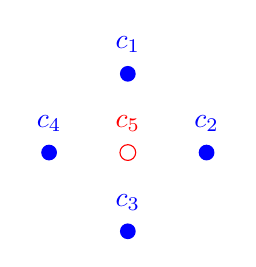
\begin{tikzpicture}[scale=1]
\fill[blue] (0,1) circle (0.1) node[above=4pt] {$c_1$};
\fill[blue] (1,0) circle (0.1) node[above=4pt] {$c_2$};
\fill[blue] (0,-1) circle (0.1) node[above=4pt] {$c_3$};
\fill[blue] (-1,0) circle (0.1) node[above=4pt] {$c_4$};
\draw[red] (0,0) circle (0.1) node[above=4pt] {$c_5$};
\end{tikzpicture}
\end{tabular}
\end{center}
~\\
{\bf Exercise:} show that no set of 5 points can be shattered by the Axis aligned rectangles class. Hint: note that the 3 points $(x_k,y_k)$, $(x_i,y_i)$, and $(x_{k'},y_{k'})$ can not be shattered if $x_k\leq x_i\leq x_{k'}$ and $y_k\leq y_i\leq y_{k'}$.


\subsubsection{Finite classes}
~\\{\bf Exercise:}
\begin{itemize}
\item Show that the VC dimension of a finite $\Hc$ is at most
$\log_2(|\Hc|)$.
\item  Assume $\Hc$ is finite. Show that there can be arbitrary gap between $VCdim(\Hc)$ and
  $\log_2(|\Hc|)$, namely, construct a finite hypothesis class $\Hc$ over some sample space $\X$ with $VCdim(\Hc) = \log_2(|\Hc|)$ 
  and another finite hypothesis class with $VCdim(\Hc)=1$.  
\end{itemize}

\subsubsection{Half-spaces through the origin}
Consider the sample space $\X = \reals^d$ and the hypothesis class of half-spaces through the origin
$\Hc = \{ \x \mapsto sign(\inner{\w,\x}): \w \in \reals^d\}$. 

~\\{\bf Exercise:}
\begin{itemize}
\item Show that $\{\e_1,\ldots,\e_d\}$ is shattered
\item Show that any $d+1$ points cannot be shattered (hint: consider the standard basis vectors...)
\item What is $VCdim(\Hc)$?
\end{itemize}

%\subsubsection{Classification trees}
%What is the VC-dimension of a full balanced classification tree with $b$
%levels?





\newpage
\part*{Lecture 5: PAC Theory of Statistical Learning, Part II}
\label{part:lecture_5}
\addcontentsline{toc}{part}{\nameref{part:lecture_5}}

\section{Recap of PAC Theory so far}


Make sure you've read the previous handout (PAC Part I). Recall that we are
developing a theory of ``learning from previous examples'' or ``generalizing
from previous examples'', which suggests a mathematical model for what it
means to learn, what is learnable and what isn't learnable, how to learn when
learning is possible, and what's the minimal number of training samples we need
to learn. All for {\bf supervised batch learning}.

\subsection*{Our framework and The Learning Game}



\paragraph{Framework.}

 Our task is to design a learning algorithm (a "learner"), which we denote by $\mathcal{A}$. For a given sample size $m$, $\mathcal{A}$  is a map from the training sample 
\[S=((x_1,y_1),..,(x_m,y_m)) \in (\X\times \Y)^m\]
where each $\mathbf{x}_i$
to an {\bf hypothesis class}  $\Hc\subset \Y^\X$. We write
$\Ac:(\X\times\Y)^m\to \Hc$ so that $\Ac:S\mapsto h_S\in\Hc$.

We're thinking of classification problems now, so in this lecture $\mathcal{Y}=\{\pm 1\}$, but everything here can be generalized.
The {\bf data generation model} we assume is probabilistic. 
We assume that there is an unknown distribution $\mathcal{D}$ over
$\mathcal{X}$.
 We assume that each sample - both in the training set and in the test set - is sampled
 according to $\mathcal{D}$ independently from any other sample before of after
 it. For the labels $y$, we assume a function $f:\mathcal{X}\to\mathcal{Y}$ such
 that for each sample $x\in\mathcal{X}$, the corresponding label is $y=f(x)$. We
 further assume (the {\bf ``realizability assumption''}) that $f$ is
 $\Dc$-almost-everywhere equal to some $h^*\in\Hc$, namely that $\Dc\left(
   \left\{ x\in\X\,|\, f(x)=h^*(x)  \right\}
 \right)=1$.
In particular, for our training data, we have $y_i = f(x_i)$ for $i=1,\ldots,m$. 
Finally, for a candidate prediction rule $h\in\Hc$ that our learner may produce,
we will measure the generalization performance of $h_S$ - how well it will perform on future unseen samples - by simply using the expected misclassification rate 
$$
L_{\D,f}(h) ~\eqdef~ \prob_{x \sim \D}[h(x) \neq f(x)] \,.
$$
Note that using this notation, the Realizability Assumtion can be written like
this: we assume that the labeling function $f:\X\to\Y $ is such that
$\exists h^*\in\Hc$ with $L_{\D,f}(h^*)=0$.


\paragraph{The Learning Game.} 
The definition of PAC-learnability is more easily understood by thinking about
supervised batch learning as a ``game between us and Nature''. 
Fix desired accuracy $\epsilon>0$ and confidence $\delta>0$. Fix
   an hypothesis class $\Hc \subset \Y^\X$. 
 We play a game against Nature, with random payoff.
  \begin{itemize}
    \item We choose a sample size $m$ and a learner $\Ac:(\X,\Y)^m \to \Hc$. 
    Both $m$ and $\Ac$ can depend on $(\epsilon,\delta)$.
       \item Nature knows our strategy, and, after us, chooses strategy that consists of a probability distribution $\D$ over $\X$, and a label function {\bf from the specified hypothesis class} $f\in\Hc$. 
     That is, Nature's strategy can depend on $\epsilon,\delta,\Hc$ specified, and also on the $m,\Ac$ we chose. 
    \item A sample $S$ of size $m$ is drawn according to $\D$ and is labeled
      according to $f$
    \item The sample $S$ is fed into $\Ac$ to produce a prediction rule
      $h_S=\Ac(S)$. Note that $h_S\in\Hc$.
    \item The payoff is $L_{\D,f}(h_S)$. It is random since $S$ is random and
      therefore $h_S$ is random.
    \item We are going to assume Nature is ``cruel'' and does her best to win.
      So we'll look for learners $\Ac$ that have a {\bf guaranteed maximal 
      loss} $L_{\D,f}(h)$ {\bf for any} strategy $\D,f$ that Nature might play.
      \item To determine if we were successful in the game, we play the game many many times 
      (both us and Nature play the same strategies, just the training samples drawn are different).
      We count and calculate the probability, over the random draws of training samples $S$, of the event
      $\{ S \sim \D^m \,\big |\,L_{\D,f}(h_S)\leq \epsilon \}$. If this probability is found to be 
      larger than $1-\delta$, that is, if 
      the learner $\Ac$ we chose was Probably Approximately correct with accuracy $\epsilon$ and confidence $\delta$ - against Nature's best strategy - {\bf we say that we've been successful (with regards to the parameters $\epsilon,\delta$) and hypothesis class $\Hc$}.
\end{itemize}

We saw that the definition of PAC learnability of an hypothesis class $\Hc$
(coming next) is equivalent to the following statement: We are able to ``win''
against Nature, for any $\delta,\epsilon>0$, regardless of how Nature plays.


\subsection*{PAC Learnability and Sample Complexity of an hypothesis class $\Hc$}

Slowly and gradually, in the last lecture we unpacked the following
definitions:

\begin{definition}
\begin{enumerate}
\item
A hypothesis class $\Hc$ is {\bf PAC Learnable} if there exists a function $\tilde{m}_\Hc : (0,1)^2 \to \N$ and a learning algorithm $\Ac$ with the following property:
For every $\epsilon,\delta \in (0,1)$ and for every distribution $\D$ over $\X$, and for every labeling function 
$f:\X\to\{\pm 1\}$ that satisfies $L_{\D,f}(h^*)=0$ for some $h^*\in\Hc$, when running the learning algorithm $\Ac$ on $m\ge \tilde{m}_\Hc(\epsilon,\delta)$ i.i.d. examples generated by $\D$ and labeled by $f$, the algorithm returns an hypothesis $h_S=\Ac(S)$ such that, with probability of at least $1-\delta$ (over the choice of the training samples), we have
$
L_{\D, f}(h_S) \le \epsilon
$. 
\item For a PAC learnable hypothesis class, we define the {\bf Sample Complexity} of $\Hc$ for specified $\epsilon,\delta$ as the minimal number of samples $\tilde{m}_\Hc(\epsilon,\delta)$ required for the definition to hold with respect to $\epsilon,\delta$. The Sample Complexity function of $\Hc$ is denoted $m_\Hc(0,1)^2\to\mathbb{N}$.
\end{enumerate}
\end{definition}

We defined a Probably Approximately Correct learner and saw that if an
hypothesis class $\Hc$ is PAC-learnable, this just means that for any $0<\epsilon,
\delta<1$ we are able to
find a Probably Approximately correct learner $\Ac$ with accuracy $\epsilon$ and
confidence $\delta$, regardless of $\D,f$ chosen by Nature. 


\section*{VC Dimension}

{\bf Definition:} Let $C\subset\X$ be a subset of the sample space and let $h:\X\to\Y$ be some hypothesis. 
We define the {\bf restriction} of $h$ to $C$, denoted $h_C:C\to\Y$, by $h_C(x)=h(x)$, for $x\in C$.
\\~\\
{\bf Crucial observation:} As long as $\Hc$ contains {\bf any} set $C$ of size
$2m$ with the property that $\{h_C\,|\,h\in\Hc\} = \Y^C$, then we cannot learn with a training sample of size $m$. It follows that the {\bf maximal size} of such a set $C$ in $\Hc$ is a {\bf critical quantity}: (i) it gives us a lower bound on $m_\Hc$, the minimal sample size needed, and (ii) if the maximal size is $\infty$, namely, if for any $m\in\mathbb{N} \X$ contains such as set $C$ with $|C|>m$, the $\Hc$ is not PAC-learnable!
\\~\\
This is the intuition behind the {\bf lower bound} in the Fundamental Theorem of Statistical
Learning: When trying to learn a function from an hypothesis class $\Hc$, the
{\bf minimal} number of samples needed to learn - using {\bf any} learner (not
just ERM) - is related to the maximal size of a set $C\subset \X$ with the
property that  $\{h_C\,|\,h\in\Hc\} = \Y^C$.

\subsection*{Formal Definition}

Let $C = \{x_1,\ldots,x_{|C|}\} \subset \X$ and let $\Hc_C$ be the restriction of $\Hc$ to $C$, namely,
 $\Hc_C = \{ h_C : h \in \Hc\}$.
 Observe that, always, $|\Hc_C|\leq 2^{|C|}$. The case where the upper bound is
 obtained is the one most interesting to us: 
We will say that $\Hc$ \textbf{shatters} $C$ if $|\Hc_C| =  2^{|C|}$.  
\begin{definition}
The VC dimension of the hypothesis class $Hc$ is defined as 
$$VCdim(\Hc) = \max\{ |C| ~:~ \Hc~\,\,\textrm{shatters}~\,\,C \}\,,$$
that is, the VC dimension is the maximal size of a set $C\subset \X$ such that
$\{h_C\,|\,h\in\Hc\} = \Y^C$.
\end{definition}
We interpret this as the maximal size of a set $C\subset X$ such that 
$\Hc$ gives no prior knowledge on label functions restricted to $C$.
\\
~\\ The {\bf lower bound} part of the Fundamental Theorem of Statistical
Learning gives an explicit connection between $VCdim(\Hc)$ (maximal size of a
subset of $X$ that is shuttered by $\Hc$) and the minimal
number of samples required to produce a PAC learner for $\Hc$ with confidence
$\delta$ and accuracy $\epsilon$ ($ m_\Hc(\epsilon,\delta)$ - the sample
complexity of $\Hc$ at $\epsilon,\delta$): there is a universal constant $C_1$
such that
\[
 C_1
    \frac{d + \log(1/\delta)}{\epsilon} \le m_\Hc(\epsilon,\delta)\]



\subsection*{Examples}
According to the above definition, in order to show that $VCdim(\Hc) = d$ we need to show that:
\begin{enumerate}
\item There exists a set $C$ of size $d$ which is shattered by $\Hc$.
\item Every set $C$ of size $d+1$ is not shattered by $\Hc$.
\end{enumerate}

\subsubsection*{Threshold class}
Consider first $\Hc_{th}$. The set $\{0\}$ is shattered by  $\Hc_{th}$ since $x=0$ can receive both the label 0 and 1, depending on the location of the threshold $\theta$. 

\begin{center}
 \includegraphics[width=0.5\textwidth,height=0.05\textheight]{ThresholdVC1.png}
\end{center}

In contrast to the above, no two points, $x_1$ and $x_2$ can be shattered because if $x_1 < x_2$ then $y_1 \leq y_2$ and therefore the pair of labels $y_1=1, y_2=0$ is forbidden.

\begin{center}
 \includegraphics[width=0.5\textwidth,height=0.05\textheight]{ThresholdVC2.png}
\end{center}

\subsubsection*{One-Interval}
Consider the \textbf{One-Interval} hypothesis class over the sample space 
$\X = \reals$. We define $\Hc = \{ h_{a,b} : a < b \in \reals\}$, where $h_{a,b}(x)=1$ if $x \in [a,b]$, and $h_{a,b}(x)=0$ otherwise.
Now, take for example the two points $\{0,1\}$.  We can place the interval over both, over any one of them, or outside $[0, 1]$. Therefore, $\{0,1\}$ is shattered. However, any three points cannot be shattered:
Let $x_1 < x_2 < x_3$, then no single interval can cover $x_1$ and $x_3$ without containing also $x_2$ and therefore the labeling $y_1=1, y_2=0, y_3=1$ is forbidden.

\subsection*{Exercises to help you understand the definition of VC-dimension}

Make sure to solve all these exercises. They will help you understand the
definition of VC-dimension.

\subsubsection*{Axis aligned rectangles}
Consider the \textbf{Axis aligned rectangles} hypothesis class over the sample space 
$\X = \reals^2$. We define $\Hc = \{h_{(a_1,  a_2, b_1 , b_2)}: a_1 < a_2 ~\text{and}~  b_1 < b_2 \}$, 
where $ h_{(a_1, a_2, b_1 , b_2)}(x_1,x_2) = 1$ if $x_1 \in [a_1,a_2]$, and $x_2 \in [b_1,b_2]$, and  $ h_{(a_1, a_2, b_1 , b_2)}(x_1,x_2) = 0$ otherwise. (Convince yourself that a function in this hypothesis class is an indicator of a finite open rectangle aligned with the canonical basis of $\reals^2$.)

\vspace{9mm}

Verify that:
\begin{center}
\begin{tabular}{lr}
Shattered & Not Shattered \\
\begin{tikzpicture}[scale=1]
\fill[blue] (0,1) circle (0.1);
\fill[blue] (1,0) circle (0.1);
\fill[blue] (0,-1) circle (0.1);
\fill[blue] (-1,0) circle (0.1);
\end{tikzpicture} & \hspace{2cm}
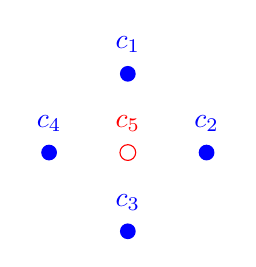
\begin{tikzpicture}[scale=1]
\fill[blue] (0,1) circle (0.1) node[above=4pt] {$c_1$};
\fill[blue] (1,0) circle (0.1) node[above=4pt] {$c_2$};
\fill[blue] (0,-1) circle (0.1) node[above=4pt] {$c_3$};
\fill[blue] (-1,0) circle (0.1) node[above=4pt] {$c_4$};
\draw[red] (0,0) circle (0.1) node[above=4pt] {$c_5$};
\end{tikzpicture}
\end{tabular}
\end{center}
~\\
{\bf Exercise:} show that no set of 5 points can be shattered by the Axis aligned rectangles class. Hint: note that the 3 points $(x_k,y_k)$, $(x_i,y_i)$, and $(x_{k'},y_{k'})$ can not be shattered if $x_k\leq x_i\leq x_{k'}$ and $y_k\leq y_i\leq y_{k'}$.


\subsubsection*{Finite classes}
~\\{\bf Exercise:}
\begin{itemize}
\item Show that the VC dimension of a finite $\Hc$ is at most
$\log_2(|\Hc|)$.
\item  Assume $\Hc$ is finite. Show that there can be arbitrary gap between $VCdim(\Hc)$ and
  $\log_2(|\Hc|)$, namely, construct a finite hypothesis class $\Hc$ over some sample space $\X$ with $VCdim(\Hc) = \log_2(|\Hc|)$ 
  and another finite hypothesis class with $VCdim(\Hc)=1$.  
\end{itemize}

\subsubsection*{Half-spaces through the origin}
Consider the sample space $\X = \reals^d$ and the hypothesis class of half-spaces through the origin
$\Hc = \{ \x \mapsto sign(\inner{\w,\x}): \w \in \reals^d\}$. 

~\\{\bf Exercise:}
\begin{itemize}
\item Show that $\{\e_1,\ldots,\e_d\}$ is shattered
\item Show that any $d+1$ points cannot be shattered (hint: consider the standard basis vectors...)
\item What is $VCdim(\Hc)$?
\end{itemize}

%\subsubsection{Classification trees}
%What is the VC-dimension of a full balanced classification tree with $b$
%levels?







\section{Finite Hypothesis Classes are PAC learnable}

We talked about finite hypothesis classes in the previous lecture, and stated a
theorem whereby finite hypothesis classes are PAC learnable, but did not
prove it. Let's recall the details and prove the theorem.

We recall that a finite hypothesis classes can be huge: for example, take $\Hc$ is all the functions from $\X$ to $\Y$ that can be implemented using a Python program of length at most $b$, for $b$ fixed and large. Or, take $\Hc$ to be all the functions from $\X$ to $\Y$ where  $|\X|$ and $|\Y|$ are finite.

\subsubsection{Empirical Risk Minimization}

It turns out that {\bf there is a simple learner that is always successful on finite hypothesis classes} (and on many other hypothesis classes as we will see later).

The idea behind this amazing learning is very simple and natural: try to be as correct as possible on the training data!

Formally, given  a training set $S = (x_1,y_1),\ldots,(x_m,y_m)$ we define the {\bf empirical risk} of a candidate prediction rule $h\in\Hc$ by
$$L_S(h) = \frac{1}{m} |\{i : h(x_i)  \neq y_i\}|\,.$$

Our amazing learning algorithm is simple: on a training sample $S$, it returns $h \in \Hc$ that {\bf minimizes the empirical risk $L_S(h)$.} In other words,
\[
\Ac_{ERM} : S \mapsto \text{argmin}_{h\in\Hc} L_S(h) = \frac{1}{m} \,.
\]
The minimum may not be unique, in which case the algorithm returns one of the minimizers. Our amazing learner is therefore called \textbf{Empirical Risk Minimization (ERM)} learner. We give this important learner its own special notation and denote it by $ERM_\Hc$ instead of $Ac_{ERM}$.

But wait, how do we know that there is a minimum?  Note that $L_S(h)\geq 0$, and we are minimizing over a finite class, so there is a minimum. In fact, under the assumption that Nature plays $f\in\Hc$, we know that for any training sample $S$,  $L_S(f) = 0$ for the particular labeling function that Nature chose. So that the lower bound $0$ is achievable. In other words, under our assumption that $f\in\Hc$, the ERM learner will always return a rule  $h$ with $y_i = h(x_i)$ for $i=1,\ldots,m$. 
Such a rule is called \textbf{Consistent} - it is consistent with the training sample. 


\subsubsection{Learning Finite Classes}

Our main observation concerning finite classes is simple: a {\bf finite} hypothesis
class $\Hc\subset\Y^\X$ is PAC-learnable, using the ERM rule,
with sample complexity at most 
$\log(|\Hc|/\delta)/\epsilon$.

\begin{theorem}
  Fix $0< \epsilon,\delta <1$. If \[m \ge \frac{\log(|\Hc|/\delta)}{\epsilon}\] 
  then for every $\D$ over $\X$ and every $f$ such that $\exists h^*\in\Hc$ with
  $L_{D,f}(H^*)=0$, with probability of at least $1-\delta$ (over the choice of $S$ of size $m$), $L_{\D,f}(ERM_\Hc(S)) \le \epsilon$.
\end{theorem}

In words, the theorem states that a finite hypothesis class $\Hc$ is PAC
learnable with sample complexity $m_\Hc(\epsilon,\delta)\leq
\frac{\log(|\Hc|/\delta)}{\epsilon}$.
The figures below explain schematically the relation between the accuracy, confidence and the sample size for finite classes, as implied by the above theorem.

% \begin{figure}[h!]
% \centering\includegraphics[scale=0.8]{connection_m_eps_delta.eps}
% \end{figure}


  \begin{figure}[h!]
 \centering\includegraphics[scale=0.8]{connection_m_eps_delta_finite4.eps}
  \end{figure}


  \begin{figure}[h!]
 \centering\includegraphics[scale=0.8]{connection_m_eps_delta_finite2.eps}
 \end{figure}


  \begin{figure}[h!]
 \centering\includegraphics[scale=0.8]{connection_m_eps_delta_finite3.eps}
 \end{figure}

Let us prove the theorem in full (more details can be found in \textit{Understanding Machine Learning} Ch. 2.3.1). For each $S$ our algorithm chooses a hypothesis $ERM_{\Hc}(S)$
Let $\Hc_B$ be the set of "bad" hypotheses,
 \[ \Hc_B = \{h \in \Hc : L_{\D,f}(h) > \epsilon\} \]
and let $S|_x = (x_1,\ldots,x_m)$ be the instances of the training set. We would like to prove:
\[
\D^m(\{ S|_x : ERM_{\Hc}(S)\in \Hc_B \})  \le \delta
\]

Let us denote by $M$ the set of "misleading" samples,
\[M = \{S|_x : \exists h \in \Hc_B, L_S(h)=0\} \]
%
that is, for every input sample $S$ in $M$ there exists an $h$ that in spite of being perfectly correct on that sample, and therefore \textit{could be} chosen by the ERM algorithm as a possible output for that input, its global error is larger than $\epsilon$. In particular, all the $S$'s in the set $\{ S|_x : ERM_{\Hc}(S)\in \Hc_B \}$ belong to $M$ because these are the samples for which our \textit{specific} algorithm chooses a "bad" $h$ (that is, one with $L_{\D,f}(h) > \epsilon$, which means it is in $\Hc$) and being an ERM algorithm, the $h$ it outputs must satisfy $L_S(h)=0$. Therefore:
%
\[\{S|_x : L_{\D,f}(ERM_\Hc(S)) > \epsilon\} \subseteq M \,.\]
We can rearrange the samples in  $M$ according to the $h$'s they share by writing $M$ as:
\[ M = \bigcup_{h \in \Hc_B} \{ S|_x : L_S(h) = 0 \}\]
In this representation, samples in $M$ which share several $h$'s will be counted more than once but since $M$ is a set, this has no effect.
Combining the last two relations we have
\[\{S|_x : L_{\D,f}(ERM_\Hc(S)) > \epsilon\} \subseteq M \]
and using the \textbf{Union Bound}, that is, the fact that for any two sets $A,B$ and a distribution $\D$ we have $\D(A \cup B) \le \D(A) + \D(B) ~$, we get
$$\D^m(\{ S|_x : L_{\D,f}(ERM_\Hc(S)) > \epsilon \}) \le \sum_{h \in \Hc_B} \D^m( \{ S|_x : L_S(h) = 0 \} )\,.$$
Given an $h$, $ \D^m( \{ S|_x : L_S(h) = 0 \}$ is the probability to pull a sample over which $h$ is perfectly correct (has the right labels for all $x_i$'s). 
Since the  $x_i$'s are drawn independently, this probability equals the probability that $h$ will be correct for each of the $x_i$'s separately. 
But the probability that $h$ will be \textit{incorrect} for a random $x$ is exactly $L_{\D,f}(h)$. So the probability that $h$ will be correct for $m$ such $x$'s is $(1-L_{\D,f}(h))^m$. 
We therefore have, for any $h$,
\[ \D^m( \{ S|_x : L_S(h) = 0 \} ) = (1-L_{\D,f}(h))^m \quad \forall h \,.\]
In particular, if $h \in \Hc_B$ then $L_{\D,f}(h) > \epsilon$ and therefore
\[ \D^m( \{ S|_x : L_S(h) = 0 \} ) < (1-\epsilon)^m \quad \forall h \in \Hc_B \,.\]
Substituting this bound above we obtain
\[ \D^m(\{ S|_x : L_{\D,f}(ERM_\Hc(S)) > \epsilon \}) \le \sum_{h \in \Hc_B} (1-\epsilon)^m < |\Hc_B|\,(1-\epsilon)^m  \le  |\Hc|\,(1-\epsilon)^m \,.\]

Finally, using $1-\epsilon \le e^{-\epsilon}$ we conclude:
\[ \D^m(\{ S|_x : L_{\D,f}(ERM_\Hc(S)) > \epsilon \}) ~<~ |\Hc|\,e^{-\epsilon\,m} \,.\]

The right-hand side would be $\le \delta$ if $m \ge
\frac{\log(|\Hc|/\delta)}{\epsilon}$ and therefore we are done. $\blacksquare$

\vspace{5mm}

The figure below illustrates the use of the union bound. Each point is a possible sample $S|_x$. Each colored oval
  represents misleading samples for some $h \in \Hc_B$. The probability
  mass of each such oval is at most $(1-\epsilon)^{m}$. But, the algorithm
  might err if it samples $S|_x$ from any of these ovals.

\begin{center}
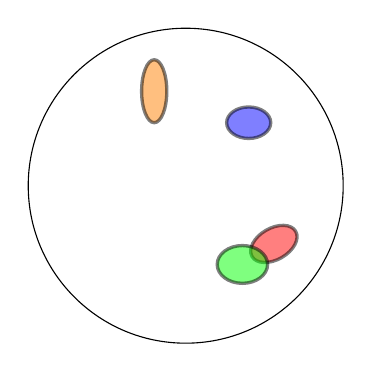
\begin{tikzpicture}[scale=0.4]
\draw (0,0) circle (5);
\filldraw[very thick,color=black,fill=blue,opacity=.5] (2,2) ellipse (0.7 and 0.5);
\filldraw[very thick,color=black,fill=orange,opacity=.5] (-1,3) ellipse (0.4 and 1);
\filldraw[very thick,color=black,fill=red,rotate=30,opacity=.5] (1.5,-3) ellipse (0.8 and 0.5);
\filldraw[very thick,color=black,fill=green,opacity=.5] (1.8,-2.5) ellipse (0.8 and 0.6);
\end{tikzpicture}
\end{center}

\vspace{5mm}

To summarize this section, we have shown the following:
{\bf A finite hypothesis class $\Hc$ is PAC learnable using the ERM learning algorithm, and has a sample complexity  $m_\Hc(\epsilon,\delta)\leq \log(|\Hc|/\delta)/\epsilon$ samples.}

%So, given $\epsilon,\delta \in (0,1)$, all that the learning algorithm needs is to be consistent with the sample (to be an ERM) while the sample size $m$ should satisfy $m\ge m_\Hc(\epsilon,\delta)= \frac{\log(|\Hc|/\delta)}{\epsilon}$.



\section{The Fundamental Theorem of Statistical Learning}

We worked hard to understand the two fundamental definitions above: VC-Learnability (and sample complexity) of an hypothesis class, and VC-dimension of an hypothesis class. 
\\~\\
Along the way, we saw some connections between these two definitions:
\begin{itemize}
    \item We saw that a finite hypothesis class is PAC-learnable (using the ERM learner)
    with sample complexity \[m_\Hc(\epsilon,\delta)\leq \frac{\log(|\Hc|) + \log(1/\delta)}{\epsilon} \]
    and also that in this case $VCdim(\Hc)\leq \log(|\Hc|)$. Somehow it seems that $VCdim(\Hc)$ is related to an upper bound on $\Hc$ for finite hypothesis classes.
    \item We saw, using a loose argument (the "proof" of No Free Lunch), that $VCdim(\Hc)$ also gives a {\bf lower bound} on the sample complexity $m_\Hc$ of an hypothesis class $\Hc$, and that if $VCdim(\Hc)$ is infinite, that class is not PAC-Learnable. 
\end{itemize}

The surprising, shocking, wonderful truth is that VC-dimension gives a complete and full characterization of PAC-learnabilty and sample complexity of an hypothesis class, and gives a decisive answer to all the questions we posed at various stages along the way (such as which classes are PAC-learnable, with what sample complexity, and with what algorithm, and is there an algorithm that uses the minimal possible sample size.)

The Fundamental Theorem of Statistical Learning states as follows:
\begin{itemize}

\item The PAC-lernability of an hypothesis class is characterized by the \textbf{VC dimension}, a combinatorial property of the class that denotes the maximal size of a sample that can be shuttered by the class.  The characterization is as follows: an hypothesis class is PAC-learnable {\bf if and only if} its VC-dimension is finite.
\item When $VCdim(\Hc)$ is finite (so that $\Hc$ is PAC-learnable and we can ask about its sample complexity), its sample complexity is basically 
\[
m_H(\epsilon,\delta) \sim \frac{VCdim(\Hc)+\log(1/\delta)}{\epsilon}
\]
up to come constants. 
\item The ERM learning rule is a generic (near) optimal learner, in the sense that when a hypothesis class is PAC-learnable, ERM using 
\[
m(\epsilon,\delta) \sim  \frac{VCdim(\Hc)\log(1/\epsilon)+\log(1/\delta)}{\epsilon}
\]
is a Probably Approximately correct learner with accuracy $\epsilon$ and confidence $\delta$.
\end{itemize}

The formal statement of the theorem is as follows: (see   Understanding Machine Learning book, ch. 6.6)
	

  \begin{theorem}[The Fundamental Theorem of Statistical
    Learning] 
    Let $\Hc$ be a hypothesis class of
    binary classifiers with VC-dimension $d\leq \infty$. 
    Then, $\Hc$ is PAC-learnable if and only if $d<\infty$. In this case: (1) there
    there are absolute constants $C_1,C_2$
    such that the sample complexity of $\Hc$ satisfies \[ C_1
    \frac{d + \log(1/\delta)}{\epsilon} \le m_\Hc(\epsilon,\delta) \le
    C_2 \frac{d \log(1/\epsilon) + \log(1/\delta)}{\epsilon} \]
(2) Furthermore, the upper bound on sample complexity is achieved by the ERM learner.
  \end{theorem}

  We already saw the intuition behind the lower bound - how the VC-dimension
  $VCdim(\Hc)$ is related to the {\bf minimal} number of training samples needed
  to PAC-learn the hypothesis class $\Hc$ - using {\bf any} learning algorithm.
\\~\\
To understand the upper bound, we need to understand 
how is it that the ERM learner is a {\bf generic
learning algorithm} that is able to PAC-learn $\Hc$ with a training sample size
again related to the VC-dimension $VCdim(\Hc)$.
\\~\\
Before we discuss the upper bound, let us extend our theoretic framework and
make it much more flexible and realistic.



  \section{Agnostic PAC: Extending our theoretical framework}

  The theoretical framework we developed is not so satisfying, and is
  not such a great theoretical model for ``real'' learning problems, for a few
  reasons:
  \begin{itemize}
    \item {\bf It doesn't model noisy labels.} We have no model for measurement errors. In practice, sometimes even
      though the label for some $\x\in\X$ ``should'' have been $1$ (say), it can
      be measured as $-1$ due to measurement mistake, noise, etc. We want our
      framework to allow for the fact that we may, with low probability, observe the point $x\in\X$
      twice, and get two different labels - namely, observe $(x,+1)$ and later
	sample again and observe $(x,-1)$ - due to noise. 
      \item {\bf The realizability assumption is  unrealistic.} We define
        the hypothesis class.  It is unrealistic to restrict Nature to choose
	from the hypothesis class that we defined. Nature will do as she likes.
      \item {\bf Limited to misclassification loss.} In our framework, we could
	only
	measure the classifier performance using the misclassification loss
	(otherwise known as the $0-1$ loss). We would like to be able to measure
	performance using any loss function we like.
  \end{itemize}

  We now introduce an improved theoretical framework, sometimes know as {\bf
  Agnostic PAC}. It improves on the PAC learning framework and  solves the
  problems above: (i) it allows 
  measurement noise,  (ii) it removes the realizability assumption, and (iii) it
  allow us to specify any loss function. The good
  thing is, as we mention below, the fundamental theorem of statistical learning
  holds in the Agnostic PAC framework as well.


  \subsection{Moving from a probability distribution over $\X$ to a joint
  probability distribution over $\X\times\Y$}

%    \label{D:def} [UML Section 3.2.1]
  Our first step will be to change the probability distribution $\Dc$. For far,
  $\Dc$ was a probability distribution over the sample space $\X$, and the
  labels were determined - deterministically - using the labeling function $f$.
  In our upgraded framework, $\Dc$ will be a probability distribution over
  $\X\times \Y$. This means that when we draw a new random example $(x,y)$ - whether for
  the training sample $S$ or as a test sample - there is randomness in {\bf
  both} $x$ and $y$, and, crucially, it's a {\bf joint} randomness. 
  \\~\\
  We can factor $\Dc$ in two ways, conditioning on $x$ or on $y$. Both are useful for our understanding.
  Let $(X,Y)$ be a random variable taking valued in $\X\times \Y$ whose
  distribution is $\Dc$. 
\begin{itemize}
  \item $\prob(X=x,Y=y)=\prob(X=x)\prob(Y=y|X=x)$. From this perspective, this is a direct
    generalization of our previous framework, where $x$ was random and $y=f(x)$.
    Indeed, we draw $x$ from the marginal distribution with probability
    $\prob(X=x)$ - as we did in the previous framework. We then choose a corresponding 
    label according to the conditional probability $\prob(Y=y|X=x)$. Since the
    marginal random variable $Y$ is a Bernoulli random variable, this means
    there's a function $p:\X\to[0,1]$ such that $\prob(Y=+1|X=x)=p(x)$, namely,
    choosing the label for $x$ is a coin flip with probability $p(x)$. If
    $p(x)=0$ or $p(x)=1$ for some $x$, the label is deterministic and we are
    back to the ``label function'' $f$. But for other values of $p(x)$, whereas
    before the label depended deterministically on $x$, now it is random.
    This models {\bf measurement noise} - the fact that there may be noise in
    the labels, and that the distribution of the noise may change from $x$ to $x$. 
    (This is the perspective of the Logistic Regression classifier you saw in
    the classification lecture, for example. There, we didn't pay attention a
  distribution on $x$ - just assumed the samples are given - and tried to
estimate the conditional probability $\prob(Y=+1|X=x)=p(x)$.)
  \item $\prob(X=x,Y=y)=\prob(Y=y)\prob(X=x|Y=y)$. For this perspective, we
    first draw the label according to a ``coin flip'' -  a Bernoulli random
    variable. Then, each class has its own distribution for the samples $x$. We
    draw the label $x$ from $\prob(X=x|Y=+1)$ or from $\prob(X=x|Y=-1)$, according
    to the label $y$ chosen. (This is the perspective of the LDA classifier you
    saw in homework, for example.) 
\end{itemize}
  
  
\paragraph{Exercise.} Let $\tilde{\D}$ be a distribution on $X$ alone, and let
$f:\X\to\Y$ be a labeling function. Construct an equivalent joint distribution
$\D$ on $\X\times\Y$ such that the random variable $(X,f(X))$, where
$X\sim\tilde{\D}$, has the same distribution over $\X\times\Y$ as $(X,Y)\sim\D$. 
%
\\~\\
How shall we define the loss, when $\Dc$ is a distribution over $\X\times \Y$?
It's simple. Staying (for now) with the misclassification loss, we just define,
for a hypothesis $h:\Xc\to\Yc$,
    \begin{eqnarray} \label{L:def}
        L_\Dc(h) := \Prob_{(x,y)\sim\Dc}\left\{ h(x)\neq y \right\}
        \equiv \Dc\left\{ (x,y)\,|\, h(x)\neq y \right\}
    \end{eqnarray}
    ~\\
    Notice we no longer have a ``ground truth'' labeling function $f$. The
    closest thing we have to $f$  is the conditional probability
    $\prob(Y=y|X=x)$.




\subsection{Removing the realizability assumption}

Recall that in the deterministic labeling case, under the realizability
assumption, we could reach zero generalization error:
\[
    \min_{h\in\Hc} L_{\Dc,f}(h) = L_{\Dc,f}(f)=0\,.
\]
However, in the random labeling case, there is no ``ground truth'' labeling function $f:\Xc\to\Yc$, so
that the realizability assumption no longer makes sense. Due to the measurement
noise, we may no longer be able to reach $0$ generalization loss. This means we
have to change the definition of {\bf accuracy}: we expect the learning
algorithm to output a rule which has generalization loss {\bf at most $\epsilon$
larger than the
minimal possible loss} $\min_{h\in\Hc} L_\Dc(h)$. 
But wait, does a minimum exist? What can we say about this minimum?

%[Bayes optimal predictor - UML section 3.2.1]

\paragraph{Definition: Bayes optimal predictor}
In the recitation you saw the following definition.
    For a given distribution $\Dc$ on $\Xc\times \Yc$ define the {\em Bayes
    optimal predictor} for $\Dc$ by 
    \[
        f_\Dc(x) = 
        \begin{cases}
            1 & \Prob(y=1|x)\geq 1/2\\
            0 & otherwise
        \end{cases}
    \]
~\\
Note that $f_\Dc:\X\to\Y$ is a rule (an hypothesis). However it depends on
$\Dc$, which, according to the rules of the game, we don't know. So $f_\Dc$ is
what is known as an {\bf Oracle Quantity} - if we had an oracle telling us
$\Dc$, then we could classify with $f_\Dc$. Oracle quantities, like this one,
are used to compare the loss of any other rule to the loss of the {\bf best
possible} rule. 
\\~\\
In homework you solved the following
{\bf Exercise.} The Bayes optimal predictor has the best possible generalization
error: 
$ \forall g:\Xc\to\Yc  \,\,,\,\, L_\Dc(f_\Dc)\leq L_\Dc(g) $. 
\\~\\
It follows that for any hypothesis class $\Hc\subset \Y^\X$,
\[
  L_\Dc(f_\Dc) = \min_{h\in \Y^\X} L_\Dc(h)  \leq \min_{h\in\Hc} L_\Dc(h)
\]
and so  $\{L_\Dc(h)\,|\, h\in\Hc\}$ is bounded from below and, glossing over the
difference between minimum and infimum, we can write $\min_{h\in\Hc} L_\Dc(h)$.
~\\
\paragraph{Definition:}
Let $\epsilon>0$.
We say that a rule $h\in\Hc$ is Approximately correct with accuracy $\epsilon$
with respect to the distribution $\Dc$ on $\X\times \Y$ if 
\[
   L_\Dc(h) \leq  \min_{h'\in\Hc} L_\Dc(h') + \epsilon\,,
\]
namely, if $L_\Dc(h)$  is at most $\epsilon$ away from the best possible loss
achievable by {\bf any} hypothesis in $\Hc$. We note again that, in our previous
framework, under the
realizability assumption, the minimal loss is simply $0$ since we {\bf assumed}
the existence of some $h'\in\Hc$ with $L_\Dc(h')=0$.
\\~\\
So, we got rid of the realizability assumption: we no longer assume that Nature
plays a labeling function in the chosen hypothesis class $\Hc$. In fact, we no
longer have a labeling function at all! Nature's strategy just consists of the joint
distribution $\D$ over $\X\times \Y$.

\subsection{Introducing a general loss function}

So we achieved two of the three improvements we wanted: we allow measurement
noise in the labels, and we got rid of the realizability assumption. 
Our last improvement is to allow a general loss function.
% [UML section 3.2.2]
 \paragraph{Definition:  general loss function.}
 A {\bf loss function} is a function $\ell:\Hc \times Z\to[0,\infty)$, where 
 $Z = \X\times\Y$.
For  $z=(x,y)$, we simplify the notation and, instead of the cumbersome notation
$\ell(h,z)$, we simply write  $\ell(h(x),y)$.
\\~\\
We already know well the most common example for classification loss - the
misclassification loss, also known as the  {\bf 0-1 loss}.
\[
    \ell_{0,1}(h,(x,y)):=
    \begin{cases}
        1 & h(x)\neq y\\
        0 & h(x)= y
\end{cases}\,.
\]
\\~\\
Indeed the loss we work with $L_\Dc(h)$ from \eqref{L:def} above can we written
as 
\[
    L_\Dc(h) \equiv \E_\Dc [\ell_{0-1}(h,(x,y))]
\]
where here and below $\E_\Dc[\cdot]$ denotes the expected value according to
$(x,y)\sim \Dc$. 

From here on we will assume a general loss function $\ell$, but will often
have in mind $\ell_{0,1}$.

\paragraph{Definition: generalization loss induced by a general loss function.}
 For a distribution $\Dc$ on $\X\times\Y$ and a loss $\ell:\Hc\times Z\to[0,\infty)$
 (where again $Z=\X\times \Y$) we
 extend Definition \ref{D:def} and define the loss of a rule (hypothesis)
 $h:\X\to\Y$ with respect to $\D$ and $\ell$ as
 \begin{eqnarray*}
     L_\Dc(h) := \E_{z\sim\Dc}[\ell(h,z)]
 \end{eqnarray*}
 where $Z=\Xc\times\Yc$ and $z=(x,y)\in Z$.
\\~\\
How shall we define {\bf accuracy} with respect to a general loss induced by a
general loss function? The definition above (for $0-1$ loss) generalizes
naturally and easily:
%
\paragraph{Definition:}
Let $\epsilon>0$.
We say that a rule $h\in\Hc$ is Approximately correct with accuracy $\epsilon$
with respect to the distribution $\Dc$ on $\X\times \Y$, the loss function
$\ell:\Hc\times (\X \times\Y)\to[0,\infty)$ and the hypothesis class $\Hc$ 
if 
\[
  L_\Dc(h) \leq \min_{h'\in\Hc} L_\Dc(h') + \epsilon\,.
\]
Note that now accuracy must be defined with respect to an hypothesis class
$\Hc$.



 \section{Agnostic-PAC learnability}
 Our new framework is called Agnostic-PAC.
 We are now ready to define Agnostic-PAC Learnability of a hypothesis class.

\subsection{Probably Approximately correct learner - in the new framework.}

\paragraph{Exercise.} Define - rigorously - what it means for $h:\X\to\Y$ to be
an Agnostic Probably Approximately correct learner with accuracy $\epsilon$ and confidence
$\delta$, with respect to a loss function $\ell$, hypothesis class $\Hc$ and a
distribution $\Dc$ on $\X\times\Y$.
~\\
\paragraph{Exercise.} Let $X$ be a sample space, $\Hc\subset \Y^\X$ an
hypothesis class, and let $\ell_{0-1}$ be the $0-1$ loss function. Let
$0<\epsilon,\delta<1$. Assume that
$h\in\Hc$ is an Agnostic Probably Approximately correct learner (with accuracy $\epsilon$ and confidence
$\delta$), with  respect to $\ell_{0-1}$, $\Hc$. Show that it follows
that $h$ is a Probably Approximately Correct learner (with accuracy $\epsilon$ and confidence
$\delta$)


\subsection{Agnostic-PAC learnability}

\begin{definition} \label{apac:def}
    A hypothesis class $\Hc$ is Agnostic-PAC learnable with respect to
    loss $\ell:\Hc\times (\X\times \Y)\to[0,\infty)$ if there exists a function
    $\tilde{m}_\Hc:(0,1)^2\to\N$  and a
a learning algorithm $\Ac:(\Xc\times\Yc)^m\to\Hc$
with the following property: For every $(\epsilon,\delta)\in (0, 1)$ 
for every distribution $\Dc$ over $\Xc\times \Yc$ , for any $m\geq \tilde{m}_\Hc(\varepsilon,\delta)$ 
\[
    \Dc^m\{ S_m \,|\, L_{\Dc}(h_S) \leq \min_{h'\in\Hc} L_\Dc(h) + \varepsilon\} \geq 1-\delta
\]
where $S_m=\left( x_1,y_1 \right),\ldots \left( x_m,y_m \right)$ is sampled
i.i.d according to $\Dc$, and $h_S=\Ac(S)$.
\end{definition}
~\\
Note that,  as before, we abused notation and wrote $\Ac$ for the entire sequence
of learners
$A_m:(\Xc\times\Yc)^m\to\Hc$, one for each possible sample size $m$.



\paragraph{Exercise.} To make sure you understand the definition, prove the
following rigorously: if 
an hypothesis class $\Hc$ is Agnostic-PAC learnable with respect to $\ell_{0-1}$, then it is PAC-learnable. 

\paragraph{The Learning Game.} 
To help us understand the definition of Agnostic-PAC learnability, let us write
the ``learning game'' in the Agnostic PAC framework.
\\~\\
Fix desired accuracy $\epsilon>0$ and confidence $\delta>0$. Fix
an hypothesis class $\Hc \subset \Y^\X$ and a loss function $\ell$.
 We play a game against Nature, with random payoff.
  \begin{itemize}
    \item We choose a sample size $m$ and a learner $\Ac:(\X,\Y)^m \to \Hc$. 
    Both $m$ and $\Ac$ can depend on $(\epsilon,\delta)$.
       \item Nature knows our strategy, and, after us, chooses strategy that
         consists of a probability distribution $\D$ over $\X\times \Y$.
     (Nature's strategy can depend on $\epsilon,\delta,\Hc$ specified, and also
     on the $m,\Ac$ we chose. )
   \item A sample $S\in(\X\times\Y)^m$ of size $m$ is drawn according to $\D$.
    \item The sample $S$ is fed into $\Ac$ to produce a prediction rule
      $h_S=\Ac(S)$. Note that $h_S\in\Hc$.
    \item The payoff is $L_{\D}(h_S)=\mathbb{E}_{(x,y)\sim\D}\ell(h,(x,y))$. It is random since $S$ is random and
      therefore $h_S$ is random.
    \item We are going to assume Nature is ``cruel'' and does her best to win.
      So we'll look for learners $\Ac$ that have a {\bf guaranteed maximal 
      loss} $L_{\D}(h)$ {\bf for any} strategy $\D,f$ that Nature might play.
      \item To determine if we were successful in the game, we play the game many many times 
      (both us and Nature play the same strategies, just the training samples drawn are different).
      We count and calculate the probability, over the random draws of training samples $S$, of the event
      $\{ S \sim \D^m \,\big |\,L_{\D}(h_S)\leq \min_{h'\in\Hc}L_\D(h') +
      \epsilon \}$. (To do this we assume knowledge of the ``Oracle quantity''
        $\min_{h'\in\Hc}L_\D(h')$ - the best possible loss of any rule in
      $\Hc$.) If this probability is found to be 
      larger than $1-\delta$, that is, if 
      the learner $\Ac$ we chose was Probably Approximately correct with accuracy $\epsilon$ and confidence $\delta$ - against Nature's best strategy - {\bf we say that we've been successful (with regards to the parameters $\epsilon,\delta$) and hypothesis class $\Hc$}.
\end{itemize}


\subsection{PAC learnability is equivalent to Agnostic-PAC learnability}

While we will not prove this, it turns out that moving to the more general
framework of Agnostic-PAC didn't change anything:
\paragraph{Theorem.} Let $X$ be a sample space and $\Hc\subset \Y^\X$ an
hypothesis class. Then $\Hc$ is PAC-Learnable if and only if it is Agnostic-PAC
learnable. 


\section{Back to the Fundamental Theorem of Statistical Learning}


\subsection{Empirical Risk Minimization strikes again}

Recall that in our previous framework, in the realizable case, the Empirical Risk Minimization (ERM) learner was
defined as any $h\in\Hc$ consistent with the training set 
$S=(x_1,y_1),\ldots,(x_m,y_m)$. In our more general case we redefine ERM as 
{\bf any} minimizer of the empirical risk.

\paragraph{Definition: Empirical Risk} with respect to a general loss function.
Let $h:\X\to\Y$ be a rule (hypothesis). We define the empirical risk of $h$ with
respect to the loss function $\ell$ and sample $S=(x_1,y_1),\ldots,(x_m,y_m)$ by 
\begin{eqnarray}
    L_S(h) := \frac{1}{m}\sum_{i=1}^m \ell(h,z_i)
\end{eqnarray}
where $z_i=(x_i,y_i)$.
\\~\\
\paragraph{Definition: ERM learner in the Agnostic-PAC framework.} The ERM learning algorithm, in our upgraded
framework, is define as
\[
\Ac_{ERM} : S \mapsto \text{argmin}_{h\in\Hc} L_S(h).
\]
Note - as before - that the ERM rule may not be unique. There may be many
hypotheses in $\Hc$ that achieve the minimum $ \text{min}_{h\in\Hc} L_S(h)$.

\subsection{ERM makes sense due to WLLN}

Now, recall the {\bf Weak Law of Large Numbers} (WLLN):
\begin{itemize}
     \item  If $X_i$ are i.i.d
       random variables and $\mu=\mathbb{E}(X_i)$, then
       \[
	 \lim_{m\to\infty} \frac{1}{m}\sum_{i=1}^m X_i = \mu
       \]
       where the convergence is {\bf in probability}
     \item Namely, for any $\delta>0$
\[
  \lim_{m\to\infty} \prob\left\{ \Big|   \frac{1}{m}\sum_{i=1}^m X_i - \mu \Big|>\delta \right\} =0
\]
\item Namely, for any $\delta>0$ there is $m_0\in\mathbb{N}$ such that for $m>m_0$,
\[
  \prob\left\{ \Big|   \frac{1}{m}\sum_{i=1}^m X_i - \mu \Big|>\delta \right\} <
  \epsilon\,.
\]
   \end{itemize}
~\\
Observe now that for any $h$ we have $\E_\Dc L_S(h) = L_\Dc(h)$. 
\begin{itemize}
	\item By WLLN, when $S$ is i.i.d sample of size $m$, 
	  $\lim_{m\to\infty} L_S(h) = L_\Dc(h)$, in probability
	\item Therefore for any
 $\delta>0$ there is $m_0\in\mathbb{N}$ such that for $m>m_0$,
\[
  \prob\left\{ \Big| L_S(h) - L_\Dc(h)  \Big|>\delta \right\} <
  \epsilon\,.
\]
\item But does this mean that $ \text{argmin}_{h\in\Hc}L_S(h)$ is close to 
   $ \text{argmin}_{h\in\Hc}L_D(h)$ ??
\end{itemize}


\subsection{The Fundamental Theorem - now with Agnostic-PAC}

Let us reformulate the Fundamental Theorem using Agnostic-PAC learbnability, and
the generalized notion of ERM we just defined.

\begin{theorem}[The Fundamental Theorem of Statistical
    Learning - for Agnostic PAC] 
    Let $\Hc$ be a hypothesis class of
    binary classifiers with VC-dimension $d\leq \infty$. 
    Then, $\Hc$ is {\bf Agnostic-PAC learnable} if and only if $d<\infty$. In this case: 
    \begin{enumerate}
      \item   There
    there are absolute constants $C_1,C_2$
    such that the sample complexity of $\Hc$ satisfies\[ C_1
    \frac{d + \log(1/\delta)}{\epsilon^2} \le m_\Hc(\epsilon,\delta) \le
    C_2 \frac{d + \log(1/\delta)}{\epsilon^2} \]
  \item  Furthermore, the upper bound on sample complexity is achieved by the ERM learner.
    \end{enumerate}
 \end{theorem}
  (Note that the price we pay for Agnostic PAC learning is that the sample
      complexity is proportional to $1/\epsilon^2$, not to $1/\epsilon$ as in
    the PAC Fundamental theorem)



\section{A Taste of the Proof}


In the last part of this lecture, and to conclude this two-lecture series on the
PAC Theory of learning, let us go a little into the proof of this spectacular
theorem. 
This is an opportunity for you to feel a ``heavy-weight'' argument in machine
learning theory, a complicated argument which consists of several stages.
This is just a taste - you are encouraged to look at the full proof in the  ``Understanding Machine
Learning'' book. We also won't try to understand the quantitative part of the
theorem - the actual bounds on Sample Complexity of $\Hc$ (the minimal number of
samples required to create an Agnostic-PAC learner for $\Hc$). 
\\~\\
What we will do is gain intuition as to how is it that the
VC-dimension characterizes learnability, namely, why is that 
{\bf $\Hc$ is Agnostic-PAC learnable if and only if $VCdim(\Hc)<\infty$. }
\\~\\
{\bf Part One of the Fundamental Theorem: Learning $\Hc$ with infinite
VC-dimension is impossible}: One part of the ``if and only if'' is about
impossibility of learning: If $VCdim(\Hc)=\infty$, it's impossible
to create an Agnostic-PAC learner $\Ac$ for $\Hc$ (with accuracy $\epsilon$ and
confidence $\delta$) - by {\bf any} learning algorithm - and using {\bf any}
number of training samples.
\\~\\
We already gained intuition for this direction in previous lecture, where we
looked at a ``proof'' of the No Free Lunch theorem, and introduced the
VC-dimension. We saw an informal argument that, if there exists $C\subset\X$ that is {\bf shuttered}
by $\Hc$, then no learning algorithm can be a Probably Approximately correct
learner if it's based on less than $|C|/2$ samples. Now, the statement
$VCdim(\Hc)=\infty$ just means that there are subsets of $\X$ of arbitrary size
that are shuttered by $\Hc$ - and therefore, no finite sample size will do.

%\subsection{Finite VC-dimension implies Agnostic PAC learnability.}

~\\Let us now turn to the Part Two of the Theorem.
%
\paragraph{Part Two of the Fundamental Theorem: The ERM learner is a universal
learner for any $\Hc$ with finite VC-dimension.}
~\\
The second part of the Fundamental Theorem states that if
    $\Hc$ is a hypothesis class with $VCdim(\Hc)=d<\infty$ then $\Hc$ is
    Agnostic-PAC learnable as defined in Definition \ref{apac:def}, using any
    ERM learner. Let's see how this is proved.

    \subsection{The uniform convergence property}

    An ERM learner chooses a rule $ERM_\Hc(S)$ which minimizes 
$L_S(h)$ for the sample $S$ at hand; 
We hope that the rule $h_S\in ERM_\Hc(S)$, which has minimal empirical risk,
will generalize well.
Formally, we have to prove that 
  \[
    \D^m\left\{ S\in(\X\times\Y)^m\,\Big|\, |L_\D(h_S)-L_S(h_S)|<\epsilon
    \right\}>1-\delta
  \]

  Obviously, this can only happen if $S$ is a ``special'' sample - one for which
for any $h\in\Hc$ {\bf the empirical risk $L_S(h)$ is pretty close to the
generalization loss $L_\Dc(h)$}. 
\\~\\
Why is that hard to prove? Note that for any $h\in\Hc$ we have
$\E[L_S(h)]=L_\Dc(h)$, so, as we have seen above, by the weak law of large numbers, $L_S(h)$
converges to $L_\Dc(h)$ in probability as the sample size $m\to\infty$.
This means that  
for each $\Dc$, for each $h$,
and for each $\epsilon,\delta$ there is $m_0$ such that for $m>m_0$ we have
$\Prob\{|L_S(h)-L_\Dc(h)|<\epsilon\}>1-\delta$. However {\bf this $m_0$ depends on
both $\Dc$ and $h$}. We want $m_0$ that is {\bf uniform in the distributions
  $\Dc$ and 
the hypotheses $h\in\Hc$}. 
\\~\\
Recall the definition of {\bf uniform convergence} of
function sequence: a sequence of functions $f_n:X\to\R$ converges uniformly to
$f:X\to\R$ 
if $\forall\epsilon>0 \, \exists m_0 \, s.t. \forall x\in X\,
|f_n(x)-f(x)|<\epsilon$. 
\\~\\
Indeed, what we want is to ensure that $L_S(h)$ converges to $L_D(h)$ 
{\bf uniformly in $\Dc$ {\bf and} in
$h\in\Hc$. }





This leads to the following definition. 
%The
%definition of Agnostic-PAC learnability requires that this should be true, {\bf
%for any $h\in\Hc$}, with
%probability at least $1-\delta$, for any i.i.d sample of length $m$ that we
%specify.




%One way to ensure that $\min_{h\in\Hc} L_S(h)$ will almost minimize 
%$\min_{h\in\Hc} L_\Dc(h)$ is as follows.

\paragraph{Definition.}
    A training sample $S$ is called $\epsilon$-representative for $\Dc,\Hc,\ell$ if 
    \[
      \forall h\in\Hc \,\, \Big| L_S(h)-L_\Dc(h) \Big|<\epsilon\,.
    \]

This condition will ensure that minimizing $L_S(h)$ over $h\in\Hc$
(which is what ERM does) will be close to minimizing $L_D(h)$ over $h\in\Hc$
(which is what we would like to achieve, Approximately.)

\noindent Specifically, we see immediately that if we have an $\epsilon$-representative training set
$S$ at hand, then $ERM_\Hc(S)$ will ``almost'' achieve $\min_{h\in\Hc}L_\Dc(h)$.
Formally:

\begin{lemma}
    \label{approx:lem}
    Let $S$ be an $\epsilon/2$-representative sample for $\Dc,\Hc,\ell$. 
    Let $h_S$ be any output of $ERM_\Hc(S)$, namely,
    $h_S\in\text{argmin}_{h\in\Hc}L_S(h)$. Then 
    \[
        L_\Dc(h_S) \leq \min_{h\in\Hc}L_\Dc(h) + \epsilon \,.
    \]
\end{lemma}

\paragraph{Exercise:} Prove Lemma \ref{approx:lem} yourself - it's one
line.
%
\paragraph{Definition.} We say that an hypothesis class $\Hc$ has the 
{\bf uniform convergence property} if there exists
$m^{UC}_\Hc:(0,1)^2\to\mathbb{N}$ such that for every $0<\epsilon,\delta<1$ and
every distribution $\Dc$ on $\X\times \Y$, 
\[
  \D^m\left( \left\{ S\in(\X\times\Y)^m\,|\,
  S\,\,\text{is}\,\, \epsilon\,\text{-representative}\right\} \right)\geq
  1-\delta\,.
\]

\paragraph{Exercise.}
Prove that if $\Hc$ has the uniform convergence property with function 
$m^{UC}_\Hc:(0,1)^2\to\mathbb{N}$  then $\Hc$ is Agnostic-PAC learnable with
sample complexity 
$m_\Hc(\epsilon,\delta) \leq m^{UC}(\epsilon/2,\delta)$.

\section{Proving that if $VCdim(\Hc)<\infty$ then $\Hc$ has the uniform
convergence property}

So to show Part Two of the fundamental theorem (that ERM is a universal
learner), it's enough to show that  if $VCdim(\Hc)<\infty$ then $\Hc$ has the uniform
convergence property.
This means showing that for large enough $m$ -- that does not
depend on $\Dc$ -- an i.i.d sample is
$\epsilon$-representative with probability at least $1-\delta$, and that this
hold for  any possible $\Dc$. 





\subsection{Achieving uniformity in both $\Hc$ and $\Dc$}

But how are we going to achieve uniformity across both $\Dc$ and $h\in\Hc$?
Here is what we are going to do: we are going to define 
a function $F^\Dc_m:(\X\times\Y)^m\to\R$ by
\begin{eqnarray} \label{F:eq}
    F^\Dc_m(S) := \sup_{h\in\Hc} \Big| L_\Dc(h) - L_S(h) \Big|.
\end{eqnarray}

$F^\Dc_m$ maps a training sample of size $m$, to a real number measuring its
``worse possible confusion'' - the maximal difference, over $\Hc$, between an
empirical risk of a hypothesis $h$ and the generalization error of that $h$. 
Observe that $F^\Dc_m$ is a function of the random sample $S$, so it is 
a random variable,
whose distribution depends on the distributions $\Dc^m$ of training sets of
length $m$. 
 
In essence, we would like to show that with high probability, $F^\Dc_m$ is small.
Formally, if we're able to show that for every $0<\epsilon,\delta<1$ there
exists $m^{UC}_\Hc(\epsilon,\delta)\in\mathbf{N}$ such that for every distribution $\D$
\[
  \D^m\left\{ F_m^\Dc(S)>\epsilon \right\} < \delta
\]
then we are done.

\subsection{The case of finite $\Hc$}


To understand the key argument, let us first consider the much much easier case
of finite $\Hc$ and see how Agnostic-PAC learnability is proved in this case. 

{\bf Claim:} Fix $\epsilon,\delta$. There exists $m_0$ such that for all
$m>m_0$, the following holds: for any $\D$,
\[
  \D^m\left\{ F_m^\Dc(S)>\epsilon \right\} =  
  <\delta\,.
\]
\\~\\
{\bf Proof:}
Now by definition
\[
  \D^m\left\{ F_m^\Dc(S)>\epsilon \right\} =  
  \Dc^m\left\{ S\,\big|\, \exists h\in\Hc\,,\,|L_S(h)-L_\Dc(h)|>\epsilon
    \right\}
\]
By union bound
\[
\Dc^m\left\{ S\,\big|\, \exists h\in\Hc\,,\,|L_S(h)-L_\Dc(h)|>\epsilon
    \right\}
    \leq 
    \sum_{h\in\Hc} \Dc^m\left\{ S\,\big|\,|L_S(h)-L_\Dc(h)|>\epsilon
        \right\}\,.
\]
To achieve uniformity over $\Hc$ we simply use
\[
    \sum_{h\in\Hc} \Dc^m\left\{ S\,\big|\,|L_S(h)-L_\Dc(h)|>\epsilon
        \right\}
        \leq 
        |\Hc|\cdot \max_{h\in\Hc} 
        \Dc^m\left\{ S\,\big|\,|L_S(h)-L_\Dc(h)|>\epsilon
        \right\}\,.
\]
We thus need to bound 
$ \Dc^m\left\{ S\,\big|\,|L_S(h)-L_\Dc(h)|>\epsilon
\right\}$ uniformly in $\Dc$ and $h$. By the weak law of large numbers (WLLN), since $L_S(h)$ is an empirical
mean of i.i.d random variables with expected value $L_\Dc(h)$, we know that 
for any $\epsilon>0$, 
as $m\to\infty$, $\Dc^m\{\big|L_S(h) - L_\Dc(h)\big|>\epsilon\}\to 0$. But we need more than that - we want a
bound on this probability that does not depend on $\Dc,h$.
This we don't get from WLLN. 
What we need is a known as a {\bf concentration of measure} inequality:
  something that bounds the distance between the empirical mean and the expected
  value. 
\\~\\Indeed, recall the
famous {\bf Hoeffding Inequality}: Let $\theta_1,\ldots\theta_m$ be a sequence
of i.i.d random variables and assume that for all $i$,
we have both $\mathbb{E}[\theta_i]=\mu$ and $\prob\left\{ a\leq \theta_i\leq b
\right\}=1$. Then, for any $\epsilon>0$,
\[
  \prob\left\{ \Big| \frac{1}{m}\sum_{i=1}^m\theta_i - \mu \Big|>\epsilon \right\} \leq
  2 e^{ -2\frac{m\epsilon^2}{(b-a)^2} }\,.
\]
~\\ To use Hoeffding, we define
$\theta_i := \ell(h,(x_i,y_i))$. 
Observe that $L_\D(h) = \mathbb{E}[\theta_i]$ (where the expectation is with
respect to $\D$) and that $L_S(h) = \frac{1}{m}\sum_{i=1}^m \theta_i$.
This is exactly what we wanted - to bound the difference between
$L_D(h)-L_S(h)$, {\bf uniformly} in $h$ and $\D$!

So, using the Hoeffding Inequality, we get
$ \Dc^m\left\{ S\,\big|\,|L_S(h)-L_\Dc(h)|>\epsilon
\right\} \leq 2exp(-2m\epsilon^2)$.
So we have shown
\[
  |\Hc|\cdot \max_{h\in\Hc} 
        \Dc^m\left\{ S\,\big|\,|L_S(h)-L_\Dc(h)|>\epsilon
        \right\} \leq 2|\Hc| exp(-2m\epsilon^2)\,.
\]
From our union bound, we get 
\[
  \Dc^m\left\{ S\,\big|\, \exists h\in\Hc\,,\,|L_S(h)-L_\Dc(h)|>\epsilon
    \right\}
    \leq 2|\Hc| exp(-2m\epsilon^2)
\]
So just take $m\geq \frac{\log\left( 2|\Hc|/\delta \right)}{2\epsilon^2}$, and
we get  $\D^m\left\{ F_m^\Dc(S)>\epsilon \right\} <\delta$ as required.
 $\blacksquare$


\subsection{The general case - infinite $\Hc$}
Unfortunately, we can't use this argument in the infinite $\Hc$ case - we can't
just do a union bound over an infinite number of hypothesis.
So what are we going to do in the general case? 
\\~\\
Recall that, for every finite $C\subset \X$, we write $\Hc_C$ for the
hypotheses in $\Hc$, all restricted to $C$. 
It turns out the key to the proof is to understand {\bf how fast can the
restriction $\Hc_C$ grow with $|C|$}. 
\\~\\
What do mean by that? If 
$|C|\leq VCdim(\Hc)$ it could be that $\Hc$ shutters $|C|$. So it could be that
$|\Hc_C|=2^{|C|}$. But if $|C| >  VCdim(\Hc)$ it can't be - by definition - that 
$|\Hc_C|=2^{|C|}$. So how large can $|\Hc_C|$ be (at most)?
%
\paragraph{Definition.}
    For an hypothesis class $\Hc$ Define $\tau\Hc(m)$ by
    \[
        \tau_\Hc(m) := \max\left\{ |\Hc_C| \, \Big|\, C\subset \Xc \,,\, |C|=m
        \right\}.
    \]
\\~\\
This is a purely combinatorial property of $\Hc$: the maximal number of functions that can
be obtained by restricting $\Hc$ to any subset of size $m$. The larger and more
complicated $\Hc$, the larger we can expect $\tau_\Hc(m)$ to be. 
In other words, $\tau_\Hc(m)$  measures how fast - at
most -
$\Hc_C$ can grow with $|C|$.
\\~\\
For example, we saw that if $VCdim(\Hc)=\infty$, then  $\tau_\Hc(m)=2^m$,
namely, $\Hc_C$ can grow
exponentially in $|C|$.

%
\paragraph{Definition.}
  Let $\Hc\subset\Y^\X$. 
  Suppose that there exist $m_0\in\mathbb{N}$, $b>0$ and $\beta>0$ such that for
  all $m>m_0$,
  \[
    \tau_\Hc(m) \leq b\cdot m^\beta\,.
  \]
  Then we'll say that $\Hc_C$ grows {\bf polynomially} in
  $|C|$.
\\~\\
%
The proof is really wonderful, and is based on two parts:
\begin{enumerate}
  \item  If 
    $|\Hc_C|$ grows polynomially in $|C|$, then
 $\Hc$ has the uniform convergence property - and hence
 is Agnostic-PAC learnable using the ERM rule.
 \item If $VCdim(\Hc)<\infty$, then
  $|\Hc_C|$ grows polynomially in $|C|$.
\end{enumerate}


\subsubsection{First part of the proof: 
if 
\bf $|\Hc_C|$ grows polynomially in $|C|$ then
  $\Hc$ has the uniform convergence property}

Recall that we would like to show
\[
  \D^m\left\{ F_m^\Dc(S)>\epsilon \right\} < \delta\,,
\]
uniformly in $\D$.
Since $F^\Dc_m$ is a non-negative random variable, there is a useful inequality
that does just that. Recall Markov's inequality:
If $X$ is a non-negative random variable then 
\[
    \Prob\{X>\alpha\}\leq \E[X]/\alpha
\]

So, we are going to find a sequence of numbers $\alpha_m$,
such that 
\begin{eqnarray} \label{wish:eq}
    \E_{\D^m}[F^\D_m(S)] \leq \alpha_m \,.
\end{eqnarray}
The magic here is that the sequence $\alpha_m$ will depend on $\Hc$ but {\bf
not} on the distribution $\D$. In other words, we will bound
$\E_{\D^m}[F^\D_m(S)]$ uniformly across $\D$. 

If we succeed in doing this, then we're done. Why?
In our case, $F^\D_m(S)$ is a non-negative random variable. If we find a sequence
$\alpha_m$ for which 
\eqref{wish:eq} holds, then
\[
    \Prob_{\D^m} \left\{  \sup_{h\in\Hc} \Big| L_\D(h) - L_S(h) \Big| >
    \epsilon \right\} =
    \Prob_{\D^m} \left\{ F^\D_m(S)>\epsilon \right\} \leq 
    \frac{\E_{\D^m}[F^\D_m(S)]}{ \epsilon} \leq \frac{\alpha_m}{\epsilon}\,.
\]
In other words, with probability at least $1-\alpha_m/\epsilon$, a training set
of length $m$ is $\epsilon$-representative! We managed to achieve uniformity
across both $h\in\Hc$ (by using $F^\D_m$, a supremum over $h$) and over $\D$
(by bounding the expected value of $F^\D_m$ independently of $\D$. 
\\~\\
Now for the punch line: if we're able to find such as sequence $\alpha_m$ that
decreases to $0$, then for any $\epsilon,\delta$ we can set $m_0$ to be such that for
all $m>m_0$, $\alpha_m/\epsilon<\delta$. This would imply that $\Hc$ has the
uniform convergence property.
\\~\\
So let's find such a sequence $\alpha_m$. 
\\~\\
Most of the heavy lifting that remains is in the following lemma, which we will
not prove:
\begin{lemma} \label{F:lem}
    Let $F_m^\D$ be as in \eqref{F:eq}.    Then
    \[
        \E_{\D^m} [F_m^\Dc(S)] \leq  
        O\left(\frac{ \sqrt{\log(\tau_\Hc(2m))}} {\sqrt{2m}}\right) +o(m)
    \]
    independently of $\D$.
\end{lemma}

Now, since we assumed that $|\Hc_C|$ grows polynomially in $|C|$, 
we have for all $m>m_0$ (for some $m_0$) that  $\tau_\Hc(m) \leq b\cdot m^\beta$
for some $b,\beta>0$. Hence,
\[
  \E_{\Dc^m} [F_m^\Dc(S)] \leq O\left(\frac{ \sqrt{\beta\cdot\log(2m)}} {\sqrt{2m}}\right) + o(m) \searrow 0
\]
So we see that, indeed, if $|\Hc_C|$ grows polynomially in $|C|$ then
$\Hc$ has the uniform convergence property.

\subsubsection{If $VCdim(\Hc)<\infty$,
$|\Hc_C|$ only grows polynomially in $|C|$}

Finally, here the VC-dimension appears on stage. 
By definition, if $m\leq VCdim(\Hc)$ then there exists a set $C\subset \Xc$, of
size $m$, which is shuttered by $\Hc$. This means that if $m\leq VCdim(\Hc)$
then $\tau_\Hc(m) = 2^m$. 

The next lemma, which you will prove in
homework, is surprising. It says that
while $\tau_\Hc(m)$ grows exponentially in $m$ for $m\leq
VCdim(\Hc)$, it only grows {\bf polynomially} in $m$ for $m>VCdim(\Hc)$:

\begin{lemma} \label{perles:lem} 
    If $m>VCdim(\Hc)$ then
    \[
        \tau_\Hc(m) \leq \left( \frac{em}{d} \right)^d\,.
    \]
\end{lemma}

\subsubsection{Summary}

So, that was a taste of the  proof of the second part of the fundamental
theorem. We proved everything formally, except Lemma 2. 
 This lemma is indeed deep and meaningful: it bounds the
expected value of the ``worse possible deviation''  between empirical risk 
and generalization error, 
$\sup_{h\in\Hc} \Big| L_\Dc(h) - L_S(h) \Big|$, over a random choice of training
sample, uniformly in $\Dc$. The bound uses $\tau_\Hc(m)$, which bounds how
fast the size of a restriction $\Hc_C$ can grow with $|C|$.












\newpage
\part*{Lecture 6: Ensemble Methods - Bagging and Boosting}
\label{part:lecture_6}
\addcontentsline{toc}{part}{\nameref{part:lecture_6}}
\section*{Suggested Reading:}
\begin{itemize}
  %\item Bias-Variance Tradeoff: UML 5.2
  \item Bootstrap: ESL 7.11
  \item Bagging: ESL 8.7
  \item Random forests: ESL 15
  \item Boosting: UML 10
  \item Adaboost: UML 10.2, ESL 10.1

\end{itemize}

More advanced reading (beyond the material covered):
\begin{itemize}
  \item Statistical learning view of boosting: ESL 10.2, 10.4, 10.5
%  \item Optimization view of boosting - boosting as coordinate descent
  \item Gradient boosting: ESL 10.10
  \item Interpreting Boosted Trees and Random Forests: ESL 10.13

\end{itemize}

\section{Introduction}

After two lectures on theory of machine learning, we are back to new
machine learning algorithms - and specifically, 
for supervised batch learning. 
\\~\\
In the classification lecture we saw several learning algorithms for
classification. We saw that they are very different from each other - each of
them implements
a different {\bf principle} for choosing the learned rule $h_S\in\Hc$ based on the
training sample $S$, and each uses a different algorithm to implement the chosen
principle computationally - first as a formally stated algorithm, and then
actual implementation in software.
\\~\\
The classifiers we saw (eg. SVM, trees) are not ``cutting edge'' - none of them
would be considered the best choice for classification today.
%
But with the methods
of this lecture we finally get to create state-of-the-art classifiers. 
Some of the best-known
classification methods, which often that win competitions, are based on the
methods we'll see this in this lecture\footnote{For example, a list someone compiled of competitions won using
  gradient boosting: 
\url{https://github.com/Microsoft/LightGBM/blob/master/examples/README.md\#machine-learning-challenge-winning-solutions}}.
\\~\\
This lecture will be different from our classification lecture. We won't
be seeing any new learning algorithms. Instead, we will see {\bf
``meta-algorithms''}
- general methods that can be applied to any {\bf existing} learning algorithm and
improve its performance. The improvement in performance can be quite
radical. 
\\~\\
We will address classification problems for simplicity, but everything you see
here generalizes (sometimes trivially) to regression problems as well.
\\~\\  
We will learn about the three B's: {\bf Bootstrap}, {\bf Bagging} and {\bf
Boosting}. You should package these ideas together (call them $B^3$) and take
them with you wherever you go.
\begin{itemize}
  \item {\bf Bootstrap} is one of the most useful, important and influential
    ideas in statistics since computers stared being used to analyze data. It
    is  a truly magical idea that has many, many uses and applications. 
  \item One of the uses of Bootstrap is for improving prediction of a supervised
    learning algorithm. (We'll see another use in future lectures.) 
    {\bf Bagging} is a nickname for Bootstrap as it is used to improve
    prediction of a supervised
    learning algorithm.
  \item  {\bf Boosting} is another truly magical idea, which is completely
    different. And is one of the most useful,
important and influential ideas in machine learning. 
\end{itemize}
%
So, we're learning powerful
and broadly applicable ideas today.
 You'll be able to use these ideas when you
encounter difficult problems, even outside the context of the meta-algorithms we
will see today.

\subsection{Bias/Variance}

The meta-algorithms we will see in this lecture succeed because they change the
bias and the variance of the learning algorithms on top of which they are
applied. 
So, before we actually start talking about them, let us recall the {\bf bias-variance tradeoff} (also known as
the bias-complexity tradeoff). 
\\~\\
Several times in the course so far, we stated - informally - that the ``larger''
or ``more complicated'' our chosen hypothesis class, typically 
our learner will have lower
{\bf bias}
 and higher {\bf variance.}
\\~\\
 We said informally that {\bf bias} is part of the generalization error that is 
 incurred by the ``best'' hypothesis in $\Hc$. If
 we think of an unknown labeling function $f$ chosen by nature, 
 then bias measures how well the unknown labeling function $f$ can be decried by the
 ``closest'' hypothesis in $\Hc$. Obviously, the larger $\Hc$, the more
 expressive power it has to describe more complicated functions $f$ - hence a
 lower bias.
\\~\\
 We said informally that {\bf variance} is the part of the generalization error that is
 incurred by the fact that the training sample is random, hence our chosen rule
 $h_S$ is also random. The larger $\Hc$ will be, the more freedom our learning
 algorithm has to ``chase'' random fluctuations in the training sample, which do
 not represent the underlying labeling we are trying to learn. (Variance can be
   further broken down into two parts - one part comes from randomness in
   the choice of training samples, and another part comes from the measurement
 noise or noise in the labels. Let's keep in simple and not go into that now.)
\\~\\
 We mentioned the bias-variance {\bf tradeoff} - the more complicated the model,
 the smaller the bias and the larger the variance. Informally, the
 generalization error is the sum (or somehow the combination) of these two. So
 when we can tune the model complexity (another name for the size / complexity
 of our hypothesis class) we'll look for the ``sweet spot'' of a model that not
 has just the right amount of complexity, not too much and not too little.

\begin{figure}[H]
  \centering
  \includegraphics[width=4.5in]{ESL_bias_variance.pdf}  
  \caption{the bias-variance tradeoff}
\end{figure}

We will revisit the bias-variance more formally in one of the next lectures.
\\~\\
The magic in the methods we'll see in this lecture is that they allow us to
escape the tradeoff in a certain sense. One meta-algorithm we'll see will
reduce the bias of the learning algorithm it's applied to - without
substantially increasing its variance. The other meta-algorithm we'll see will
reduce variance without substantially increasing the bias. So, magic.

\subsection{Ensemble / Committee methods}

\begin{quote}
  ``A collective wisdom of many is likely more accurate than any one.'' —
Aristotle, in {\em Politics}, circa 300BC
\end{quote}
%
\noindent It's been known for a long time that committees typically make better decisions
than individuals. (The original Greek democracy basically comes down to this
idea.) 
\\~\\
Consider a committee of $T$ members, which has to make a yes/no decision. In
hindsight we'll know whether the decision has been right or wrong.
Each member casts her vote. Each one has probability $p$ of being correct and
probability $1-p$ of being wrong. Let's assume for simplicity that all members
are ``equally wise'', so that $p$ is the same for all members. After all members
vote, the committee's decision is simply the majority vote.
\\~\\
{\bf Exercise.} Let $X_1,\ldots, X_T$ be i.i.d Bernoulli $(p)$ random variables
taking values in $\left\{ \pm 1 \right\}$. Show that the 
above committee's random decision is given by  (when each member has equal
probability $p$ to be right) is simply 
$\overline{X}:= sign(\sum_{t=1}^T X_t)$. Conclude that the probability that the
above committee will make the right decision is $\Prob\left\{ \overline{X}>0
\right\}$.

\subsection{The uncorrelated case.}

\paragraph{Accuracy of the committee's decision.} 
It turns out that if each member is typically right ($p>0.5)$, 
then the probability that the committee is right is much higher than any
individual member, and growing with the number of committee members $T$:
%
{\bf Exercise.} Assume that all members vote {\bf independently} of each other.
What is the probability that the committee's decision is right (namely, what is
  $\Prob\left\{ \overline{X}=+1 \right\}$ as function of
$p$ and $T$? What is the limit of this probability as $T\to\infty$? Plot the
probability that the committee's decision is right over $T$, for $p=0.4,0.5,0.7,0.9$. 
(Note: A committee of fools is a terrible decision maker: Observe that if
  $p<0.5$, so that each member is usually wrong, then the majority vote
will be worse than a single vote.) 

\paragraph{Variance of the committee's decision.} 
Now we wonder if the committee makes decisions {\bf consistently}, namely, if it
votes several times - each time the entire voting process is independent of all
other times - how likely is the committee to make the same decision?
So let's consider the {\bf variability} in the committee's decision
\\~\\
{\bf Exercise.} Given i.i.d real-valued 
random variables $X_1,\ldots,X_T$, each with variance $\sigma^2$, show that the
variance of $\overline{X}:=T^{-1}\sum_{t=1}^T X_t$ is $(\sigma^2)/T$.
\\~\\
{\bf Exercise.} What is the variance of a single Bernoulli random variable
$X\sim Ber(p)$? What is the variance of the committee's vote $\overline{X}$  as
function of $T$ and $p$? plot this variance over $T$ for $p=0.4,0.5,0.7,0.9$. 



\subsection{The correlated case.}


In practice, however, committee members rarely vote independently. So let's
assume that each two members are correlated with equal correlation $0\leq  \rho
\leq 1 $. So that each member is right with (equal) probability $p$ and each pair of
members have (equal) correlation $\rho$. 

\paragraph{Accuracy of the committee's decision.} 
~\\
{\bf Exercise.} Assume every two committee members have equal correlation $\rho$
as above, and that their individual decision-making process is the same.
{\bf Use a simulation} to plot 
 the probability that the committee's decision is right (namely, what is
  $\Prob\left\{ \overline{X}=+1 \right\}$ as function of  $T$, for $p=0.7$ 
  and $\rho=0.2, 0.5, 0.9$.
  What do you think is the limit of this probability as $T\to\infty$? 

\paragraph{Variance of the committee's decision.} 
~\\
{\bf Exercise.} Given identically-distributed real-valued 
random variables $X_1,\ldots,X_T$, each with variance $\sigma^2$, and such that
$corr(X_i,X_j)=\rho$ for all $1\leq i\neq j\leq T$, show that the
variance of $\overline{X}:=T^{-1}\sum_{t=1}^T X_t$ is 
\[\rho\cdot(\sigma^2) + (1-\rho)\cdot \frac{\sigma^2}{T}
\]
\\~\\
  {\bf Exercise.} 
  {\bf Use a simulation} to plot the variance of the committee's vote $\overline{X}$ 
over $T$ 
 $T$, for $p=0.7$ 
  and $\rho=0.2, 0.5, 0.9$. What do you think is the limit of this variance as $T\to\infty$? 




  \begin{figure}[H]
  \centering
  \includegraphics[width=4.5in]{crowds.pdf}  \\
  \caption{Simulation: wisdom of the crowd. The probability of the committee
    being right (and its standard deviation in errorbars) 
    overlay with the probability (and standard deviation) of each member individually being
right (ESL figure 8.11)}
\label{fig:crowds}
\end{figure}


  \subsection{Summary}

We have seen quantitatively the following general statement:
A committee of members decide by majority vote. Decisions are correlated with
correlation $\rho$ and each member is right with probability $p$. If $p>0.5$,
the committee's decision will improve with the number of members $T$ in two
ways: it has been probability of being right, and will be more consistent (less
variable). If $\rho>0$, increasing $T$ will only help up to a certain point, so
$\rho$ gives a bound on the improvement possible by moving from a single member
to a whole committee.
  



  \section{Committee methods in machine learning}

  Back to machine learning. Suppose we had $T$ training samples of size $m$ chosen
independently from $\X$ according to some distribution $\D$. Denote them by 
$S_1,\ldots,S_T$.
Suppose have a learning algorithm $\Ac$ and train it on each of the training
samples, to obtain $h_{S_1},\ldots, h_{S_T}$. The prediction $h_{S_t}(x)$ on
some sample $x\in\X$ is independent of all other predictions of the other
trained rules, and has the same distribution. So if we used  $h_{S_1},\ldots,
h_{S_T}$ in a committee - using majority vote - we have the situation from above.
The generalization loss will improve with $T$, tending to $0$ as $T\to\infty$
(if any rule $h_{S_t}$ separately has generalization loss $<0.5$).
As we saw above, the variance of the prediction will decrease as $1/T$. 
\\~\\
However, in batch learning, we don't have $T$ training samples. We just have
one. So why not train the same algorithm $\Ac$ again and again on the same
training sample $S$? well, that won't do much good - the predictions will be
identical - perfectly
correlated. 
\\~\\
So the first magic we would like to do is how to create $T$ training samples from
the one training sample $S$ we have, in a way that will mimic fresh independent
draws of new training samples of size $m$ according to $\D$. 


\paragraph{Committee methods - Definition.} 
Committee methods are {\bf ``meta-algorithms''}. 
In a committee method, we take an existing learner $\Ac$ (which we call the
  ``base'' learner, or sometimes the ``weak'' learner, for reasons we will see
below) and apply it to a
sequence of $T$ ``artificial'' training samples.
\\~\\
In this lecture we work with classification. The label set is
$\Yc={\pm 1}$ and the committee
decides by $h(x) = \text{sign} \left( \sum_{t=1}^T h_t(x) \right)$. 
Everything here applies to regression as well: in a regression problem, the
committee decides by $h(x) = T^{-1}\left( \sum_{t=1}^T h_t(x) \right)$.
\\~\\
We are going to see two very different ideas for building the committee member
rules. 
%
But After the committee is built, it is averaged the same way in all cases.
Sometimes the committee's decision will be a weighted average, to allow some
members tohave more weight than others:
$h(x) = \text{sign} \left( \sum_{t=1}^T w_t h_t(x) \right)$, 
for some  $w_t\geq 0$, $\sum w_t=1$.




\section{The Bootstrap}

Here comes the first magic. Creating new ``artificial'' training samples from
the one training sample $S$ we have seems impossible.
 But yet it actually is, and the fact that it is is one of
the most groundbreaking ideas of statistics in the 20th century. 

Given a training sample $S=\{(x_i,y_i)\}_{i=1}^m$ we are going to construct a
new training sample $S^{*1}$ as follows. We are going to sample $m$ times {\bf
with replacements} from the set $S$. The first sample we draw from $S$ will be denoted $(x^{*1}_1,y^{*1}_1)$. The second sample we draw will be denoted 
$(x^{*1}_2,y^{*1}_2)$, and so on. So we now have a sample
\[
  S^{*1}=\{(x^{*1}_i,y^{*1}_i)\}_{i=1}^m
\]
Of course, since we sampled from $S$ with replacements, there might be repeated
samples in $S^{*1}$, even if $S$ itself had no repeated samples. 
Now we can repeat this process $B$ times, obtaining $B$ training samples, each
of length $m$: $S^{*1},\ldots, S^{*B}$. The samples in the $b$-th training
sample will be denoted 
\[
  S^{*b}=\{(x^{*b}_i,y^{*b}_i)\}_{i=1}^m \,.
\]
%
\noindent This method of new training samples is called The Bootstrap, and the sample
$S^{*b}$ is called a bootstrap sample created from $S$. 

\subsection{Why does the Bootstrap work?}

Assume for a moment that samples in our learning problem are i.i.d samples from an unknown
distribution $\D$ over $\X\times \Y$. We are hoping that each Bootstrap from $S$
somehow
behaves like a fresh i.i.d sample from $\D$ itself.
\\~\\
It may seem at a first glance crazy that bootstrap samples can serve us instead
of fresh, i.i.d samples from $\D$. But in fact it is often the case. Why?
\\~\\
Given a training sample $S$ (assume for simplicity that all the points of $S$
are distinct) let's define the {\bf empirical distribution}
$\widehat{\D}_S$ induced by $S$ on $\X\times \Y$ as the following probability distribution
on $\X\times \Y$: for a subset $C\subset \X\times \Y$, define
\[
  \widehat{\D}_S( (X,Y)=(x,y) ) = 
  \begin{cases}
    \frac{1}{m} & (x,y)\in S\\ 
    0 & (x,y) \notin S
  \end{cases}
\]
or equivalently, for any $C\subset \X\times \Y$,
\[
  \widehat{\D}_S(C):= \frac{| C \cap S |}{m}\,.
\]
Observe that this is equivalent to putting a probability mass of $1/m$ on each
of the points of $S$, and zero mass on all other points in $\X\times \Y$. 
\\~\\
{\bf Now observe that a bootstrap sample $S^{*b}$ is just an i.i.d draw of $m$
points}
from the empirical distribution $\widehat{\D}_S$ induced by the one training sample we
have, $S$.
\\~\\
As $m$ grows, namely as $S$ becomes larger, the empirical distribution $\widehat{\D}_S$
converges in distribution to $\D$. The idea behind the bootstrap is that, if
$\widehat{\D}_S$ is not so different from $\D$, then $m$ i.i.d draws from
$\widehat{\D}_S$ is a good
approximation to $m$ i.i.d draws from $\D$. 
\\~\\
One way to see the convergence of the empirical distribution to the underlying
distribution is on the real line:
\\~\\
{\bf Exercise.} Let $X_1,\ldots,X_m$ be i.i.d random variables with some
distribution $F$ on the real line $\mathbf{R}$. Let $x_i\in\mathbb{R}$ be a sampled value of
$X_i$. Show that the CDF (cumulative distribution function) of this sample is a
step function, increasing from $0$ to $1$ (as all CDFs should), with jump of
size $1/m$ at each value $x_i$ (see Figure \ref{ecdf}). 
In simulation, take $F$ to be, say,
$\mathcal{N}(0,1)$. For each value $m=10,100,1000$, draw a sample and plot its
empirical CDF - and overlay the CDF of $\mathcal{N}(0,1)$. Recall that on the
real line, convergence in distribution is equivalent to convergence of the CDFs
to a limiting CDF at the continuity points of the limiting CDF.


\begin{figure}[H]
  \centering
  \includegraphics[width=3.5in]{ecdf.pdf}  
  \caption{CDF of a probability distribution on the real line, and empirical CDF
  of an i.i.d sample from that distribution. Black lines on the horizontal axis
show the random sample. }
\label{ecdf}
\end{figure}


%\begin{figure}[<+htpb+>]
%  \centering
%  \includof $S$ egraphics{steps}
%  \caption{<+caption text+>}
%  \label{fig:<+label+>}
%\end{figure}<++>





\noindent Why the name ``The Bootstrap''? We're seemingly creating new datasets out of nothing, as if we
were pulling ourselves up by the straps of our own boots. As you may know, there was only one man
strong enough to do that - the Baron Munchausen.

\begin{figure}[h!]
  \centering
  \includegraphics[width=3in]{munchausen.jpg}  \\
  \caption{The Great Baron Munchausen pulling himself up}
\end{figure}

\noindent
Here's a question you might ask: How many point of $S$ are left {\bf out} of each bootstrap sample, typically?
Answer: About a third.
\\~\\
{\bf Exercise.} 
Show that, for $m$ large, about $37\%$ of data points are left out of a
bootstrap sample created from $S$.






\section{Bagging}

The idea of Bootstrap samples can be used whenever we would like to create new
artificial samples from our only training sample $S$. It has many uses
throughout machine learning, statistics and data science. 
{\bf Bagging} is a nickname for a straightforward use of the Boostrap in machine learning, to
improve accuracy of an existing supervised machine learning algorithm.
\\~\\
 We start with a ``base''
learning algorithm $\Ac$ and a training sample $S$. We choose $T$ (later we'll
discuss how to choose it) and form
$T$ bootstrap training samples, $S^{*1},\ldots, S^{*T}$, each of size $m$. We
then train our learner {\bf separately} on each of the $T$ bootstrap training samples.
We form the committee $h_{S^{*1}},\ldots,h_{S^{*T}}$. We store all $T$ trained
models. When we need to classify a new test sample $x\in\X$,
we run $x$ through all the rules and classify using the 
majority vote of the committee,
\[
  h_{bag}(x) := sign\left( \sum_{t=1}^T h_{S^{*t}} (x)\right)
\]

For example, if we run Bagging on top of the Decision Tree classifier, we'll
obtain a committee of decision trees:
\begin{figure}[H]
  \centering
  \includegraphics[width=3in]{many_trees.pdf}
  \caption{Collection of Bagged Decision Trees. (Source: ESL)}
\end{figure}





\paragraph{Handling repeated samples.} 
Note that our learner $\Ac$ must know how to handle repeated samples. We may have them
anyway in $S$, but running on a bootstrap sample we are sure to have them. Some
learning algorithms don't like repeated samples - as they cause numerical
problems (for example, linear and logistic regression.) Some really don't care
(for example, decision trees and $k$-NN).


\subsection{This is shockingly effective}

Does Bagging a learning algorithm reduce its generalization error? This is what
the original paper observed:
\begin{figure}[H]
  \centering
  \includegraphics[width=3in]{breiman.pdf}
  \caption{Improvement of Bagging Decision Trees over a single tree. From the
    original paper \emph{
  Shang and Breiman,  Distribution Based Trees Are More Accurate}}
  \label{breiman}
\end{figure}

\noindent So a simple and straightforward trick can hugely reduce generalization risk.

\begin{figure}[H]
  \centering
  \includegraphics[width=4in]{bagging_trees.pdf}
  \caption{Test error of simple Bagging of decision trees, over $T$ the number
    of bagged trees (Source: ESL)}
\end{figure}


\subsection{Bagging reduces variance}

We saw that a committee majority vote reduces variance - but only to a certain
degree, which is determined by the correlation between committee members. So, we
can expect bagging to reduce variance as $T$ increases - and therefore to reduce
the generalization error - but only to a certain degree, determined by the
correlation between the bagged prediction rules. So, Bagging can be improved by
somehow de-correlating the bagged prediction rules.

\subsection{Decorrelation}

How do we de-correlate the committee
members - namely, cause their predictions somehow to be less correlated? One way to
do this is by handicapping (restricting) each learner a little, in a random way, and hope that
the performance gain (in bagging them) due to de-correlation is more than the
performance loss to each learner by handicapping. The most well know example of
this principle is {\bf Random Forests.}




\subsection{Random Forest: Bagging of Decision Trees + De-correlation}

Recall the Decision Tree classification algorithm over $\X=\R^d$. We have a
training sample $S$ with $m$ points. 
The Random Forest classifier is obtained by using Bagging on top of 
the Decision Tree algorithm, {\bf with an important
twist} for de-correlation: the algorithm has a tuning parameter $k\leq d$. When
growing each decision tree, in each split, we choose $k$ out of the $d$
coordinate uniformly at random, and only choose the split among these $k$
coordinates. Formally:

\begin{itemize}
  \item The tuning parameters are:
    
    \begin{itemize}
      \item $R\in \mathbb{N}$, the maximum depth of each
    tree
  \item  $m_{min}$, the minimal number of training samples in any leaf of any
    of the trees
  \item $T$, the number of Bagging samples (number of trees in the
    forest)
  \item $k$, the number of coordinates allows in choosing each split.
  \item  (There is an additional tuning parameter for {\bf pruning} a decision tree
    which we'll discuss in a future lecture.) 
    \end{itemize}
  \item For each $t=1\ldots T$:
    \begin{itemize}
      \item Draw a Bootstrap sample $S^{*t}$ from $S$
      \item Train a decision tree $h_{S^{*t}}$ on the sample  $S^{*t}$. While
        growing the tree, in each
        split do the following:
        \begin{itemize}
          \item Select $k$ coordinates from $\left\{ 1,\ldots d \right\}$
            uniformly at random
          \item Pick the best (coordinate,split-point) combination using only
            the $k$ coordinates chosen
          \item Split on the best combination 
        \end{itemize}
      \item Do not split a box if the maximal depth $R$ or the minimal number of
        training samples $m_{min}$ are reached.
    \end{itemize}
  \item Output the grown trees $h_{S^{*1}},\ldots ,h_{S^{*T}}$.
   \end{itemize}

\noindent
This de-correlation trick works: pretty much on every classification problem
you'll work on, you'll observe something like the next plot: Bagging trees is
much better than a single tree, and Random Forest (Bagging with the
de-correlation trick) is better than just Bagging trees. (And, sometimes,
Boosting trees is better than both - but we're coming up to that.)


\begin{figure}[H]
  \centering
  \includegraphics[width=4in]{bagging_vs_rf.pdf}
  \caption{Test error of simple Bagging of decision trees (no de-correlation),
  Random Forests, and Gradient Boosting of Trees. (Source: ESL)}
\end{figure}

\subsection{Some discussion points about Bagging}

\subsubsection*{Can Bagging hurt us?}

Always remember that a committee of fools (a committee where each member has
probability $p<0.5$ to make the right decision) makes worse decisions than a
single member. So, when our base learner is so poor that its generalization loss
is less
than $0.5$ we shouldn't use Bagging.

\subsubsection*{What are the disadvantages of Bagging?}

\begin{itemize}
  \item We need to train $T$ models, not just one
  \item For prediction on new samples, we need to store $T$ models, not just one
  \item Loss of interpretability: it's harder to understand why the committee
    made a decision - we need to understand the decision of each of the $T$
    members
\end{itemize}

\subsubsection*{Bagging and predicted class probabilities}

\noindent 
Question: Can we use the {\bf proportion} of the committee members who voted
$+1$ as a predicted class probability? 
\\~\\
Answer: It's not a good idea. Estimated class probabilities are estimates of 
$\prob\left\{ Y=+1,|\, X=x \right\}$. The proportion of  members who voted
$+1$ estimates $\prob\left\{ h_S(x)=+1 \right\}$, which is a different quantity.


\subsubsection*{Parallel implementation of Bagging and Random Forests}

From the computational perspective, it is important to note 
that Bagging in general (and Random Forests in particular) is {\bf embarrassingly
parallelizable}. When training a Bagging model with $T$ committee members, we
can use $T$ machines in parallel, each using its own random seed to select
Bootstrap samples (and random splits, in Random Forest). The machines do not
need to interact; when each machine is done, it returns the committee member
$h_t$ to the master node. 


\subsubsection*{Decision boundary in bagging}

\begin{figure}[H]
  \centering
  \includegraphics[width=5in]{rf_decision.pdf}
  \caption{Left: Decision boundary of a Random Forest classifier. Right:
  Decision boundary of a $3-NN$ classifier. Observe that the Random Forest tends
to have axis-parallel boundaries. (Source: ESL)}
\end{figure}

\subsection{Random Forest classifier summary}

Random Forest is a very popular classifier. As it doesn't overfit for $T$
(number of trees) too large, we just try to avoid making $T$ too large for
efficiency reasons. For choosing $k$ (the number of random coordinates allowed
for each split), the rule of thumb is $k:=\sqrt{d}$ where $d$ the ambient
  dimension, $\X=\R^d$. 
\\~\\
{\bf Exercise:} Complete the following summary of the Random Forest Classifier
(note that we still didn't learn how to {\bf prune} each decision tree in the forest.)

\begin{itemize}
  \item Hypothesis class 
       \item Learning principle for training model (choosing $f\in\Hc$):
	     \item Computational implementation of learning principle:
  \item How to make predictions on new samples:  
  \item Interpretable
    \item Estimates class probabilities 
    \item Family of models
       \item Time complexity for training, and for predicting on a new sample
  \item How to store trained model
\end{itemize}

\section{Boosting}

Bootstrap was magic of the following kind: we take a single
training sample $S$ and turn it into many training samples. Bagging uses this
magic by training a model over these ``new'' training samples, and averaging the
result to reduce the variance and hence the generalization error.
\\~\\
Boosting is magic of a different kind. In Boosting we take a ``weak'' learning
algorithm - an algorithm with better-than-random but possibly not so good accuracy (accuracy = generalization error) and {\bf
boost} it - using a clever committee method - to obtain a learning algorithm
with good accuracy. 
\\~\\
The core magical idea of Boosting is a completely different idea for creating a committee of prediction
rule from a base learning algorithm
$\Ac$ and a single training sample $S$. 
In Bagging, we ``pretended'' to have fresh training samples $S_1,\ldots,
S_T$, and each committee member trained on a different sample. In Boosting, we go
even further and ``pretend'' to have {\bf different underlying distributions $\D$
from which the training sample is drawn}.
\\~\\
More specifically, in Boosting each committee member $h_t$ is the result of
running $\Ac$ against a training sample $S_t$ that mimics an i.i.d sample of
size $m$ 
from a {\bf different distribution} $D^t$. Whereas in Bagging each committee
member is trained independently of all other members, in Boosting the committee
members are trained sequentially - one after the other - and each is an
improvement, in some sense, on the previous one. 
\\~\\
The clever idea behind Boosting is that after we finish training $h_t$, based on
the distribution $D^t$, 
we
update the distribution in a way that {\bf increases the distribution at training
samples where $h_t$ was wrong}. This way, $h_{t+1}$ will try very hard not to be
wrong on those particular samples, and so on. 
\\~\\
Here is a cartoon of how Boosting iterations progress:
\begin{figure}[H]
  \centering
  \includegraphics[width=2in]{boosting_toy0.png}
  \caption{Original problem. Uniform distribution $D^1$.}
\end{figure}
\begin{figure}[H]
  \centering
  \includegraphics[width=2.5in]{boosting_toy1.png}
  \caption{Iteration $1$. Left: $h_1$ with $D^1$. Right: $D^2$ }

\end{figure}
\begin{figure}[H]
  \centering
  \includegraphics[width=4in]{boosting_toy2.png}
  \caption{Iteration $2$.  Left: $h_1$ with $D^1$. Center:
  $h_2$ with $D^2$. Right: $D^3$}
\end{figure}
\begin{figure}[H]
  \centering
  \includegraphics[width=4in]{boosting_toy3.png}
  \caption{Iterations $3$. Left: $h_1$ with $D^1$. 
  Center: $h_2$ with $D^2$. Right: $h^3$ with $D^3$}
\end{figure}
\begin{figure}[H]
  \centering
  \includegraphics[width=5in]{boosting_final.png}
  \caption{The Boosting committee}
\end{figure}



\subsection{Classification problem with a weighted sample}

But first, we have to understand  what is meant, exactly,  by ``running $\Ac$
against the training sample $S$ with distribution $D^t$''.  
\\~\\
One way to interpret this is to take a {\bf weighted Bootstrap} sample from $S$,
where the probability of selecting $(x,y)\in S$ is proportional to $D^t(x,y)$. 
\\~\\
A simpler way to interpret this is as follows. If $\Ac$ uses the ERM principle,
say for standard misclassification ($0-1$ loss),
namely, looking to minimize the empirical risk,
\[
  L_S(h) = \sum_{i=1}^m \mathbf{1}_{[y_i \neq h(x_i)]} 
\]
then we can use $S$ itself (not
any bootstrap sample) and have the base learner 
minimize the {\bf weighted} empirical risk
\[
  L_{S,D^t}(h) = \sum_{i=1}^m D^t_i\mathbf{1}_{[y_i \neq h(x_i)]} 
\]
where for each $(x_i,y_i)\in S$ we write $D^t_i := D^t(x_i,y_i)$, so that  
$\sum_{i=1}^m D^t_i =1$.
\\~\\
Observe that these two interpretations are equivalent in expectation. Indeed,
the expected number of times for a sample $(x_i,y_i)$ to appear in the weighted
Bootstrap sample is $D^t_i$, and so it would (in expectation) appear $D^t_i)$
times in the empirical risk sum. 
\\~\\
Note that we usually prefer second option (using weighted empirical risk) to the
first option (using weighted bootstrap). 
It's more computationally efficient, and does not require worrying about
repeated samples.
However, the first option (using weighted bootstrap) is always available. The
second option (using weighted empirical risk) is not always possible, and is
implemented ad-hoc for the particular base learner we are boosting.
\\~\\
{\bf Exercise:}
To help you understand this point, describe how you would implement a Decision
Tree with each of the two methods:
\begin{itemize}
  \item Using weighted empirical risk: How would you change the Decision Tree
    algorithm we've seen (CART) to work with a given weight vector $D^t$ over
    the training sample $S$? (Hint: what is the best splitting now that we have
    weights?)
  \item Using weighted Bootstrap: How would you How would you change the Decision Tree
    algorithm we've seen (CART)  to work with a given weight vector without
    changing the splitting algorithm, namely, by giving the algorithm a
    different training sample selected by weighted Bootstrap? Will the algorithm
    work with repeated samples?
\end{itemize}
~\\
It is much less trivial to adapt learning algorithms that do not use the ERM
principle. For example, Soft SVM can be adapted to work with weights, 
by penalizing the slack
variables - but this is not trivial\footnote{Look for ``boosting support vector
machines.''}.



\subsection{Adaboost}

There are many Boosting meta-algorithms. The one we will learn here was the
original one, known as {\bf Adaboost} (for ``{\bf Ada}ptive {\bf Boost}ing'')
\\~\\
Adaboost, as a form of boosting, is characterized as by the following statements:
\begin{itemize}
  \item Set the initial distribution to be uniform, $D^1_i=1/m$, $i=1,\ldots,m$
  \item Use exponential updates for the distribution
    \[
      D^{t+1}_i \leftarrow \frac{D^t_i \cdot e^{-w_t y_i h_t(x_i)} }
      {\sum_{j=1}^m  D^t_j \cdot e^{-w_t y_j h_t(x_j)} }
    \]
    for some {\bf exponent} $w_t>0$. (Notice how if point  $i$ is classified
      correctly then $ y_i h_t(x_i)=1$,  so its weight goes down in the next
      iteration. Conversely, if point  $i$ is classified
    incorrectly then $ y_i h_t(x_i)=-1$,  so its weight goes up.)
  \item Choose the exponent $w_t$ exactly such that
    \[
      \sum_{i=1}^m D^{t+1}_i\mathbf{1}_{[y_i \neq h_t(x_i)]} = \frac{1}{2}\,.
    \]
    (We'll soon discuss why.)
  \item Each committee member $h_t$ votes with weight $w_t$, so that the
    label predicted by the committee is
    \[
      h_{boost}(x) := sign\left( \sum_{t=1}^T w_t h_t(x) \right)
    \]
\end{itemize}
~\\
The idea is simple: from iteration $t$ to iteration $t+1$, we want to {\bf
increase}
the weights of samples misclassified  by $h_t$ (where $y_i h_t(x_i)=-1$) and {\bf decrease}
the weights of samples correctly classified by $h_t$. We want to make the
classification problem ``maximally hard'' in the sense that weighted empirical
risk of $h_t$, with respect to the updated weights $D^{t+1}$, is the worse
possible, namely $1/2$.
Finally, the prediction rules vote in the committee with weights $w_t$.
\\~\\
\noindent{\bf Claim:}
The exponent we are looking for is
\[
  w_t := \frac{1}{2}\log\left( \frac{1}{\epsilon_t} -1 \right)
\]
where $ \epsilon_t = \sum_{i=1}^m D^t_i\mathbf{1}_{[y_i \neq h(x_i)]} $ is the
weighted empirical risk of $h_t$.
\\~\\
{\bf Proof:} \begin{align*}
  &\sum_{i=1}^m D^{t+1}_i \, \mathbf{1}_{[y_i \neq h_t(\x_i)]}  =  \frac{ \sum_{i=1}^m
	D^t_i \, e^{-\w_ty_ih_t(\x_i)}
      \mathbf{1}_{[y_i \neq h_t(\x_i)]} }{\sum_{j=1}^{m}D^t_j e^{-\w_t
    y_jh_t(\x_j)} }\\
&\\ 
&=  \frac{ e^{\w_t} \epsilon_t }{e^{\w_t} \epsilon_t  + e^{-\w_t}
  (1-\epsilon_t ) } =  \frac{  \epsilon_t }{ \epsilon_t + e^{-2\w_t}
  (1-\epsilon_t) }
&\\ 
&=  \frac{  \epsilon_t }{ \epsilon_t +
  \frac{\epsilon_t}{1-\epsilon_t} (1-\epsilon_t) } ~=~ \frac{1}{2}~. 
\end{align*}
~\\
You may be wondering why the right weights for the committee votes are given by
the same exponents $w_t$ we used to update the distribution. This will become
clear next.
%question: given number of iterations $b$ and running time of weak learner, 
%what's the running time of Adaboost?
\\
~\\
To recap, here is the Adaboost meta-algorithm:
\begin{itemize}
\item \textbf{input:} training set $S=(\x_1,y_1),\ldots,(\x_m,y_m)$;
  base (``weak'') learner $\Ac$ that takes both a training sample of size $m$ and a
  distribution on $m$ points; number of rounds $T$.
\item \textbf{initialize} $D^1= (\frac{1}{m},\ldots,\frac{1}{m})$
\item \textbf{for} $t=1,\ldots,T$
\begin{itemize}
\item   invoke base learner $h_t = \Ac(D^t,S)$
\item compute $\epsilon_t = \sum_{i=1}^m D^t_i
  \, \mathbf{1}_{[y_i \neq h_t(\x_i)]} $ 
\item let $w_t:=\frac{1}{2}\log\left(\frac{1}{\epsilon_t}-1\right)$
\item update $D^{t+1}_i = \frac{D^t_i
    \exp(-w_ty_ih_t(\x_i))}{\sum_{j=1}^{m}D^t_j\exp(-w_t
    y_jh_t(\x_j))}$
  for all $i=1,\ldots,m$ 
\end{itemize}
\item \textbf{output} the hypothesis $h_{boost}(\x)=sign\left(\sum_{t=1}^{T} w_t
    h_t(\x)\right)$.
\end{itemize}


\subsection{PAC view of boosting}


Historically, Boosting appeared as an answer to a fascinating question. Let us
formulate this question in PAC framework.

\begin{definition}[$\gamma$-weak-learner]  ~
A learning algorithm $\Ac$ is
a $\gamma$-weak-learner for an hypothesis class $\Hc$ 
if there exists a function $m_\Hc:(0,1)\to\mathbb{N}$ such that for every
$0<\delta<1$, for every distribution $\D$ over the sample space $\X$, and for
every labeling function $f:\X\to\left\{ \pm \right\}$, if the realizabiity
assumption holds with respect to $\Hc,\D,f$, then when running $\Ac$ on a
training sample of $m\geq m_\Hc(0,1)$ i.i.d samples drawn according to $\D$ and
labeled by $f$, the algorithm returns an hypothesis $h_S=\Ac(S)$ such that wwith
probability at least $1-\delta$ (with respect to choice of the training sample
$S$), we have $L_{\D,f} (h_S) \leq 1/2-\gamma$. 
\\~\\
An hypothesis class $\Hc$ is $\gamma$-weak-learnable if there exists a
$\gamma$-weak-learner for $\Hc$. 
\end{definition}
~\\
How is this different than PAC-learnability? If an hypothesis class $\Hc$ 
is PAC-learnable, then for {\bf every} $(\epsilon,\delta)$ there exists a
learner $\Ac$. This means that we can learn and generalize a labeling function
from $\Hc$ to any accuracy $\epsilon$ we want. But if $\Hc$ is
$\gamma$-weak-learnable, for any $\delta$ {\bf and just for
$\epsilon=1/2-\gamma$}
there is a learner $\Ac$.
We may not be able to find a learner that has better
accuracy (lower
$\epsilon$). 
\\~\\
The question that motivated Boosting was the following: 
\begin{itemize}
  \item Suppose that $\Hc$ is PAC-learnable. Then we know that the rule
    $ERM_{\Hc}$ will learn (namely, will be probably approximately correct etc)
    with a near-minimal number of samples.
  \item But what if $ERM_\Hc$ is computationally hard? (we've seen examples)
  \item Assume we can find a {\bf simple} hypothesis class (a ``base hypothesis class'')
    $\Hc_{base}$, such that $ERM_{\Hc_{base}}$ 
    (choosing the hypothesis in $\Hc_{base}$ with lowest empirical risk) is
    computationally efficient, and is
    $\gamma$-weak-learner for $\Hc$ for some $\gamma$.
  \item This means that we have a computationally efficient way to learn with
    accuracy $1/2-\gamma$, for some $\gamma$. Maybe we can't 
    find an efficient learner with better $\gamma$.
  \item Is there a way to {\bf boost} $ERM_{\Hc_{base}}$ in a computationally
    efficient way, 
  and create a computationally efficient learner $\Ac$ 
  which is close to minimizing $ERM$ over $\Hc$?
\end{itemize}
~\\
For example, think about Decision trees. We saw that the ERM learner is not
computationally feasible on this hypothesis class. But a small tree may be able
to achieve accuracy (over a sample labeled by a larger tree)
which is not great, but better than random.
\\~\\
Well, as the following theorem shows, Adaboost does just that. (We won't prove
this theorem - you can see the proof in UML 10.2).
\\~\\
{\bf Theorem.} Let $S$ be a training set. 
Assume that at each iteration of
Adaboost, the base learner returns a prediction rule (hypothesis $h_t$) for which the
weighted empirical risk satisfies
\[
  \sum_{i=1}^m D^{t}_i\mathbf{1}_{[y_i \neq h(x_i)]} \leq \frac{1}{2}-\gamma\,.
\]
Then the (standard, non-weighted) 
empirical risk of the output prediction rule of Adaboost,
$h_{boost}$, (the weighted committee
vote) satisfies
\[
  L_S(h_{boost}) \equiv \frac{1}{m}\sum_{i=1}^m \mathbf{1}_{[y_i 
  \neq h_{boost}(x_i)]} \leq e^{-2\gamma^2 T }\,.
\]

%But how do we deduce that low training error implies low generalization loss?
%Recall from the proof of part 1 of the fundamental theorem that if $VCdim(\Hc)$
%is finite, then for every $\delta$ we can find large enough $m$ such that 
%\[
%  \Pr\left\{ S\in(\X\times\Y)^m \,\big|\, 
%  sup_{h\in\Hc} \big| L_\D(h) - L_S(h) \big| > \epsilon \right\} <\delta\,.
%\]
%(We even had a bound that used Markov's inequality and the growth function
%$\tau_\Hc$).
%
%So, the question is whether the VC-dimension of the hypothesis class of the
%weighted committee is not too large. 
%
%{\bf Theorem: The VC dimension of the committee is \dots}


%So, without stating this formally as a theorem, we see (informally, but with
%most of the details) that Adaboost allows us to take a weak learner - a learner
%$\Ac$ that can be probably correct to any specified confidence $\delta$ but only
%approximately correct to (potentially poor) accuracy $1/2-\gamma$, and  {\bf
%boost} its accuracy to create a strong learner, namely a learner that can be
%probably approximately correct to any specified confidence $\delta$ and accuracy
%$\epsilon$.
%
\subsection{Bias and variance in boosting}

The hope is, of course, that we're not overfitting, so that low empirical risk
will imply low generalization loss. 
\\~\\
Suppose we run $T$ iterations of Adaboost 
over a learner $\Ac_{base}$ that returns hypothesis from $\Hc_{base}$. 
What is the effective hypothesis class we have now, and how large is it?
\\~\\
Well, Adaboost with $T$ iterations will return a function from the hypothesis class  
\[
  \Hc_T = \left\{ x\mapsto \sum_{t=1}^Tw_t h_t(x) \,
  \Bigg| \,
w_1\ldots w_T\in[0,\infty),\,\, \sum_t w_t=1,\,\,
h_1\ldots,h_T\in\Hc_{base}\right\}
\]
namely convex combinations of hypotheses from $\Hc_{base}$.
So $\Hc_t$ becomes larger (contains more functions) as $T$ grows. But it 
doesn't grow too fast with $T$. 
\\~\\
For example, we have a canonical way to measure the ``size'' of $\Hc_T$.
While we won't go into the details, under certain conditions,
$VCdim(\Hc_T)$ is roughly $T\cdot VCdim(\Hc_{base})$. 
So we can expect Boosting to increase the variance (compared with the base
learner) as $T$ increases, but ``not too fast''. 
\\~\\
On the other hand, it's clear that Boosting decreases bias - that is obvious
from the fact that the empirical risk decreases as $T$ grows - indeed 
$\Hc_T$ is able to come closer and closer to the labeling function on the
training set. And the fact that empirical risk decreases {\bf exponentially} with 
$T$ tells us that bias decreases quite quickly.
\\~\\
Overall, Boosting typically decreases bias much faster than it increases
variance, which is why it typically improves generalization loss quite
dramatically.
\\~\\
Question for you: If we use $T$ too large, will boosting overfit? 


\subsection{It's often better to Boost very simple learners}
Very often we see that boosting ERM over 
a very simple base hypothesis class is better than boosting ERM over a
more complicated class. 
For example, here is the test error (number of misclassification errors on a test set
the algorithm has never seen) of boosting {\bf
Decision stumps} - Decision trees with a single split - over number of
iterations $T$, compared with the test error of a single stump, and with a
single large Decision tree:


\begin{figure}[H]
  \centering
  \includegraphics[width=4in]{adaboost_stumps.pdf}
  \caption{Test error of boosting decision stumps (single level decision
  trees), with Adaboost over the number of boosting iterations $T$.}
\end{figure}


%\subsection{Variable importance in Random Forests and Boosted Trees}\

%ryan boosting slide 18)
%\section{Statistical learning view of boosting}
%
%Boosting as additive logistic regression model.
%That is fitted with stagewise fitting (see Hastie slides and ESL p.305)
%
%Why exponential loss? smooth upper bound
%
%\subsection{Optimization view of boosting}
%
%Adaboost as coordinate descent of exponential loss function. Can replace with
%other losses as well.
%
%\subsection{Gradient boosting}
%
%\subsection{Boosting half-spaces VS SVM}
%
%
%\subsection{Boosting and interpretability}
%
%variable importance



\section{Bagging vs Boosting - Comparison}

Bagging and Boosting are both committee methods, but they are very different.
Let's compare them:

\begin{table}[H]
  \centering
  \begin{tabular}{|p{4.5cm}|p{5cm}|p{6.5cm}|}
    \hline
    & {\bf Bagging} & {\bf Boosting} \\
     \hline
      Learns committee members: & in parallel & sequentially \\
      \hline
      Dataset for each committee member: & bootstrap training samples
      & weighted bootstrap  {\bf or} original $S$ with weighted ERM\\
      \hline
      De-correlation: & recommended & not necessary \\
      \hline
      When $T$ is too large & Does not overfit & may overfit \\
      \hline
      Cause of improvement in generalization error: &
      reduces variance & reduces bias\\
      \hline
      With decision trees, use: & deep trees & shallow trees \\
      \hline
      Parallel compute implementation: & yes - easy & no \\
       \hline
      Committee vote: & unweighted & weighted \\
    \hline
  \end{tabular}
  \caption{Comparison of Bagging and Boosting}
\end{table}




\section{Summary}
We saw that a committee of learners using majority vote 
will have better accuracy than a single
member if each member is better than a random guess; the improvement in accuracy
due to the majority vote improves as the size of the committee grows, but is
bounded from below by the correlation between the members.
\\~\\
We saw three general methods:
\begin{itemize}
  \item {\bf Bootstrap} is a method for generating ``new'' training sample from
    the one training sample we have.
  \item {\bf Bagging} is a committee method where we run the learner against
    bootstrap samples. Learners are unrelated to each other. All have the same
    voting weight.
  \item {\bf Boosting} is a committee method where we run the learner
    sequentially on weighted bootstrap samples. The weights are larger for
    samples where we made a mistake in the last iteration. Learners vote with
    weights related to their empirical loss.
\end{itemize}
~\\
These methods implement three general principles: 
\begin{itemize}
  \item We can create ``artificial'' training sets from our one training set
    $S$ by sampling from $S$ with replacements. This method is known as {\bf The
    Bootstrap.} In a typical Bootstrap sample, about a third of the points a
    left out and others appear more than once. 
  \item We can create a learner with {\bf improved accuracy} and {\bf reduced
    variance} by averaging base
    learners. The base learners {\bf must} be better than a random guess. 
  When each base learner gets a Bootstrap training sample, this is called {\bf
  Bagging.} Bagging can be done in parallel as each prediction rule is created
  independently of the others. The prediction accuracy of the Bagging learner improves if the
    different prediction rules used are as de-correlated as possible.
    (Example: Random
    Forest is a classifier than achieves de-correlation by restricting each
  split in each tree to a random subset of coordinates.)
\item We can create a learner with with improved accuracy by {\bf boosting} a base
  learner. The key idea behind Boosting is working with a probability
  distribution over $S$. Boosting means creating a {\bf weighted} committee of prediction
  rules. Rules are created sequentially (not in parallel). Each rule is created the previous rule 
  by modifying the distribution in such a way that misclassified training
  samples get an increased weight. (Example: Adaboost is a Boosting method that
    uses exponential updates to the probability distribution on $S$, such that
    the weighted empirical risk of the previous rule according to the updated
  distribution is exactly $1/2$ - the worse it can be.)
\end{itemize}






\newpage
\part*{Lecture 7: Regression, Regularization, Model Selection and Model
Evaluation} 
\label{part:lecture_7}
\addcontentsline{toc}{part}{\nameref{part:lecture_7}}
\input{lecture_7_regularization}
\input{lecture_8_model_selection}

\newpage
\part*{Lecture 8: Unsupervised Learning}
\label{part:lecture_8}
\addcontentsline{toc}{part}{\nameref{part:lecture_8}}
\section*{Suggested Reading:}
\begin{itemize}
  \item Principle Component Analysis (PCA): UML 23.1, ESL 14.5
  \item Clustering ESL 14.3
  \item k-means clustering: UML 22.2, ESL 14.3.6
\end{itemize}

\section{Unsupervised learning: Introduction}

So far in his course we worked on {\bf supervised batch learning}, namely the case
where we had a sample space $\X$ and a label / response space $\Y$. We were
interested in {\bf prediction}: how to predict the label $y\in\Y$ corresponding
to a new, unseen
sample $x\in \X$, based on a training set of labeled samples 
$\left\{ (x_i,y_i) \right\}_{i=1}^m$.
\\~\\
However, there are many other kinds of learning problems in the world. Today for
the first time in this course we
will look at problems with a different setup - problems which do not fall into
the framework of supervised batch learning. We'll look at problems where there
is no label $y$ at all! The training data will consist of points
$\left\{ x_i \right\}_{i=1}^m$ with $x_i\in\X$. Learning problems with such data
are called {\bf unsupervised} learning problems.
\\~\\
If you were looking at supervised problems for too long, you may be wondering
what can be done with unlabeled data. Here are three examples:

\begin{enumerate}
  \item {\bf Uncovering low-dimensional structure}

    Sometimes data in $\R^d$ with $d$ large only {\bf appears} to be high-dimensional. Consider a dataset of
    images of the same person looking at different directions. If each image is
    1024-by-1024 pixels (say), then each image lives in $\R^{1024\times 1024}$. (In fact
    even more if the image has color.) 
    But the only degrees of freedom in the dataset is the direction at which t
    person is looking. So we can imagine that this dataset occupies just a 
    very simple subset of $\R^{1024\times 1024}$ - in fact a two-dimensional surface.

    \begin{figure}[H]
      \centering
      \includegraphics[width=4.5in]{headtrack.jpg}  
          \caption{Head tracking data. (Source: visagetechnologies.com)}
    \end{figure}

    As another example, consider handwritten digits. There are some very famous
    datasets in machine learning of hand-written digits, scanned from 
    zipcodes people wrote on envelopes. Here again each image may be
    28-by-28 pixels, but the data does not occupy the entire space 
    $\R^{28\times 28}$. Instead, there are very few variations on how people write
    digits, and if we allow rotation, translation and dilation of the digit we
    can describe each digit using just a few real numbers. 

\begin{figure}[H]
      \centering
      \includegraphics[width=2.5in]{digits.jpg}  
          \caption{Handwritten digits. (Source: Liu et al, Handwritten digit recognition, Pattern
          Recognition 37(2) 2004)}
    \end{figure}
~\\
It would be nice if we could somehow organize the data points in a space that's
smaller and simpler than $\R^{28\times 28}$. For example, it would be nice if we could
have something like this:
%
\begin{figure}[H]
      \centering
      \includegraphics[width=5in]{digit3_pca.jpeg}  
      \caption{Digit 3 in a two-dimensional space. Green dots correspond to
        images of handwritten ``3'' in the dataset. 
        Red circles correspond to
      images shown. (Source: ESL)}
    \end{figure}
~\\
Here,  the handwritten digits ``3'' are all organized on a two-dimensional
    space, meaning that each is determined by just two real parameters, and we
    understand how changing the parameter moves us across the dataset.

    Such a task is called {\bf dimension reduction.} We map each point
    $\V{x}_i$, which lives in a high-dimensional Euclidean space $\R^d$, to a
    point $W(\V{x}_i)$, which lives in a low-dimensional Euclidean space. 
    We use the low-dimensional representation for understanding the structure of
    the dataset; for visualization; for preprocessing; and more.




  \item {\bf Clustering.}

    Suppose now that we obtain a dataset of handwritten digits and want to know
    simply how many different digits are in there, and which images represent
    the same digit. Or suppose we obtain data of a social network and want to
    know how many communities are in there, and the members of each community.
    We don't have labels to help us, and we don't know in advance how many
    digits (or communities) we will find. Such a task is called {\bf
    clustering.} 

    {\bf Another example:} We obtain images of faces, and don't know how many
    different persons there are in the dataset. We would like to know how many
    different persons there are, and group together images that belong to the
    same person. 
    
    \begin{figure}[H]
      \centering
      \includegraphics[height=3.5in]{pca_faces_before.jpeg}        
      \caption{Faces of four people from the Yale face dataset}
    \end{figure}

    It would be nice if we could group the images together and count how many
    different people were photographed. 

 \begin{figure}[H]
      \centering
      \includegraphics[height=2.7in]{pca_faces_proj.jpeg}        
      \caption{Faces above - dimension reduced to $2$, and clustered. Each of
        the four people is marked with a different marker. (Source:
      UML)} 
    \end{figure}
    ~\\
    So {\bf clustering} means dividing the unlabeled dataset 
    $\{\V{x}_i\}_{i=1}^m$
    into $k$ clusters, where each cluster has something in common (for example,
    each cluster is the same digit, each cluster is the same person, etc) 
    {\bf without using any labels}. 



  \item {\bf Anomaly detection.}

    Another unsupervised learning task has to do with detecting when a system is
    not behaving ``as usual''. Consider an air conditioning system or even a
    power plant. We place sensors in the system and would like to get a warning
    when something is behaving ``strange''. A strange behavior could come from a
    mechanical malfunction, a software problem, or even a cyber-attack - we
    don't know. So we monitor the state of the system all the time. If we have
    $d$ sensors installed, each time we take a reading of the system we get a
    sample $\V{x}_i\in\R^d$. We train our learning systems on readings
    $\V{x}_1,\ldots,\V{x}_m\in\R^d$ where we believe everything was normal. Now
    a new reading comes a long, $\V{x}\in\R^d$. Is it normal? or is there
    something wrong? we are required to make a decision without using any labeled data -
    namely, without having seen the system in a ``wrong'', ``abnormal'' or
    ``strange'' state before.

\end{enumerate}

\subsection{This lecture}

As a brief introduction to unsupervised learning, we will see 
\begin{itemize}
  \item The simplest, most
popular method for dimension reduction: {\bf Principal Component Analysis} 
(PCA)
\item The simplest, most popular method for clustering: {\bf $k$-means
  clustering.}
\end{itemize}


\section{Dimension reduction}

Let $\V{x}_1,\ldots,\V{x}_m\in\R^d$ be our dataset. 
In dimension reduction we are looking for a map $W:\R^d\to\R^k$ (with $k<d$)
such that anything we would like to do with $\V{x}_1,\ldots,\V{x}_m$
we can do, in some sense, with 
$W(\V{x}_1),\ldots,W(\V{x}_m)$. When the map $W$ is a linear map, this is
called {\bf linear dimension reduction.}
When $W$ is non-linear, this is called {\bf nonlinear dimension reduction.}
In this lecture we'll only think about linear dimension reduction.
\\~\\
There are many reasons to study dimension reduction:
\begin{itemize}
  \item {\bf Learning:} As we have seen, some learning algorithms on $\R^d$ 
    work better
    when the dimension $d$ is small compared with the training sample size $m$,
    and some fail if $d$ is too large.

  \item {\bf Visualization:} If we can reduce dimension to $k\leq 4$ then we can
    plot the data on a page (possibly on a 3-dimensional axis. The forth
    dimension can be represented by color).
  \item {\bf Computation:}
    As we have seen, the time and space complexity of many learning algorithms
    grows with the dimension $d$. By reducing dimension as part of our
    preprocessing, we can use fewer computational resources for the same task.
\end{itemize}

\subsection{Linear dimension reduction}

Suppose that our dataset is 
$\V{x}_1,\ldots,\V{x}_m\in\R^d$ where $d$ is large. But suppose that our
data do not actually occupy the entire
space $\R^d$. Suppose instead that they live on a $k$-dimensional linear 
subspace of $\R^d$, or very close to a  $k$-dimensional linear 
subspace:

\begin{figure}[H]
  \centering
  \includegraphics[height=2.5in]{subspace.png}    
  \caption{Data close to a linear subspace of $R^d$}
\end{figure}

It would make sense to somehow project the data to this subspace and choose the
map $W:\R^d\to\R^k$ accordingly. 
But there are two
problems: 
\begin{enumerate}
  \item We don't know this subspace. We just have the data. We need to find a
    basis for this subspace.
  \item Even if we knew the subspace, 
    simply projecting a point $\V{x}\in\R^d$ onto this subspace does not 
    reduce dimension: the projected point is still in $\R^d$. What we actually
    want is to find an orthonormal basis for this subspace, and then find
    the $k$ coordinates of 
    projected point according to the subspace. This would result in $k$ 
    real numbers, so would mean we indeed reduced dimension to $k$. 
 
\end{enumerate}
~\\
So we see that the problem of linear dimension reduction means finding an
orthonormal basis for the subspace that best approximates the training data. Can
this be done?

\subsection{Principal Components Analysis (PCA)}

PCA is the most well-known {\bf linear} dimension reduction method. 
We choose $k$ (the reduced dimension) and  look
for a linear map $W:\R^d\to\R^k$. How shall we choose $W$? With $W$ we will also
look for an ``inverse'' map $U:\R^k\to\R^d$, mapping the reduced points back to
the original space $\R^d$. Let's measure the error incurred by the whole process
using sum of squares
\[
           \sum_{i=1}^m\norm{\V{x}_i - UW\V{x}_i}^2
         \]
which we seek to minimize.
\\~\\
{\bf The PCA problem} is therefore:
Given points $\x_1,\ldots,\x_m\in\R^d$, find
\[
  \argmin_{W \in \reals^{k,d}, U \in \reals^{d,k}} \,\,\sum_{i=1}^m \|\x_i - U W
\x_i\|^2\,.
\]
~\\
{\bf Theorem. (The solution to the PCA problem.)}
Let $A = \sum_{i=1}^m \x_i \x_i^\top$ and let $\u_1,\ldots,\u_n$ be the $n$
leading eigenvectors of $A$. Then, the solution to the PCA problem is as
follows.  
Let $U$ be the $m$-by-$k$ matrix whose columns are 
$\u_1,\ldots,\u_k$ and let $W = U^\top$. Then $U$ and $W$ solve the PCA
problem for $\x_1,\ldots,\x_m$.
~\\
{\bf Proof.}
\begin{itemize}
  \item $UW$ is a $d$-by-$d$ matrix of rank $k$, therefore its image space 
    is subspace of $\R^d$ whose dimension is at most $k$.
    Let us denote this subspace by $S=Im(UW)$.
  \item The transformation $\x \mapsto UW\x$ moves $\x$ to the subspace $S$.
  \item Thefore the quantity 
    $\norm{\V{x}_i - UW\V{x}_i}^2$ is minimized if and only if we choose $U$ and
    $W$ such that $UW$ is an orthogonal projection on $S=Im(UW)$.
  \item The point in $S$ which is closest to $\x$, namely the orthogonal
    projection of $x$ on $S$, is given by $V V^\top \x$, 
    where the columns of $V$ span an orthonormal basis of $S$.
\item Therefore, we can assume w.l.o.g. that $W = U^\top$ and that 
  the columns of
  $U$ are orthonormal.
\item Now observe that 
\[
\begin{split}
\|\x - U U^\top \x\|^2 &= \|\x\|^2 - 2 \x^\top U U^\top \x + \x^\top U
U^\top U U^\top \x \\
&= \|\x\|^2 - \x^\top U U^\top \x \\
&= \|\x\|^2 - \mathrm{trace}(U^\top \x \x^\top U) ~,
\end{split}
\]
\item Therefore, an equivalent problem to the PCA problem is
\[
\argmax_{U \in \reals^{d,k} : U^\top U = I} \mathrm{trace}\left(U^\top
\left(\sum_{i=1}^m \x_i \x_i^\top \right) U\right) ~.
\]
\item Denote $A = \sum_{i=1}^m \x_i \x_i^\top$. Then we need to solve
\[
\argmax_{U \in \reals^{d,k} : U^\top U = I} \mathrm{trace}\left(U^\top
\cdot A \cdot U\right) ~.
\]
\item A is symmetric and in fact positive semidefinite. 
  Now let $A=VDV^\top$ be the spectral decomposition of $A$, where the diagonal
  of $D$ are the eigenvalues of $A$ in decreasing order and the columns of $V$
  are the corresponding eigenvectors. 
\item Now comes the following claim: 
  for any $d$-by-$k$ orthonormal matrix $U$, we have
  \[
 \mathrm{trace}\left(U^\top
 \cdot A \cdot U\right) \leq \sum_{i=1}^k D_{i,i}\,.
  \]
 % let $B=V^\top U$ and observe
 % that
 % \[
 %   U^\top A U = B^\top D B\,.
 % \]
  (See proof in UML page 325). Observe that the bound on the right hand side 
  is just the sum of the $k$ leading eigenvalues of $A$.
\item But if we take $U$ to be $\tilde{U}$, the $m$-by-$d$ matrix whose columns are the $k$
  leading eigenvectors of $A$, then $U$ is orthonormal and 
 \[
   \mathrm{trace}\left(\tilde{U}^\top
   \cdot A \cdot \tilde{U}\right) = \sum_{i=1}^k D_{i,i}\,.
 \]
  $\blacksquare$
\end{itemize}


\subsection{PCA as Variance Maximization}

Actually, there is no reason why the linear subspace, on which (or close to
which) the data points are located in $\R^d$, should go through the origin. In
other words, we would like to allow the map $W$ to be {\bf affine} (meaning a
linear transformation plus a constant, an intercept) - not just linear.
So let's generalize the above and consider $W:\R^d\to\R^k$ to be of the
form $W(\V{x}) = \tilde{W}(\V{x}-\mu)$ where $\mu\in\R^d$ and
$\tilde{W}:\R^d\to\R^k$ a linear map.  This allows us to
``shift'' the data before applying the linear map $\tilde{W}$. 
It turns out that if we add an optimization also over $\mu$ to the PCA problem,
then the best $\mu$ is given by 
\[
  \overline{\V{x}} = \frac{1}{m}\sum_{i=1}^d \V{x}_i
\]
(see ESL 14.5.1). Note that this is just the empirical mean of the data. 
\\~\\
Making this change, we see that the matrix $A$ above is now defined as

\[
  A = \sum_{i=1}^m (\x_i-\overline{\V{x}}) (\x_i-\overline{\V{x}})^\top
\]
instead of
$A = \sum_{i=1}^m \x_i \x_i^\top$.
We recognize this matrix as the {\bf sample covariance}! We thus become curious
if there is some connection between PCA and variance / covariance of the data.
\\~\\
Not  surprisingly, there is. In the recitation you'll see how PCA can also be
derived by looking for a set of orthogonal 
directions along which the variance of the data is maximized. This is a
different derivation leading to the same algorithm we have found 
(namely, diagonalizing the
empirical covariance matrix and projecting the data on its $k$ 
leading eigenvectors). In that derivation we effectively decompose the empirical
covariance matrix $A$ to its eigenvector, where each eigenvector represents a
different component of the covariance.

\subsection{PCA - formal definition.}

So let's write a formal definition of the Principal Components Analysis.
With some minor missing steps, we have proved:
\\~\\
 {\bf Theorem:} Suppose we decide to reduce from dimension $d$ to
 dimension $k$ using a linear dimension reduction, and measure the quality of
 dimension reduction with sum of squares. Then
            \[
              \text{argmin}_{U,W} \sum_{i=1}^m\norm{\V{x}_i - UW\V{x}_i}^2
         \]
         over matrices $U\in\R^{d\times k}$ and $W\in\R^{k\times d}$
         is achieved when the columns of $U$ are the first $k$ eigenvectors of
         the sample covariance matrix 
         \[
           S = \frac{1}{m}\sum_{i=1}^m (\V{x}_i-\overline{\V{x}}) 
           (\V{x}_i -\overline{\V{x}})^\Tr
         \]
         and $W=U^\Tr$.
\\~\\
 {\bf Definition:} Let
         be the sample covariance matrix of the training data
         $\V{x}_1,\ldots,\V{x}_m$ as above.
         Let $\V{u}_1,\ldots,\V{u}_d$ be the eigenvectors of $S$ corresponding
         to eigenvalues $\lambda_1,\ldots,\lambda_d$, ordered such that
         $\lambda_1\geq \lambda_2\geq \ldots \geq \lambda_d\geq 0$.


        \begin{itemize}
          \item The number $\lambda_i$ is called the {\bf $i$-th Principal
            Value} of  $\V{x}_1,\ldots,\V{x}_m$.
          \item The vector $\V{u}_i$ is called the {\bf $i$-th Principal
            Vector} of  $\V{x}_1,\ldots,\V{x}_m$.
        \end{itemize}
~\\
Since the empirical covariance $S$ is  a $d$-by-$d$ positive semidefinite
matrix, its eigenvectors $\V{v}_1,\ldots, \V{v}_d$ (which we called the Principal Components) form an
orthonormal basis for $\R^d$. 
\\~\\
{\bf Definition:} Fix $k$. 
The PCA dimension reduction to $k$ dimensions maps each point
$\V{x}_i$ to
$U^\top \V{x}_i$, where the columns of $U$ are the $k$ leading principal
vectors $\V{v}_1,\ldots,\V{v}_k$.
{\bf Note that $U^\top \V{x}_i$ is just the vector of $k$ coordinates of
$\V{x}_i$ according to $\V{v}_1,\ldots,\V{v}_k$,} namely, the
  coordinates of the projection of $\V{x}_i$ onto the optimal subspace, 
  which is given by $Span\left\{ \V{v}_1,\ldots,\V{v}_k \right\}$.

\subsection{Applying PCA dimension reduction to an arbitrary vector in $\R^d$}
As $\V{v}_1,\ldots, \V{v}_d$  (the principal vectors) are an orthonormal basis
for $\R^d$, we have the following:
\begin{enumerate}
  \item Any data point $\V{x}\in\R^d$ can be written as a linear 
    combination of  $\V{v}_1,\ldots, \V{v}_d$. 
  \item Let $\V{x}=\sum_{i=1}^d \inner{\V{x},\V{v}_i}\, \V{v}_i$ be the unique decomposition
    of some point
    $\V{x}\in\R^d$ - not necessarily in our training 
    dataset -  on the principal components. 
    We've seen that for each $k<d$, the best linear dimension reduction of
    $\V{x}_i$ ($i=1,\ldots, m$) in the least squares sense above, is 
    given by the column vector $(\inner{\V{x},\V{v}_1},
    \ldots,
  \inner{\V{x},\V{v}_k})^\top$. 
    We can use this map on any other vector $\V{x}$ and reduce its dimension
    with the same linear map, mapping it to 
    the column vector $(\inner{\V{x},\V{v}_1},\ldots,
      \inner{\V{x},\V{v}_k})^\top\in\R^k$.
    So while the subspace we project on corresponds to the training sample 
    $\V{x}_1,\ldots,\V{x}_m$, and the linear dimension reduction is optimal for
    these points, we can use it for any point in $\R^d$. 

\end{enumerate}


\subsection{The subtle difference between the projected points and their
coordinates.}

It is very important to understand the difference between 
the projection on the span of the first $k$ principal vectors (projection on the
optimal subspace) and the coordinates of that projection according to the
principal vectors.
\\~\\
Suppose for a moment that $d=3$ and $k=2$. When we run PCA on
$\V{x}_1,\ldots,\V{x}_m\in\R^3$, we find a two-dimensional subspace and project
each $\V{x}_i$ on that subspace. The best subspace is the one that minimizes the
sum of squared distances between each $\V{x}_i$ and its projection. As we just
proved, it is spanned by the two leading eigenvectors of the $3$-by-$3$ matrix
$
           S = \frac{1}{m}\sum_{i=1}^m (\V{x}_i-\overline{\V{x}}) 
           (\V{x}_i -\overline{\V{x}})^\Tr\,.
         $
\\~\\
Now, we are not just interested in projecting the points in $\R^3$ 
on the 2-dimensional subspace  spanned by these two leading eigenvectors.
We would like to actually reduce dimension, namely, find the map 
$W:\R^3\to \R^2$ and work with the dimension-reduced dataset  
$W(\V{x}_1),\ldots,W(\V{x}_m)$. As we proved above, 
in fact $W=U^\top$ where the columns of
$U$ are the two leading eigenvectors of $A$ (taken to be orthonormal, since $A$
is positive semidefinite). So the dimension-reduced version of the point
$\V{x}_i\in\R^d$ is just
$U^\top \V{x}_i$ - the {\bf coordinates} of the vector $\V{x}_i$ according to the
orthonormal set of $k$ leading eignevectors of $A$. 
\\~\\
If $\V{v}_1,\V{v}_2,\V{v}_3$  are all three principal components (so that the
two leading ones are $\V{v}_1$ and $\V{v}_2$) then 
a vector $\V{x}_i$ in our data decomposes as
$\V{x}=\sum_{i=1}^3 \inner{\V{x},\V{v}_i}\, \V{v}_i$. 
The {\bf projection}
of $\V{x}_i$ on the optimal two-dimensional subspace 
is given by 
$\V{x}=\sum_{i=1}^2 \inner{\V{x},\V{v}_i}\, \V{v}_i$, while the 
{\bf coordinates}
of $\V{x}_i$ according to the two leading principal vectors are
given by $(\inner{\V{x},\V{v}_1},\inner{\V{x},\V{v}_2})$. In matrix form, these
coordinates are given by $U^\top \V{x}_i$ where the first column of $U$ is
$\V{v}_1$ and the second column of $U$ is $\V{v}_2$.
\\~\\
The difference between the projected point (which is still a point in $R^3$) and
the two coordinates according to the orthonormal basis spanning the subspace is
made clear in the following image:
\begin{figure}[H]
  \centering
  \includegraphics[height=2.5in]{pca_proj_colors.pdf}    
  \caption{Left: points $\V{x}_1,\ldots,\V{x}_m$ are projected on the 
  subspace spanned by the two leading eigenvectors of $A$. Right: coordinates of
the projected points according to these two orthonormal vectors. (Source: ESL)}
\end{figure}
~\\
If you don't fully grasp the difference between the left panel and the right panel,
PCA may remain a mystery to you. Spend time making sure you understand the
difference.
\\~\\
(Recall our lecture on linear regression, where we first projected a vector on a
subspace, and then looked for the coordinates of the projected point according
to a set of vectors spanning the subspace. There, the spanning set was usually
not orthonormal. Here, it is always orthonormal.)

Here is another example for $d=3$ and $k=2$. The dataset (left panel) 
is a point cloud in
$\R^3$ shaped like a bagel. In the dimension-reduced dataset in $\R^2$ we
replace each point with the {\bf coordinates} of its projection on the
two-dimensional ``principal subspace'' $Span\left\{ \V{v}_1,\V{v}_2 \right\}$.
\begin{figure}[H]
  \centering
  \includegraphics[height=2.5in]{pca_tib_1.jpeg}    
  \caption{(Source: CMU 36-462/36-662)}
\end{figure}
~\\
In contrast, look at the figure below. We can look at the {\bf projection} of the bagel dataset on the
principal subspace for $k=1$ (left panel), $k=2$ (middle panel) 
and $k=3$ (right panel). All these sets are point clouds in $\R^3$. There is not
dimension reduction here. Of course,
for $k=3$ we project on the whole space, so we get the original dataset.
\begin{figure}[H]
  \centering
  \includegraphics[height=2.5in]{pca_tib_2.jpeg}    
  \caption{(Source: CMU 36-462/36-662)}
\end{figure}
~\\
Now, let's generalize everything we've said to general $d$
and some given $k<d$. The dimension-reduced dataset 
$\left\{ U^\top \V{x}_1,\ldots,U^\top \V{x}_m \right\}\subset\R^k$ replaces each
point $\V{x}_i$ with its {\bf coordinates}. 
But we can still look at the {\bf projected} points - there are still points in
the original dimension $\R^d$. For example, each of these images is greyscale of
resolution $50$-by-$50$ pixels. So we can represent each image as a vector in
$\R^{50\times 50}=\R^{2500}$

\begin{figure}[H]
      \centering
      \includegraphics[height=2.7in]{pca_faces_before.jpeg}        
      \caption{Faces of four people from the Yale face dataset}
    \end{figure}
~\\
    Now we run PCA with $k=10$. In the dimension-reduced version
    each image is represented by a vector in $\R^{10}$. These are the {\bf
    coordinates.} We can't plot them as an image. But if we look at the {\bf
    projections}, which are still vectors in $\R^{2500}$ (that live on a
    $10$-dimensional subspace in $\R^{2500}$) we can plot them as images:
    %
\begin{figure}[H]
      \centering
      \includegraphics[height=2.7in]{pca_faces_after.jpeg}        
      \caption{Faces above projected to $10$ dimensional subspace found by PCA.
      Source: UML}
    \end{figure}
~\\
This is a simple form of {\bf compression}: to store the dimension-reduces
images, we need to store just $10$ principal vectors 
(each in $\R^{2500}$), and $m$ vectors in $\R^{10}$.
\\~\\
In contrast, if we were to look at the {\bf coordinates} in $\R^{10}$ we can't
plot them as images, but we can still hope that the dimension-reduced points of
images of same people stay together in $\R^{10}$. Here is a plot of the first
two coordinates of each image in this dataset:
\begin{figure}[H]
      \centering
      \includegraphics[height=2.7in]{pca_faces_proj.jpeg}        
      \caption{Faces above - dimension reduced to $2$. Each of
        the four people is marked with a different marker. (Source:
      UML)} 
    \end{figure}


\subsection{Interpreting and using the principal vectors as ``typical data
points''}

Interestingly, the principal vectors themselves are vectors in $\R^d$. 
So they have the same dimension as the datapoints $\V{x}_1,\ldots,\V{x}_m$. But
they are not datapoints. They are orthonormal vectors in $\R^d$, carefully
chosen such that the first $k$ vectors provide the best linear approximation of
dimension $k$ to the dataset. In this sense, they are ``typical'' datapoints,
maximally different from each other (since they are orthonormal). It is often
very interesting to see what they would represent as datapoints.
\\~\\
For example, in the digit dataset, suppose we only look at the digit ``3'' and
run PCA with $k=2$. Then we can write any digit ``3'' as a sum of the mean
$\overline{\V{x}}$, and the first two principal vectors:
\begin{figure}[H]
      \centering
      \includegraphics[height=1in]{3_pca_sum.jpeg}        
      \caption{Source: ESL}
    \end{figure}
~\\
The first principal component $\V{v}_1$ and the second principal component
$\V{v}_2$ are orthogonal and represent two maximally different 
``typical'' digit ``3''. They are {\bf not} digits in the dataset - they are
basis vectors. 
\\~\\
Another example: in the Yale face dataset, what would happen if we plot - as an
imgae - each the
leading principal vectors?
\begin{figure}[H]
      \centering
      \includegraphics[width=6in]{yale_eigenfaces.png}        
      \caption{Source: Hao et al, Facial Recognition Using Tensor-Tensor
      Decompositions, SIAM Journal on Imaging Sciences 2013}
    \end{figure}
    %
    These are sometimes called ``eigenfaces''. Any image can
    written as a linear combination of these orthonormal vectors, and any image
    in the dataset can be writte - with small error - as a linear combination 
    {\bf of the first few.} So they represent maximally different 
    crucial features that appear in the faces in the dataset.



\subsection{Practical considerations.}

      \subsubsection{Fast computation of PCA}

  Recall that as machine learners we are also interested in numerical linear
  algebra, namely, algorithms that implement or linear algebra ideas in code
  efficiently and stably.
\\~\\
When $d\gg m$, so that we are working with a very high-dimensional dataset,
there is a good reason to try dimension reduction as part of our preprocessing.
However, exact diagonalization of the $d$-by-$d$ empirical covariance costs
$O(d^3)$. (This is a fact from numerical linear algebra you should remember.) So
if $d$ is huge, $O(d^3)$ can be a prohibitively expensive computation. 
When $d$ is large and $d\gg m$ we can use a nice trick and calculate the
eigenvectors of an $m$-by-$m$ matrix instead. This costs $O(m^3)$. The 
following algorithm calculates PCA in the cost of $O(m^2\cdot d)$ (see UML
23.1.1). 
Here is how
you should remember it: our data matrix $X$ (remember linear regression and
logistic regression?) is $m$-by-$d$, and PCA costs order of 
$(small)^2\cdot(large)$ steps. 



  \begin{myalgo}{PCA}
\textbf{input}~ \+ \\
A matrix of $m$ examples $X \in \reals^{m,d}$  \\
number of components $n$ \- \\
\textbf{if} $(m > d)$ \+ \\
    $A = X^\top X$ \\ 
    Let $\u_1,\ldots,\u_n$ be the eigenvectors of $A$ with largest eigenvalues \- \\
\textbf{else} \+ \\
    $B = X X^\top$ \\
    Let $\v_1,\ldots,\v_n$ be the eigenvectors of $B$ with largest
    eigenvalues \\
    for $i=1,\ldots,n$ set $\u_i = \frac{1}{\|X^\top
      \v_i\|} \, X^\top \v_i$ \- \\
\textbf{output}: $\u_1,\ldots,\u_n$ 
\end{myalgo}


\subsubsection{Choosing $k$}

In practice, no one tells us the dimension $k$ to which we should reduce. 
How shall we choose $k$? If we choose $k$ too high, we are ``wasteful'' in that
we don't need so many dimensions. If we choose $k$ too low, we throw away
essential parts of the data, so that the dimension-reduced dataset does not
capture the essential features of the dataset.
\\~\\
Let's begin by a noticing that PCA tells us when the data sits 
{\bf exactly} on a
$k$-dimensional linear subspace of $\R^d$. 
\\~\\
{\bf Exercise.} 
Suppose that our training sample $\V{x}_1,\ldots,\V{x}_m$ is contained in a
subspace $V\subset \R^d$, with $dim(V)=k$. Let $S$ be the $d$-by-$d$
 empirical covariance
 matrix of the training sample. Show that $rank(S)\leq k$.
\\~\\ 
 This means that if indeed the training sample lies exactly on a $k$-dimension
 linear subspace of $\R^d$, then we will have $k$ nonzero principal values
 (recall that the principal values are just the eigenvalues of the empirical
 covariance $S$) and the rest will be zero. 
\\~\\
Now imagine that the training sample lies close to such a subspace. What would
happen? You guessed correctly - we will have $k$ large principal values, and he
rest will be non-zero but small. (Recall that we've seen something like this in
linear regression.) So the best way to choose $k$ from the data would be somehow
related to finding how many ``large'' principal values there are. We don't
discuss a formal algorithm for choosing $k$, but this is the general idea.
The most popular informal method (which is not in fact an algorithm) involves
plotting the principal components in decreasing order simply over their index,
and making an ``intuitive guess'' about the number of ``large'' principal
values. This number is chosen to be $k$. Such a plot is sometimes called a
``Scree Plot''. 
\begin{figure}[H]
      \centering
      \includegraphics[height=2.7in]{screeplot.pdf}        
      \caption{Typical plot of principal components over their index. (Source:
      Wikipedia)}
    \end{figure}
~\\
{\bf Exercise.} Write a simulation to observe this phenomenon. In your
simulation, start with data in $\R^d$ that lie exactly on a $k$-dimensional
linear subspace of $\R^d$, and plot the principal values. Now move the data
slightly away from the subspace and plot the principal values. 

\section{Clustering}

To get another taste of an unsupervised learning problem, let's look at {\bf
clustering.} We are given
an unlabeled training sample $\V{x}_1,\ldots,\V{x}_m$ and wish to partition 
the $m$ points into $k$ sets, or {\bf clusters.} Sometimes we have a clear idea
of what $k$ should be (how many clusters we should be looking for), and
sometimes we have to figure out $k$ ourselves based on the data.

Why cluster?
\begin{itemize}
  \item Clustering partitions the dataset into subsets of ``similar'' points. As
    an exploratory step, we might be interested in what are the common
    properties of each cluster found by out clustering algorithm.
  \item We may want to validate an existing partition someone gave us, and see
    if an unsupervised clustering algorithm (which uses no labels and no
    knowledge other than the points themselves) produces the same partition.
\end{itemize}

Note that there are no labels for us to use. This means that, unlike supervised
classification, {\bf there is no ground truth}. (Compare this to the opposite
  situation - in supervised classification, under the realizability assumption,
there was a ``ground truth'' function $f$ we were trying to predict.) 
Therefore, clustering is not a
well-defined problem with a single answer. For example, the following dataset in
$\R^2$ 
\begin{figure}[H]
      \centering
      \includegraphics[height=2.7in]{cluster0.jpeg}        
      \caption{(Source: Shai Shalev-Shwartz slides)}
    \end{figure}
%
    can be clustered like this
    \begin{figure}[H]
      \centering
      \includegraphics[height=2.7in]{cluster1.jpeg}        
      \caption{(Source: Shai Shalev-Shwartz slides)}
    \end{figure}
%
    or like this
    \begin{figure}[H]
      \centering
      \includegraphics[height=2.7in]{cluster2.jpeg}        
      \caption{(Source: Shai Shalev-Shwartz slides)}
    \end{figure}

    Even though the problem is not well-defined, 
    we can nonetheless develop a systematic approach to clustering.
    This systematic approach can be defined on any sample space, not just
    $\R^d$: 
    \\\~\\
    Assume we have a distance measure (a metric) on our sample space. 
    (For example, if $\X=\R^d$ we may consider the Euclidean norm
    and take $d(\V{x}_1,\V{x}_2) = \norm{\V{x}_1-\V{x}_2}$.) 
    \begin{itemize}
      \item Definition: A clustering of the dataset $\{ \V{x}_1,\ldots,\V{x}_m \}$
        into $k$ clusters is simply a 
        partition $\{ \V{x}_1,\ldots,\V{x}_m \}=\biguplus_{j=1}^k C_j$
      \item Define a {\bf cost function} for this clustering: 
       \[
         G(C_1,\ldots,C_k) = \min_{\mu_1,\ldots,\mu_k\in\R^d} 
         \sum_{j=1}^k
         \sum_{\V{x}\in C_j} d(\V{x},\mu_j)^2
       \]
     \item 
       The quantity 
        \[ 
          \text{argmin}_{\mu_j\in\R^d}  \sum_{\V{x}\in C_j} d(\V{x},\mu_j)^2
        \]
       is called the {\bf centroid} of cluster $C_j$. 

       
         \end{itemize}

   {\bf Exercise.} 
   Assume $\X=\R^d$ and $d$ is the Euclidean norm.
   Show that the centroid of a set $C_j$ is simply the average
   \[
     \mu_j := \frac{1}{|C_j|} \sum_{\V{x}\in C_j} \V{x}\,.
            \]
          The quantity $\mu_j$ 
          has a name in Mechanics. How is it called? It has a name in
          Statistics. How is it called? The quantity 
          $\sum_{\V{x}\in C_j} d(\V{x},\mu_j)^2$ has a name in Mechanics. How is
          it called? It has a name in Statistics. How is it called?
\\~\\ How do we find the minimum of $G$?
   Fix $k$. The objective function $G$ is  a {\bf function of partitions}:
   minimizing it would navigating the space of all possible partitions of $m$
   objects into $k$ subsets. (How many are there?)
   Not surprisingly, it can be shown that minimizing the cost 
   function $G$ is NP-hard, and we must resort to heuristics. 
   The most famous heuristic for minimizing $G$ is an iterative algorithm known
   as {\bf $k$-means clustering.}

\subsection{k-means}

$k$-means clustering uses {\bf Lloyd's Algorithm}, a heuristic approach that
attempts to 
minimize $G$. Let's assume for simplicity that $\X=\R^d$ and the distance
function $d$ is just the Euclidean norm. (This heuristic can be adapted to
other spaces as well.)
        \begin{itemize}
          \item Input: Set $\V{x}_1,\ldots,\V{x}_m$ and number of clusters $k$
          \item Step 0. Choose initial centroids $\mu_1,\ldots,\mu_k$
          \item Repeat until convergence: \\
            (i) set $C_j$ to be the points
            $\V{x}_i$ closer to $\mu_j$ than to any other centroid. \\(ii) update 
            $\mu_j$ the centroid of $C_j$, which as you showed in the exercise
            above, is simply 
            \[
              \mu_j := \frac{1}{|C_j|} \sum_{\V{x}\in C_j} \V{x}
            \]

        \end{itemize}

What's going on here? 
If we choose the centroids, this induces a simple partition of the dataset -
each point is associated to a subset according to its nearest centroid. (These
  subsets are 
called {\bf Voronoi cells.}) And if we choose a partition, we define the
centroids as the subset averages. 
\\~\\
So Lloyd's algorithm is an iterative {\bf alternating} algorithm. 
We start from some initial
guess of the centroids, then use them to induce a partition, then use this
partition to define centroids, and so on. We hope that the algorithm converges;
we hope that won't be too sensitive to the initial choice of centroids.
\\~\\
Here is an example in  $d=2$ dimensions, on $m=300$ points, and we cluster into
$k=3$ clusters: 
\begin{figure}[H]
      \centering
      \includegraphics[height=3.5in]{kmeans.jpeg}        
      \caption{(Source: CMU 36-462/36-662)}
    \end{figure}
~\\ 
Here are some properties of Lloyd's algorithm, which we won't prove. You are
encouraged to play with them in simulation and observe them:
    \begin{itemize}
        \item Variation within each cluster always decreases from iteration to
          iteration.
        \item The algorithm always converges - but may converge very slowly.
        \item The end result can drastically depend on the initialization.
          In other words, the algorithm converges to a local minimum of the
          function $G$ which depends on the initial choice of centroids. 
        \end{itemize}

~\\Here is an example using the same dataset as in the image above. This
        time we specify $k=4$. Each panel has different initial conditions:

  \begin{figure}[H]
      \centering
      \includegraphics[height=2in]{kmeans_iter.jpeg}        
      \caption{(Source: CMU 36-462/36-662)}
    \end{figure}
~\\
Since we are attempting to minimize the global cost function $G$, one
    way to handle the dependence on initial conditions is to run the algorithm a few times and take the result which
    achieved lowest cost.
\\~\\
Finally, how do we choose the number of clusters $k$? In fact $k$ is a
bias-variance parameter. The higher $k$ (the more subsets we take) the lower the
value of $G$ we will obtain. This is analogous to overfitting in supervised
learning as we increase the complexity of the model:
\begin{figure}[H]
      \centering
      \includegraphics[height=2.4in]{kmeans_k_ss.pdf}        
      \caption{Source: ESL}
    \end{figure}










\newpage
\part*{Lecture 9: ML Actually}
\label{part:lecture_9}
\addcontentsline{toc}{part}{\nameref{part:lecture_9}}
%\input{???}

\newpage
\part*{Lecture 10: Convex Optimization and SGD}
\label{part:lecture_10}
\addcontentsline{toc}{part}{\nameref{part:lecture_10}}
%\input{???}

\newpage
\part*{Lecture 11: Online Learning and RL}
\label{part:lecture_11}
\addcontentsline{toc}{part}{\nameref{part:lecture_11}}
%\input{???}

\newpage
\part*{Lecture 12: Deep Learning}
\label{part:lecture_12}
\addcontentsline{toc}{part}{\nameref{part:lecture_12}}
%\input{???}









\end{document}
